\documentclass[12pt, a4paper, twoside]{report}

\hbadness=10000
\hfuzz=50pt

%Publication list
\usepackage{bibentry}
\nobibliography*
%Spacing
\usepackage{setspace}
\doublespacing

%Abstract
\usepackage{abstract}
\renewcommand{\abstractnamefont}{\normalfont\bfseries\huge}

%Heading and footer
\usepackage{fancyhdr}
\setlength{\headheight}{15pt}
\pagestyle{fancy}
\renewcommand{\chaptermark}[1]{\markboth{#1}{}}
\renewcommand{\sectionmark}[1]{\markright{#1}{}}

 

\usepackage{graphicx}
\usepackage{subfig}
\usepackage{url}
\usepackage{listings}
\usepackage{multirow}
\usepackage{amsmath}
\usepackage{amsthm}
\usepackage{verbatim}
\usepackage{float}
\usepackage[plainpages=false, pdfpagelabels]{hyperref}
\usepackage{algorithm}
\usepackage{algorithmic}
\usepackage{pdflscape}
\graphicspath{{./simulation/}{./figures/}{../figures/psware/}{../figures/shm/}{../simulation/psware/}{../Percom2011/simulation/}{../Percom2011/figures/}}
\newcommand{\HRule}{\rule{\linewidth}{0.5mm}}
\newcommand{\figurecurrentwidth}{\includegraphics[width=.8\textwidth]}
\newcommand{\figurehalfwidth}{\includegraphics[width=.49\textwidth]}
%\newcommand{\figurecurrentwidth}{\includegraphics[width=.49\textwidth]}
%\newcommand{\figurehalfwidth}{\includegraphics[width=.24\textwidth]}

\lstset{
	basicstyle=\footnotesize\ttfamily,
	keywordstyle=\color{red},
	frame=lines,
	float,
	numbers=left,
	belowcaptionskip=6mm,
	xleftmargin=7mm,
	framexleftmargin=7mm,
	escapeinside={(*}{*)},
	tabsize=2,
	breaklines=true}
	
\newtheorem{theorem}{Theorem}
\renewcommand{\algorithmicrequire}{\textbf{Input:}}
\renewcommand{\algorithmicensure}{\textbf{Output:}} 
\pdfminorversion=9

\begin{document}
\fancyhf{}
\renewcommand{\headrulewidth}{0pt} % remove lines as well
\renewcommand{\footrulewidth}{0pt}
\pagenumbering{alph}
\begin{titlepage}
\begin{center}

% Upper part of the page

\includegraphics[width=0.15\textwidth]{./logo}\\[1cm]    

\textsc{\LARGE The Hong Kong Polytechnic University}\\[0.5cm]

\textsc{\Large Department of Computing}\\[0.5cm]

% Title
\HRule \\[0.4cm]
{ \LARGE \bfseries High Performance Publish / Subscribe Middleware for Wireless Sensor Network}\\[0.4cm]

\HRule \\[1cm]

% Author and supervisor
\begin{minipage}{0.4\textwidth}
\begin{flushleft} \large
\emph{Author:}\\
Steven \textsc{Lai}
\end{flushleft}
\end{minipage}
\begin{minipage}{0.4\textwidth}
\begin{flushright} \large
\emph{Supervisor:} \\
Dr.~Jiannong \textsc{Cao}
\end{flushright}
\end{minipage}

\vspace{2cm}
\textsc{\large A thesis submitted in partial fulfillment of the requirements for the degree of Doctor of Philosophy} 

\vfill

% Bottom of the page
{\large \today}

\end{center}

\end{titlepage}
\cleardoublepage
\vspace{5cm}

\begin{center}
\textsc{\LARGE Certificate of Originality}
%{\Large {CERTIFICATE OF ORIGINALITY}}
\end{center}

\vspace{2cm}
{\Large \bfseries I hereby declare that this thesis is my own work and that, to the best of my knowledge and belief, it reproduces no material previously published or written, nor material that has been accepted for the award of any other degree or diploma, except where due acknowledgment has been made in the text.}

\vfill

\begin{flushleft}
\includegraphics[width=0.25\textwidth]{./signature} \\
{\Large \bfseries \rule{8cm}{0.4pt} (Signed)}
\\[2cm]
{\Large Lai Yi} \\
{\Large \bfseries \rule{8cm}{0.4pt} (Name of student)}
\end{flushleft}

\cleardoublepage

\fancyhf{}
\fancyfoot[C]{\thepage}
\pagenumbering{roman}
\chapter*{Dedication}
To my supervisor Prof. Cao and my colleagues in IMCL for their continuous help on my work. To my family and my friends, Amber, Alice, Engel, Kim, etc. who have supported me during my most difficult time. \cleardoublepage
\begin{abstract}
Event detection is an important topic in many WSN applications. Although there are several works on providing event-based services in WSN, most of them can only deal with primitive event types but cannot handle composite events very well. In general, a type-based event system may have primitive or composite event types. All event types are defined by specifying their attributes and filters. Then, individual events are detected and delivered according to such type information. Composite event types may be defined by combining multiple event types with operators. Due to the resource constraints in WSN, composite events are much more difficult to manage than primitive events. In this work, we introduce PSWare, a type-based publish / subscribe middleware for WSN that supports composite events. We describe our design for PSWare. PSWare has a flexible architecture where different composite event detection algorithms may be easily integrated.

On top of PSWare, we present TED (Type-based Event Detection), a novel distributed composite event detection algorithm. The essential idea of TED is event fusion, where some sensor nodes are selected as fusion points and component events are fused for the detection of a high level event. Event fusion with minimum energy cost is an NP-complete problem. Therefore, TED uses a number of heuristics with bounded performance.  

To further increase the performance of event detection, we design a clustering algorithm for PSWare for structural health monitoring applications (SHM). We formulate the problem and found it to be NP-complete so we propose heuristic centralized and distributed algorithms. In addition to SHM, We use PSWare to develop other real world WSN applications including intelligent transportation system (ITS) and in-door monitoring.

We evaluate our system from different aspects. We first evaluate TED, the most essential algorithm in our system. We analyze its performance and then carry out extensive simulations. Both analytical and simulation results show TED can save energy in event-based applications where primitive events occur in a higher frequency than composite events. Then we combine TED with PSWare and carried out some real world experiments. The results show that PSWare can offer reasonably simple API for the application developers to use while TED and our clustering algorithm can improve the underlying event detection performance. Compared with opportunistic approaches to event detection in these real applications, PSWare can reduce 40 - 50 \% of the energy cost.
\end{abstract} \cleardoublepage
\chapter*{Publications}
\begin{itemize}
\item \bibentry{publist:lai:ted}
\item \bibentry{publist:lai:psware}
\item \bibentry{publist:lai:its}
\item \bibentry{publist:xf:infocom11}
\item \bibentry{publist:xf:dsn11}
\item \bibentry{publist:vaskar:ktop}
\item \bibentry{publist:wu:isensnet}
\end{itemize}

 \cleardoublepage
% Thesis Acknowledgements ------------------------------------------------


%\begin{acknowledgementslong} %uncommenting this line, gives a different acknowledgements heading
\section*{Acknowledgements}      %this creates the heading for the acknowlegments

This work is supported by Hong Kong RGC under CERG grant PolyU5102/08E and the Hong Kong Polytechnic University under Niche Area Project grant 1-BB6C.
%\end{acknowledgmentslong}

% ------------------------------------------------------------------------


 \cleardoublepage

\tableofcontents \cleardoublepage
\listoffigures \cleardoublepage
\listoftables \cleardoublepage

\pagenumbering{arabic}
\fancyhf{}
\fancyhead[RO]{\textit{\nouppercase{\leftmark}}}
\fancyhead[LO]{\textit{\nouppercase{\chaptername \thechapter}}}
\fancyhead[CE]{A Thesis Submitted by Steven Lai}
\fancyfoot[C]{\thepage}

\chapter{Introduction}
\section{Overview}
\label{sec:introduction}
Development in wireless communication and electronics has made it possible to create low-cost, low-power wireless sensor nodes. Each sensor node usually contains a wireless transceiver, a micro processing unit and a number of sensors. The sensor nodes can collect data and do some simple processing locally, and can communicate with each other to form an ad hoc wireless sensor network (WSN) \cite{aky:survey}. A WSN is usually self-organized and self-maintained without any human intervention. Wireless sensor networks have been used in various application areas such as smart building \cite{lynch:shm}, wild environment monitoring \cite{wsnhabitat}, intelligent transportation systems \cite{klein:its}, battle surveillance \cite{wsntracking} and healthcare \cite{lo:ban}. 

While WSN has a wide range of applications, programming sensor networks is a challenging because different from programming in the traditional environment. WSN imposes a lot of constraints such as limited computational power, less memory and unreliable communication. Application developers need to not only understand the requirements for the specific application domain but also take into consideration of the characteristics of WSN. In this research work, we propose PSWare, a publish/subscribe (pub/sub) middleware for WSN which eases the development of WSN applications. Our middleware uses a pub/sub programming paradigm for the application programmer to subscribe application specific events. It provides an easy-to-use Event Definition Language (EDL) to allow the application developers to define composite events while uses a flexible architecture so that different domain-specific event processing algorithms can be easily integrated into the middleware.

\subsection{Motivation}
Despite the large variety of WSN applications, many of them are essentially event-based. In applications such as intelligent transportation systems \cite{klein:its}, smart buildings \cite{lynch:shm} and healthcare \cite{lo:ban}, the events sensor nodes detect events which reflect the environmental changes and the systems respond to these events accordingly. Events may be primitive or composite. Primitive events (e.g. when the temperature exceeds certain threshold) can be detected by a single sensor node without having to cooperate with others. On the other hand, \emph{composite events} consist of multiple primitive events. They reflect a serial of environmental changes with spatial and temporal relations among them and must be detected collaboratively by different sensor nodes.

Because of the common requirements and challenges for composite event subscription and detection, it is more desirable to have a generic middleware layer to handle composite events instead of reinventing the wheel and implementing application-specific event processing mechanisms. In addition, the middleware should be flexible enough so that different event processing algorithms for different application domains can be easily integrated. In summary, the middleware should achieve the following design goals:
\begin{enumerate}
\item \emph{Event abstraction}: since composite events are collaboratively processed by different sensor nodes in the network, they introduce extra complexity because of the resource constraints and unreliable communication. A middleware framework providing high level event abstraction is needed to ease the application development.
\item \emph{Re-usability and flexibility}: different applications may share certain common modules during event processing. They may also have other different modules. A middleware framework can help so that common modules may be used and different modules may be replaced without affecting others.
\end{enumerate}

\subsection{Issues}
In this research, we address the essential issues of designing and developing PSWare. On the highest level, an event description language is provided to allow users to describe composite event relationships. On the lowest level, a runtime environment is necessary on each sensor nodes so that they could understand and execute the event processing algorithms translated from the high-level EDL. More specifically, we need to address the following research/engineering issues to make our middleware work.

\begin{itemize}
\item	\emph{Event definition language}: we need to provide an event description language which is powerful yet easy to use.
\item	\emph{Event definition language compiler}: a compiler is essential to translate the programs written in our high-level language into a low-level language understandable by the sensor nodes. The compiler must be smart enough to extract the semantic meanings from the program and do some optimization.
\item	\emph{Runtime environment support}: the middleware running on each sensor node should provide a runtime environment to execute the compiled programs.
\item	\emph{Subscription propagation}: after the program written in EDL is compiled, the subscription should be intelligently disseminated into the network. If the subscription is too big, it may need to be divided into small ones. Furthermore, only related sensor nodes need to be updated.
\item	\emph{Event detection}: we need to design efficient protocol for the sensor nodes to cooperate with each other to detect composite events.
\item	\emph{Event delivery}: after the subscribed the events have been detected, we need energy-efficient routing protocols so that the detected events will be delivered at the minimum cost.
\end{itemize}
\section{Background}
\label{sec:background}
\begin{comment}
We first briefly overview the issues in event subscription and event detection.
\end{comment}
\subsection{Event Types and Subscriptions}
Each event contains a list of attributes which are the actual data obtained from the sensors. Users can subscribe events with subscriptions which specify event types and event filters. Different event types can have relations among each other. The relations may also be expressed as special type of filters that operate on multiple event types. Listing \ref{prog:compositeExample} shows how a composite event type is defined \cite{lai:psware}. The event type 'CompTemp' requires two sub-events of type 'AvgTemp'. The two sub-events must satisfy certain temporal constraints in order to indicate the occurrence of the composite event.
\begin{lstlisting}[caption=Example of a composite event, label=prog:compositeExample]
Event CompTemp {
} on {
    AvgTemp e1 and
    AvgTemp e2
} where {
    e2.time-e1.time=600
}
\end{lstlisting}
\begin{comment}
Mathematically, event types together with their relations can be represented by a directed acyclic graph, where each node represents an event and each edge represents a relation. The nodes with 0 indegree represent primitive event types which are the events that can be directly obtained from individual sensor nodes. The rest of the nodes represent composite event types. The event type which has 0 outdegree is the subscribed event type.
\end{comment}
Once the subscriptions are defined, it will be disseminated into the network so that sensor nodes start to detect the corresponding events. In a pub/sub system, if an event is detected to match the subscribed event type, it will be delivered to the sink to notify the subscriber.

\subsection{Type-based Event Detection}
In our approach to event detection, we make use of some special nodes called event fusion points. These nodes take the responsibility of composite event detection. The event fusion points may have some extra capabilities in terms of processing power or storage though it's not compulsory. For each event fusion point, it has an event detection framework as shown in Figure \ref{fig:eventdetectionframework2}. In such a framework, events are stored in a buffer and associated with types. Each event type has a corresponding filter so that the fusion points can decide if the event occurs or not. The event filters consist of some predicates on the event attributes.
Event detection based on our model involves three steps:
\begin{enumerate}
\item Detect an event either locally or receive an event from other nodes. Then store it in the buffer. 
\item Look up for the corresponding filter for that event.
\item Evaluate the event against the filter.
\item If the event is evaluated to have happened, make a decision on where to send the event.
\end{enumerate}

\begin{figure}
\centering
\figurecurrentwidth{eventdetectionframework2}
\caption{Type-based event detection framework}
\label{fig:eventdetectionframework2}
\end{figure}

The event detection framework in Figure \ref{fig:eventdetectionframework2} is essentially type-based event detection because the predicates are grouped according to the event types. In addition, compared with topic or content-based approach, type-based event detection is more suitable for WSN-based applications. Because of the resource constraints in WSNs, it is usually not efficient to send all the primitive events to the sink node for centralized event detection. Instead, events should be detected in-network if possible. Composite events in WSNs may have multiple levels and higher level events cannot be detected until its sub-events have been detected. Therefore, in-network event detection must take the event types into consideration in order to detect the events.  

\begin{comment}
Second, pure topic based event detection may not be suitable for WSNs because many WSNs require events that have different data types or topics. For example the detection of fire may require both temperature and light event topics. Without considering event types, it is very difficult to do in-network composite events detection just based on the event topics. Third, similar to topic based event detection, content based event detection without considering event types can only filter the primitive events and may not be efficient if the lower-level events occur with a much higher frequency than composite events.
\end{comment}
\section{Thesis Outline}
\label{sec:introduction:outline}

The remaining of the thesis is organized in the following way. First, we review the literature in Chapter \ref{chapter:literature}. We first identify the most relevant topics to PSWare. There are mainly four related areas: WSN middleware, WSN macro-programming, event definition and data aggregation for WSN. For each of the area, we categorize the existing works and discuss the features based on these categories. Before getting into the technical details for these works, we first try to illustrate their high-level ideas with diagrams.

In Chapter \ref{chapter:design}, we describe the design of our middleware. Our design uses a top-down approach. We first overview the entire system design and list the most important design issues including compiler design, event detection algorithm and sensor placement and clustering. Then we start from the highest level of our middleware - the EDL compiler that directly interact with the user through subscriptions. After the EDL compiler, we describe the design of our runtime environment that supports our event subscription and detection. Then we describe our event detection framework which can be used to easily integrate different types of event detection algorithms.

We go into our first research issue - the composite event detection problem in Chapter \ref{chapter:ted}. We formulate the problem and describe our solution in details. In addition to the main algorithm, we discuss a sub-problem, the fusion point deployment problem. We discuss our second research issue in Chapter \ref{chapter:clustering}. This issue came from the structural health monitoring (SHM) application in WSN. We formulate the problem and propose the corresponding solutions.

We summarize our implementation details in Chapter \ref{chapter:implementation}. We discuss how different real world applications such as ITS or SHM, can be developed by into PSWare.

We describe our system evaluation in Chapter \ref{chapter:evaluation}. We first evaluate TED through analysis and simulation. Then we integrate TED into PSWare and perform evaluation through experiments.

In Chapter \ref{chapter:conclusion}, we conclude our work and discuss the possible future directions.
\cleardoublepage

\section{Installed Applications}
\label{sec:overview}
This section summarizes the currently installed web applications as well as other tools that are essential to support them. All the TinyOS related tools are installed under the Cygwin opt directory (C:/Program Files/Programming/cygwin/opt). For more details on the TinyOS applications, please refer to Section \ref{sec:source}.

All the web applications reside on the IMCL server (host name: \url{imcl.comp.polyu.edu.hk}). All of them can be visited with HTTP protocol (http://) or HTTPS protocol (https://) for secured access. If you are outside of the university, it is better to use secured access if you are afraid of the password being sniffed.
\subsection{Web Applications}
\textbf{PSWare Demo}
\begin{itemize}
\item URL: \url{http://imcl.comp.polyu.edu.hk/wsn/psware/}
\item Local directory: \begin{verbatim}C:\Program Files\Internet\wsn\psware\end{verbatim}
\item Admin URL: \url{http://imcl.comp.polyu.edu.hk/wsn/psware/admin/}
\item Admin user name: \emph{(same as the workstation login ID)}
\item Admin password: \emph{(same as the workstation login password)}
\item Developer: Steven Lai
\item Programming language: Python
\item Current status: development has current finished and the demo can work properly
\end{itemize}
\textbf{Testbed Demo}
\begin{itemize}
\item URL: \url{http://imcl.comp.polyu.edu.hk/wsn/testbed/}
\item Local directory: \begin{verbatim}C:\Program Files\Internet\wsn\testbed\end{verbatim}
\item Admin user name: \emph{(same as the workstation login ID)}
\item Admin password: \emph{(same as the workstation login password)}
\item Developer: an FYP undergraduate student (left)
\item Programming language: PHP
\item Current status: finished but because of some configuration issues, it currently cannot work properly
\end{itemize}
\textbf{WSN Wiki}
\begin{itemize}
\item URL: \url{http://imcl.comp.polyu.edu.hk/wiki/wsn/}
\item Local directory: \begin{verbatim}C:\Program Files\Internet\wiki\wsn\end{verbatim}
\item Maintainer: Zheng Yuan (left)
\item Programming language: PHP
\item Current status: working
\end{itemize}
\textbf{Pervasive Group's Wiki}
\begin{itemize}
\item URL: \url{http://imcl.comp.polyu.edu.hk/wiki/pvc/}
\item Local directory: \begin{verbatim}C:\Program Files\Internet\wiki\pvc\end{verbatim}
\item Maintainer: Edwin Wei (left)
\item Programming language: Java
\item Current status: working
\end{itemize}
\textbf{SVN Source Code Repository for WSN Group}
\begin{itemize}
\item URL: \url{http://imcl.comp.polyu.edu.hk/svn/wsn/}
\item Local directory: \begin{verbatim}C:\Program Files\Internet\svn\end{verbatim}
\item Maintainer: Steven Lai
\item Current status: working
\end{itemize}
\textbf{Group Forum}
\begin{itemize}
\item URL: \url{http://imcl.comp.polyu.edu.hk/forum/}
\item Local directory: \begin{verbatim}C:\Program Files\Internet\smf\end{verbatim}
\item Maintainer: Fan Xiaopeng
\item Current status: working
\end{itemize}
\textbf{GIS for the Model}
\begin{itemize}
\item URL: \url{http://imcl.comp.polyu.edu.hk/wsn/gis/}
\item Local directory: \begin{verbatim}C:\Program Files\Internet\wsn\gis\end{verbatim}
\item Developer: People from NRC (left)
\item Programming language: Java
\item Current status: unknown
\end{itemize}

\subsection{Supporting Software}
\textbf{Apache Server}
\begin{itemize}
\item Installation directory: \begin{verbatim}C:\Program Files\Internet\Apache Software Foundation\Apache2.2\end{verbatim}
\end{itemize}
\textbf{Tomcat Server}
\begin{itemize}
\item Installation directory: \begin{verbatim}C:\Program Files\Internet\Apache Software Foundation\Tomcat 7.0\end{verbatim}
\item Admin URL: \url{http://imcl.comp.polyu.edu.hk:8080/}
\item Admin user name: \emph{(same as the workstation login ID)}
\item Admin password: \emph{(same as the workstation login password)}
\end{itemize}
\textbf{MySQL Server}
\begin{itemize}
\item Installation directory: \begin{verbatim}C:\Program Files\MySQL\MySQL Server 5.5\end{verbatim}
\item Admin user name: root
\item Admin password: \emph{(same as the workstation login password)}
\end{itemize}
\textbf{phpMyAdmin}
\begin{itemize}
\item URL: \url{http://imcl.comp.polyu.edu.hk/phpMyAdmin/}
\item Installation directory: \begin{verbatim}C:\Program Files\Internet\phpMyAdmin-3.4.9-all-languages\end{verbatim}
\end{itemize}
\textbf{FTP Server}
\begin{itemize}
\item URL: \url{ftp://imcl.comp.polyu.edu.hk/}
\item Installation directory: \begin{verbatim}C:\Program Files\Internet\FTPSERVER\end{verbatim}
\item Admin user name: groupmember
\item Admin password: \emph{(same as the workstation login password)}
\end{itemize}
\textbf{PHP}
\begin{itemize}
\item Installation directory: \begin{verbatim}C:\Program Files\Internet\php-5.3.10-Win32-VC9-x86\end{verbatim}
\end{itemize}
\textbf{Java}
\begin{itemize}
\item Installation directory: \begin{verbatim}C:\Program Files\Programming\Java\jdk1.6.0_20\end{verbatim}
\item Modules installed: comm, JFlex, cup, mysql connector
\end{itemize}
\textbf{Python}
\begin{itemize}
\item Installation directory: \begin{verbatim}C:\Program Files\Programming\Python27\end{verbatim}
\item Modules installed: Django, MySQL-python, wsgi
\end{itemize}
\textbf{Cygwin}
\begin{itemize}
\item Installation directory: \begin{verbatim}C:\Program Files\Programming\cygwin\end{verbatim}
\item Some of the modules installed: rpm, cvs, gcc, python, make, perl.
\end{itemize}
\textbf{Subversion}
\begin{itemize}
\item Installation directory: \begin{verbatim}C:\Program Files\Internet\Apache Software Foundation\svn-win32-1.7.3\end{verbatim}
\item User name for committing: \emph{(same as the workstation login ID)}
\item Password for committing: \emph{(same as the workstation login password)}
\end{itemize}
\section{WSN Middleware}
\label{subsec:wsn-middleware}
A lot of works on middleware for WSN have been proposed. Different works provide different features to the upper application layer. In this section, we first describe the issues and challenges in designing middleware for WSN. Then, we survey some of the most important works in the area of middleware for WSN. Finally, we summarize the exiting works and analyze some remaining yet unsolved issues.

\subsection{Issues in Designing WSN Middleware}
\label{sec:middleware-issues}
\begin{figure}
\centering
\figurecurrentwidth{wsn-middleware-issues}
\caption{Issues in designing WSN middleware}
\label{fig:wsn-middleware-issues}
\end{figure}

WSN brings a lot of benefit as well as some challenges. To design and implement an effective and efficient middleware for WSN, theses issues need to be addressed. A few surveys \cite{programmingparadigms, middlewaresurvey1, middlewaresurvey2, middlewarechallenge} have been done to summarize the existing works. In this section, we will select some key issues regarding to the challenges for designing WSN middleware. The overview of the issues is illustrated in Figure \ref{fig:wsn-middleware-issues}. On the left-hand side, abstraction support, data processing and networking may be handled at different software layers. On the right-hand side, QoS and security are usually handled across different software layers.

\emph{Abstraction Support}: WSN usually consists of large number of heterogeneous sensors. These sensors may be developed by different vendors and may have different capability, precision and platform. Therefore, the middleware should hide the underlying platform details and provide a high level programming paradigm for the application programmers. Ideally, a good programming paradigm allows programming the sensor network as a single 'virtual' entity, rather than individual nodes \cite{programmingparadigms}.

\emph{Resource Constraints}: usually each sensor node in the network has limited resources like energy, computing power, memory and communication bandwidth. Hence, middleware components have to be lightweight to fit these constraints. Middleware should also provide support to dynamically adapt performance and resource consumption to the varying needs of the application, for example, by enabling dynamic tradeoffs between output quality and resource consumption. In addition, multiple applications may run on the same network so the middleware needs to fairly allocate resources between different applications.

\emph{Scalability}: scalability is defined as follows. If an application grows, the network should be flexible enough to allow this growth anywhere and anytime without affecting network performance \cite{middlewarechallenge}. As sensor nodes are small and cheaper, sensor networks are usually deployed in very large scales. As a result, middleware should support mechanisms for self-configuration and self-maintenance of collections of sensor nodes. 

\emph{Network Dynamics}: ad hoc networks of sensor nodes may exhibit a highly dynamic network topology because of node mobility, environmental obstructions or hardware failures. Middleware should support the robust operation of sensor networks by coping with the changing network environment. 

\emph{Data Fusion}: most sensor network applications involve nodes that contain redundant data and are located in a specific local region. This property makes it possible for in-network data fusion of data from different sources. Data aggregation saves energy by reducing the total amount of data needs to be transferred.

\emph{Cross-layer Design}: different from traditional middleware which can support a wide variety of applications, WSN middleware cannot be generalized in this way due to limited resource availability. Therefore, most works on WSN middleware include mechanisms for including the application knowledge in the middleware. This lets developers may application requirements to network parameters, which enable them to fine-tune network monitoring. Much existing middleware is coupled to a specific type of applications. However, middleware is intended to support a wide range of applications so developers must explore the trade-offs between the degree of application specificity and middleware generality \cite{middlewarechallenge}.

\emph{Security}: WSN middleware need to handle security issues in data processing and data communication. Since sensor networks are often deployed for sensitive applications like military surveillance, patient monitoring, forecasting systems, etc, data collected and distributed by these sensors will have to be genuine and authentic \cite{middlewaresurvey1}. However, due to limited resource availability, existing security algorithms may not be suitable for WSN so new security schemes need be developed to meet the security requirements of WSN.

\emph{QoS Support}: in WSN, we can view QoS from two perspectives, application and network. The former refers to QoS parameters specific to the application, such as sensor node measurement, deployment, coverage and number of active sensor nodes. The latter refers to how the supporting communication network can meet application needs while efficiently using network resources such as bandwidth and power consumption. Sometimes application-specific QoS requirements may conflict with network QoS requirements. For example, the application may always want to have more sensor nodes being active at the same time but the network, on the other hand, wants to let most of the sensors sleep. Therefore, it is up to middleware to balance the QoS requirements from both application and network perspective.

\begin{figure}
\centering
\figurecurrentwidth{wsn-middleware-category}
\caption{Category of existing WSN middleware}
\label{fig:wsn-middleware-category}
\end{figure}

We categorize the existing WSN middleware according to the programming abstraction provided. Programming abstraction is the most direct way for developers to interact with middleware. Figure \ref{fig:wsn-middleware-category} shows the category of existing middleware.

\subsection{Query-based Middleware}

\begin{figure}
\centering
\figurecurrentwidth{wsn-middleware-query}
\caption{Query-based middleware for WSN}
\label{fig:wsn-middleware-query}
\end{figure}

Query-based approach provides a SQL-like query language to higher level. As shown in Figure \ref{fig:wsn-middleware-query}, high level applications interact with the network using queries. To allow faster data delivery, the underlying network may group the data according to their types. The nodes may form a tree or clusters to further speed up the query processing.

The earliest work falling into this category is COUGAR \cite{cougar}. On the highest level, it uses SQL like query language. Sensors are modeled as abstract data types (ADT) in an object oriented fashion so the signal processing functions can be represented as a method of a type. An initial version of Cougar has been implemented on the actual sensor.

Some work such as TinyDB \cite{tinydb} uses a query-based approach with a couple of distinct language features such as event-based queries and aggregation. Internally, it defines some metadata for query optimization. A few power-based query optimization techniques were introduced such as power-based ordering and event query batching. For query dissemination, a semantic routing tree protocol was proposed. Dissemination of multiple queries with optimization is briefly discussed as the future work. TinyDB also discusses policies that have to be made when the data cannot be delivered due to time constraints and resource constraints.

In order to process the query more easily, the query-based middleware usually has certain network structures such as cluster or tree. For example, SINA is a query-based middleware for WSN. It assumes that the sensor nodes are formed into clusters and the underlying communication is attribute-based. On the highest level, it provides a SQLT for the users. SQLT is basically a SQL-like language and supports task scripting when the sensor meets the condition of the query. SINA is only evaluated in simulation and it doesn't seem to have any real implementation.

\subsection{Virtual Machine-based Middleware}

\begin{figure}
\centering
\figurecurrentwidth{wsn-middleware-vm}
\caption{Virtual machine-based middleware for WSN}
\label{fig:wsn-middleware-vm}
\end{figure}

Virtual machine-based middleware usually provides an instruction set for the applications. As illustrated in Figure \ref{fig:wsn-middleware-vm}, the instructions serve as the interface for the high level applications while the actual services are provided by the underlying modules. Depending on their complexity, some modules may have more than one instructions linked to them.

Some of the existing works use virtual machine models that have already been developed such as JVM. For example, MagnetOS \cite{magnetos} provides the image of JVM 1.3. Two algorithms have been proposed to dynamically place the application modules on sensor nodes in order to save energy. MagnetOS seems to have been implemented but not on Berkeley sensor motes.

However, virtual machines such as JVM may be too heavy weighted to be executed on sensor nodes. Therefore, some work chose to develop new VM models. For example, Mat\'{e} \cite{mate} is a VM based approach for WSN middleware. Three contexts are defined and they correspond to three events: clock timers, message reception and message send request. Each context has a stack structure to allow concise code size. Based on such kind of stack structure, coding in Mat\'{e} is also stack-based. Mat\'{e} has been implemented in TinyOS.

Other middleware may require supporting components. For example, Smart Messages (SM) \cite{smartmessage} mainly contains three components. A VM is used to provide hardware abstraction for SM execution. A tag space offers a name-based memory and consists of (name, data) pairs. A code cache is used to cache some of the codes for efficiency. With the help of these components, SM uses content-based routing and migration based on the tag spaces. Two routing algorithms have been implemented. One is based on Ad hoc On-Demand Distance Vector (AODV) \cite{aodv}, the other one is based on Greedy Perimeter Stateless Routing (GPSR) \cite{gpsr}. SM discusses security issues and provides the Admission Manager module to achieve the security goal. SM has been implemented on Pocket PC.

\subsection{Event-based Middleware}
Event-based middleware first allows the users to define events. Then the corresponding event handler will be specified and executed once certain type of event happens. Existing event-based middleware mostly deals with primitive events and many of them use SQL to define and subscribe to events. 

A good example for event-based middleware using SQL is DSWare \cite{dsware}. DSWare uses a SQL-like language to express describe events. The SQL commands 'insert' and 'delete' are used to register and cancel a specific event. However, with these simple commands, DSWare can only support primitive event detection. DSWare is implemented only in simulations.

In addition to events subscription and report, some other works make use of events to update codes. Impala \cite{impala} supports application module updates based on the reception of different kinds of events. In their paper, the authors focus on the architecture of the middleware Impala. No detail is provided about the high-level API provided by Impala. There are three main modules in the middleware: Application Adapter, Application Updater and Event Filter. Impala has been implemented on Pocket PC with Linux operating system. The work is compared to Mat\'{e} in terms of design and programming paradigm provided to the application layer. It didn't compare the actual performance.

\subsection{Agent-based Middleware}
An agent-based approach usually treats the codes running on individual sensor nodes as mobile agents. Codes can therefore, move between different sensor nodes. One of the motivations to use an agent-based approach is to allow multiple applications to be executed on the same network. One of such example is Agilla \cite{agilla}. Agilla is based on Mat\'{e} and uses stack architecture to reduce the length of the instructions. On each of the sensor node, a max number of 4 agents can be supported at the same time. Agents can be cloned or migrated depending on the application. Inter-agent coordination is achieved through a tuple space and an acquaintance provided by the Agilla middleware.

Different from previous middlewares, agent-based approaches usually do not have a de facto language or scripts and different work may adopt different approaches. For example, Agilla uses stack-based instructions. Another work SensorWare \cite{sensorware} uses a Tcl core as the scripting language provided to the upper layer. The program is basically composed of event handlers which perform tasks based on the events received. A mobile agent-based approach is used in the sense that the script can be replicated and migrated in several sensor nodes. SensorWare seems to have a module, namely Admission Control module, for security. SensorWare has been implemented on Pocket PC. Its performance is briefly compared with SQLT (used in SINA) in terms of code size.

\subsection{Middleware with Other Programming Abstractions}
The middleware listed before use popular and well-understood programming abstractions. There are, however, other works that use programming abstractions which are more specific to certain applications or are simply not as popular as the previous ones. For instance, tuple space is a popular approach in traditional distributed systems but may not be as well-known as queries. TinyLIME \cite{tinylime} is a middleware that is based on tuple space. TinyLIME is built on top of LIME which uses a tuple space approach. The authors assume a network model where sensor nodes are sparsely scattered in a certain region. They communicate with a base station within its one-hop communication region. Base station and clients are connected with each other using multihop communication. The sensory data of a sensor node is represented as a mobile agent on the base station. TinyLIME has been implemented on both Berkeley motes and notebook with Java.

Some works develop programing abstractions which are specific to certain applications. For example, EnviroTrack \cite{envirotrack} introduces a programming language designed specifically for object tracking in WSN. The EnviroTrack compiler will first compile the program into C programs. The language has hid out the network layer to the application programmer and it provides an object-based naming mechanism. EnviroTrack has been implemented in TinyOS on Mica motes.

Some works may not emphasizes on programming abstractions but they do address some issues listed in Section \ref{sec:middleware-issues}, for example, data fusion through clustering. Yu et al. \cite{clustermiddleware} specifically discuss the design issue of a cluster-based middleware. In this paper, the authors first discuss some general design principles for designing a WSN middleware. The discussed design principles include data-centric mechanisms, application knowledge, localized algorithms, lightweight and QoS. Based on these design principles, the authors argue that a cluster-based approach is more suitable to meet those design principles. The authors also briefly describe the architecture for such kind of middleware.

Apart from clustering, QoS is also an important topic in WSN. MiLAN \cite{milan} focuses on QoS and it introduces the concept of proactive network. In MiLAN, the authors argue that the previous works has focused on designing new network-level protocols without considering existing standards or how applications use the protocols. MiLAN extends the network stack and allows applications to specify the required variables and QoS requirements associated with them. A state-based graph is used to let the application describe variables. In the network layer, MiLAN uses a service discovery protocol. The implementation details haven't been discussed in the paper.

Cross-layer is also addressed by some middleware design. TinyCubus \cite{tinycubus} features a cross-layer design. There are mainly three modules in TinyCubus. The first component, data management frameworks provides a set of standard data management and system components. The components are selected based on current system parameters, application parameters and optimization parameters. The second component, cross-layer framework, provides a generic interface to support parameterization of components using cross-layer interactions. It uses a specification language that allows for the description of the data types and information required and provided by each component. The third component, tiny configuration engine, is used to control the topology and the role of each sensor. Code distribution can use such kind of configuration information to distribute the code more effectively.

\subsection{Summary of Existing WSN Middleware}
Most of the existing works describe their abstractions in details. Existing approaches include query-based approaches \cite{cougar, sina, tinydb}, VM-based approaches \cite{magnetos, mate, smartmessage}, tuple space-base approaches \cite{tinylime} and mobile agent-based approaches \cite{agilla, sensorware}. In addition to these well-known programming paradigms, some works provide some application-specific abstractions. For example, Enviro Track \cite{envirotrack} provide a programming model which is suitable for object tracking applications.

In terms of network issues such as routing and data fusion, some of the works have briefly described the related issues. For example, SINA \cite{sina} uses a cluster-based approach to perform data aggregation and discuss the routing issues about how to deliver the data to a mobile subscriber. SM \cite{smartmessage} uses content-based routing and migration based on the tag spaces. Two routing algorithms have been implemented. One is based on AODV and the other is based on GPSR. Yu et al. \cite{clustermiddleware} further argue that a cluster-based approach is more suitable. TinyLIME \cite{tinylime} briefly describe the communication scheduling issues for WSN where most of the sensors sleep during the most of the time. TinyDB \cite{tinydb} seems to have a most comprehensive discussion of the related network issues such as the construction and maintenance of semantic routing trees. The authors also discuss various kinds of policies for delivering the data.

In terms of implementation, some works \cite{sina, dsware}, seem to have been implemented only in simulation. For real world implementation, certain earlier works \cite{impala, sensorware, smartmessage} make use of platforms such as pocket PC which are more powerful and expensive than those sensor nodes for large-scale deployment. With the increasing popularity for the Berkeley sensor motes \cite{crossbow} among academia, recent works \cite{mate, tinylime, tinydb, envirotrack, agilla} has been implemented on those less powerful sensor nodes. TinyCubus \cite{tinycubus} has been implemented in TOSSIM \cite{tossim} which is a simulator provided by TinyOS \cite{nesc}. Codes created for TOSSIM can usually be deployed in real Berkeley sensor motes easily. Other works don't seem to describe the implementation details.

In terms of evaluation, most of the existing works don't have much formal mathematical models for analysis. Since middleware is usually targeted to a specific area of applications, it is also difficult to fairly compare the performance between middleware with completely different designs. As a result, most of the works don't compare with existing works. Instead, some works \cite{sina, mate, sensorware, smartmessage, agilla} evaluate the work by creating applications based on the middleware. Some works \cite{impala, dsware, clustermiddleware, tinycubus, tinylime}  evaluate the work by setting up a testbed either in real world or in simulation and performing some experiments based on the predefined metrics. Other works \cite{envirotrack, tinydb} are already very application-specific and simulations/experiments according to the predefined metrics can also be regarded as application simulation/experiments.

Recently, the security and QoS issues in WSN middleware have also attracted increasing attentions \cite{milan}.
\section{Macroprogramming for WSN}
Apart from middleware approach, there are other work that design and implement different programming abstractions for WSN. Such works are different from middleware works because apart from programming abstractions, middleware works usually need to deal with other issues such as resource management, QoS and routing. As a result, most of the WSN middlewares are standalone programs by themselves with a lot of underlying mechanisms implemented such as tree or clustering. At the meantime, they also provide a thin high level programming abstraction (usually in terms of scripts) to the middleware users.

\subsection{Overview}
The works that we are going to discuss in this section focus primarily only on the programming abstraction. The programs written with such abstractions may be compiled into native binaries. Many of these works use the term 'macroprogramming' for such type of abstraction. More specifically, macroprogramming technique usually introduces a new and completely different view on how to program sensor networks. It provides a very high-level abstraction to the application programmers and let them to program the network as a whole. Some of the works on WSN middleware introduced in the Section \ref{subsec:wsn-middleware} can be regarded as macroprgramming even not explicitly mentioned. In addition to the works described in the previous section, we review some of the other works related to macroprogramming in WSN.

\begin{figure}
\centering
\figurecurrentwidth{wsn-macroprogramming-category}
\caption{Categories of macroprogramming for WSN}
\label{fig:wsn-macroprogramming-category}
\end{figure}

As shown in Figure \ref{fig:wsn-macroprogramming-category}, the existing works on macroprogramming may be first categorized as imperative and declarative. For imperative programming abstraction, the programmer will still have to specify the individual steps for performing the tasks. Under this category, we further have thread-based approach and state centric approach. For declarative programming abstraction, we further divide them into three sub-categories: data centric, service and region / neighborhood based.

\subsection{Abstraction for Imperative Programming}
Due to resource constraints, implementing thread may not be so straightforward on sensor nodes since a lot of overhead may incur during context switching. TinyThread \cite{tinythread} is a work that provides a library for threading. It proposes a multi-threading library for TinyOS, a popular OS used by sensor nodes. Basically, each thread has its own stack to store its local state. The programming abstractions include Blocking I/O and some synchronization primitives.

On the other side, state-based approach borrows the idea from finite state machine. RuleCaster \cite{rulecaster} is probably the first to describe such kind abstraction. It consists of a high level state-based language, RCAL, a compiler that compile RCAL to codes executed by sensor nodes, and a middleware. An example of RCAL is shown in Listing \ref{lst:rulecaster}

\begin{lstlisting}[caption=A sample program written in RuleCaster, label=lst:rulecaster]
/* Ruleblock 1*/
SPACE(kitchen),TIME(1s){
	STATE stoveOnHazard :- stoveOn(), notMonitored().
	notMonitored() :- pressure(X), X<50.
}
/* Ruleblock 2*/
SPACE(door),STATE(kitchen:stoveOnHazard){
	STATE hazard :- leaving(). }
/* Ruleblock 3*/
SPACE(door),STATE(door:hazard) {
	ACTION alarm(10). }
\end{lstlisting}

PIECES \cite{pieces} took one step further by formally defining the state-centric programming model. It also uses the object tracking application as an example to show that the state-centric programming model is effective. Then, the idea of collaboration groups is proposed. Basically, a group contributes to a state update. Each group has a number of entities called agents. In PIECES, programmers think in terms of dividing the global state into a set of pieces with one principal (a computational entity) maintaining each piece. Principals can communicate with each other by defining collaboration groups over principals. PIECES has been implemented only in Java and Matlab as simulations.

\subsection{Service and Data Centric Abstraction}
While imperative programming abstractions can probably give the programmers enough expressiveness to define their application requirements, they still requires the programmers to write the detailed procedures. An alternative way is to provide declarative languages to the programmers. Different from imperative approach, in a declarative approach, the programmers don't have to specify the individual steps in their applications. Instead, they just need to declare what the application should do. A good example of a declarative language is SQL. To use SQL, the programmer does not have to understand the underlying details about how the data are indexed and searched. They just need to specify what kind of data they want.

There are mainly three types of programming abstraction to be discussed in this section. The first one is data centric approach. Apart from the query-based middleware introduced in the previous section, ATaG \cite{atag} is also a representative work in this category. Abstract task graph (ATaG) is a data-driven macroprogramming language. The language is composed of abstract task and abstract data item. Abstract channels are used to connect a task to a data item. In the paper, ATaG is expressed only in graphs and the authors briefly talk about the compilation process.

Service-based approach has also been studied by several works. This is partially because service is a hot research topic in WSN and there is a need for such a macroprogramming approach to support these research works. SNACK (Sensor Network Application Construction Kit) \cite{snack} consists of a configuration language, component and service library and a compiler. SNACK system leverages nesC \cite{nesc} - its base components are written in nesC, and its compiler generates a nesC configuration and several nesC modules. A sample program written in SNACK is shown in Listing \ref{lst:snack}.

\begin{lstlisting}[caption=A sample program written in SNACK, label=lst:snack]
service Service {
	src :: MsgSrc;
	src [send:MsgRcv] -> filter :: MsgFilter -> [send] Network;
	in [send:MsgRcv] -> filter;
}
\end{lstlisting}

SNACK's syntax is briefly summarized as follows:
\begin{itemize}
\item \emph{n :: T} declares an instance named n of a component type T
\item \emph{n[i:\(\tau\)]} refers to an output interface on component n with name i and interface type \(\tau\)
\item \emph{[i: \(\tau\)]n} refers to an input interface
\end{itemize}
The basic idea behind SNACK is dividing the programmers into three types. System programmers use nesC to develop reusable components. Service programmers combine those components into services that implement high-level semantics such as routing tree, periodic sensing, etc. Application programmers select a handful of services to run on a given network. A SNACK service, like a nesC configuration, is a collection of component declarations and connections that behaves like a component.

The actual definition of service, however, is different among different research works. As an effort to unify such a definition for services in WSN, SONG \cite{song} formally describes the architecture and programming model of a semantic-service-oriented sensor information system platform. The authors think that by using ontology and semantic services, one may encapsulate sophisticated domain knowledge into computational components or services. Listing \ref{lst:song} shows such a service description.

\begin{lstlisting}[caption=Service description in SONG, label=lst:song]
service(breakService(Region),
	needs(sensor(breakSensor,Region)),
	creates(Pulse(X),detected(X,T,Region))
)
\end{lstlisting}

For example, a SpeedEstimation service may take a sequence of pulses and produce the speed of the object. The implementation details of SONG haven't been discussed in the paper. 

\subsection{Neighborhood and Region Based Abstraction}
The final category under declarative abstraction is neighborhood / region - based approach. Since the power of individual sensor nodes is extremely limited, it is very common for the senor nodes to cooperate with their neighbors. Therefore, neighborhood-based approach can be useful for WSN applications. Some of the work provide a thin layer of library on top of TinyOS so that the programmers can use make use of the neighborhood-based features in their familiar environment.  Hood \cite{hood} is such an example. Developed by the same group that developed TinyOS, Hood proposes a neighborhood programming abstraction for sensor network. Sensors in the same neighborhood can share data among themselves. Hood provides a specification language that allows code to be generated in NesC programs.

An issue with neighborhood-based approach is naming where the distributed sensor nodes may have resources of the same name. Kairos \cite{kairos} addresses this issue by defining three simple programming abstractions. First, nodes are logically named using integer identifiers. Second, one-hop neighbors of a node can be obtained by calling get\_neighbors(). Third, data at the remote node may be accessed by syntax like 'variable@node'. The code will be translated and linked to Kairos runtime and will be distributed by using code distribution software such as Deluge \cite{deluge}.

\begin{lstlisting}[caption=A sample program written in Kairos, label=lst:kairos]
void buildtree(node root)
	node parent, self;
	unsigned short dist_from_root;
	node_list neighboring_nodes, full_node_set;
	unsigned int sleep_interval=1000;
//Initialization
	full_node_set=get_available_nodes();
	for (node temp=get_first(full_node_set); temp!=NULL; temp=get_next(full_node_set))
		self=get_local_node_id();
		if (temp==root)
			dist_from_root=0; parent=self;
		else dist_from_root=INF;
		neighboring_nodes=create_node_list(get_neighbors(temp));
	full_node_set=get_available_nodes();
	for (node iter1=get_first(full_node_set); iter1!=NULL; iter1=get_next(full_node_set))
		for(;;) //Event Loop
		sleep(sleep_interval);
		for (node iter2=get_first(neighboring_nodes); iter2!=NULL; iter2=get_next(neighboring_nodes))
			if (dist_from_root@iter2+1<dist_from_root)
				dist_from_root=dist_from_root@iter2+1;
				parent=iter2;
\end{lstlisting}

A sample program written in Kairos is demonstrated in Listing \ref{lst:kairos}. In this short piece of codes, a shorted path tree is constructed by making use of the neighborhood abstractions provided by Kairos.
 
A similar concept to neighborhood-based approach is region-based approach. Since many WSN applications require location information, region-based approach can be particularly important in these application areas. Abstract Region \cite{abstractregion} provides a set of programming primitives for sensor networks. It is implemented in nesC as a library module. Listing \ref{lst:abstractregion} shows its APIs.

\begin{lstlisting}[caption=API provided by abstract region, label=lst:abstractregion]
/* Discover region */
result_t Region.formRegion(<region specific args>,
int timeout);
/* Wait for region discovery */
result_t Region.sync(int timeout);
/* Set local shared variable */
result_t SharedVar.put(sv_key_t key, sv_value_t val);
/* Get shared variable from give node */
result_t SharedVar.get(sv_key_t key, addr_t node,
sv_value_t *val, int timeout);
/* Wait for shared variable gets */
result_t SharedVar.sync(int timeout);
/* Reduce ��value�� to ��result�� with given op */
/* ��yield�� returns pct of nodes responding */
result_t Reduce.reduceToOne(op_t operator,
sv_key_t value, sv_key_t result,
float *yield, int timeout);
/* Reduce and set result in all nodes */
result_t Reduce.reduceToAll(op_t operator,
sv_key_t value, sv_key_t result,
float *yield, int timeout);
/* Wait for reductions to complete */
result_t Reduce.sync(int timeout);
\end{lstlisting}

A few applications such as object tracking and contour finding have been developed based on the API. A more formal definition of region is provided by Regiment \cite{regiment}. On the highest level, a functional language called 'Regiment' is provided to the application programmer. A sample program written in Regiment is illustrated in Listing \ref{lst:regiment}.

\begin{lstlisting}[caption=A sample program written in Regiment, label=lst:regiment]
let aboveThresh (p,x) = p > threshold
	read node =
		(read sensor PROXIMITY node,
		get location node)
in centroid (afilter aboveThresh
	(amap read world))
\end{lstlisting}

A compiler will then compile the 'Regiment' program into a program that can be executed by a VM running on top of each sensor node. In their paper, the authors define several basic components, stream, space and event in Regiment. The notion of these components is based on Fran \cite{fran}. Based on these components, the authors propose another set of concepts such as area, region and anchor. A number of operators are defined for those components. In another paper, the same authors talk about their design of the Token Machine Language (TML) \cite{tml}. Basically TML is a virtual machine that can run on each individual sensor node. The basic components of TML are token store and handlers. Token store contains a number of tokens which can be regarded as events. The tokens can be sent and received through wireless channels. Handlers are software routines that execute when certain types of tokens are received. Some variables may be shared by multiple token handlers. An example of a handler which handles token 'Red' is defined in Listing \ref{lst:regiment2}.

\begin{lstlisting}[caption=A token handler for Regiment, label=lst:regiment2]
shared int s;
token Red (int a, int b) {
	stored int x;
	if ( present(Green) )
		x = 39;
	else {
		x += a + b;
		timed schedule Red(500, s, a);
	}
}
\end{lstlisting}

Up to now, the authors seem to focus on their design of macroprogramming architecture. A lot of detailed issues haven't been addressed especially how to build a compiler that compiles Regiment to TML.

\subsection{Summary}
Works macroprogramming language can be briefly categorized according to how they are used and deployed. Since the programming language, NesC \cite{nesc} provided by TinyOS is already a powerful component-oriented language, some reusable modules with the NesC constructs to provide high-level abstractions. Some works such as \cite{abstractregion, tinythread} use such kind of approach and they provide some kind of libraries to the application programmer to ease the development of applications. Some works such as \cite{kairos, snack, hood} use a different approach. They provide a new language for the application programmer. Programs written in such kind of language will be compiled to NesC programs. Other works such as the works described in Section \ref{subsec:wsn-middleware}, \cite{regiment, rulecaster} move one step further. Instead of compiling the programs into NesC programs, they construct a runtime environment on the sensor nodes and compile the programs into intermediate programs that can be executed on such kind of runtime environment. Based on such observation, we define three different kinds of macroprogramming approaches:
\begin{enumerate}
\item	Macroprogramming with library support: the approach that provides library calls.
\item Macroprogramming with native code generation: the approach that compile the programs into NesC programs.
\item	Macroprogramming with runtime support: the approach that generates and distributes the codes into the network with runtime support.
\end{enumerate}
The first approach provides the lowest level of abstraction. With the help of code distribution tools such as Deluge \cite{deluge}, XNP \cite{xnp} and Trickle \cite{trickle}, the second approach can achieve dynamic code distribution. For programs that require frequent updates, his approach may not be as efficient as the third approach because each time, the entire binary image of the program need to be disseminated into the network. The third approach is the most flexible approach but it normally requires development of a middleware layer to implement such kind of runtime environment so it is the most challenging approach.

Fortunately, the challenges of the third approach may somehow be released because there are already some works in the area of WSN middleware that can be leveraged to provide such kind of runtime environments.Mat\'{e} and Agilla are two examples because both of them have been implemented in Berkeley motes and provide a handful of instructions to use.

Existing works on macroprogramming in WSN may also be divided according to the programming primitives provided. Some works such as \cite{kairos, hood, abstractregion}  provide neighbor-based primitives. Some works such as \cite{snack, song} provide service-oriented abstractions. Some works such as \cite{pieces, rulecaster} provide state-base primitives.

Most of the works introduced in this section hasn't been implemented in the real hardware so there isn't much description of the performance evaluation. Others use similar approaches as those described in WSN middleware such as by creating applications and testbeds.


\section{Event-based Systems}
As a first step towards a high-performance pub/sub middleware, we need to provide a high-level event language to application programmers. Such kind of language is primarily used to express complex events or event patterns. Unlike query-based middleware approaches which use standard SQL language, event definition languages should be more expressive for spacial and temporal relations among data. In this section, we take a look at the work that has already been made in this area. More specifically, we study the existing event-based systems from different aspects such as event definition, event evaluation and event operators / functions. These aspects are closely related to a successful event-based middleware.

\subsection{Event Definition}
Event definition may find its root in some earlier works on distributed systems since one of the issues that these systems deal with is distributed data processing. Some works such as Linda \cite{linda}, use tuple space to represent simple events. Linda is a parallel programming language that makes use of tuple space. Four basic operations are defined in Linda: out(), in(), read() and eval(). In particular, eval is similar to event matching in pub / sub system. It matches actual (event) against formal (event expression). The use of actual and formal is also seen in WSN-based event systems such as low level naming \cite{lowlevelnaming} and TinyLime \cite{tinylime}.
\begin{lstlisting}[caption=Elvin's subscription language gramma, label=lst:elvin]
subscription:
   bool_expression
 | var_expression
bool_expression:
   "(" subscription ")"
 | "!" subscription
 | subscription "&&" subscription
 | subscription "||" subscription
 | "exists(" NAME ")"
 | type_expression equality_operator type_expression
type_expression:
   "string"
 | "int32"
 | "float"
 | "datatype(" NAME ")"
var_expression:
   numeric_expression
 | string_expression
numeric_expression:
   NAME numeric_operator INTEGER
 | NAME numeric_operator FLOAT
 | NAME numeric_operator NAME
string_expression:
   NAME equality_operator STRING
 | STRING equality_operator NAME
 | NAME equality_operator NAME
 | NAME "matches(" STRING ")"
equality_operator:
   "=="
 | "!="
numeric_operator:
   "=="
 | "!="
 | "<"
 | ">"
 | "<="
 | ">="
NAME: [a-zA-Z][a-zA-Z0-9_]*
\end{lstlisting}

However, the actual and formal described in Linda were more similar to primitive event matching and therefore, is not suitable for more complicated event systems. As a result, some later work defined events in a way which is more comprehensive than tuple space. For example, Meghdoot \cite{meghdoot} defines an event as a conjunction of pairs, where each pair consists of an attribute and a value. A subscription is a collection of predicates each of which is a triple consisting of an attribute, a value and a relational operator.

A more formal specification of a subscription language is discussed in Elvin \cite{elvin}. The language is both simple and straightforward. Its grammar is specified in Listing \ref{lst:elvin}.

These works may be enough in some certain simple event systems where the event matching is only done on primitive events. On the other hand, systems that requires event patterns probably need more language features. Yeast \cite{yeast} defines Event-action specifications. The users can define specifications that comprise event patterns. Each event pattern is a compound pattern of primitive event descriptors. An event descriptor matches an event either transiently or permanently. For example, users can specify an event descriptor that is to be matched whenever the load on a particular computer host exceeds some threshold value, or an event descriptor that is to be matched after a specified time.

The Yeast specification language has the format of "event\_pattern do action". In Yeast, events are categorized as time events, object events and compound events. Each kind of event has a set of descriptors. Time events have 'in' and 'within' which specifies the event is after of before a time. Object descriptors have the format of "obj\_class obj\_name obj\_attr relational\_test". In addition, two special relation tests 'changed' and 'unchanged' are defined. Compound event descriptors are combination of time and object events with 'then', 'and' and 'or'. An example of a Yeast script is shown in Listing \ref{lst:yeast1}.
\begin{lstlisting}[caption=Example of a yeast script, label=lst:yeast1]
In 10 minutes and host research load > 5.0 do [something]
\end{lstlisting}

An more complicated example of Yeast with server is shown in Listing \ref{lst:yeast2}. Basically, the user can register with the server via 'regyeast'. After registration, a handful commands are provided to the user. 'addspec' is used to add an event specification. 'lsspec' is used to list the existing event specifications. 'suspspec' and 'fgspec' are used to suspend and resume a specific event specification.
\begin{lstlisting}[caption=Example of a yeast script with server, label=lst:yeast2]
1% regyeast
you have been registered with yeast
2% addspec in 1 minute do echo 1 minute elapsed
3% lsspec
	1 addspec in 1 minute do echo 1 minute elapsed
4% lsspec 1
	1 addspec in 1 minute do echo 1 minute elapsed
Will attempt match at Sun Jan 1 11:39:28 1995
5% suspspec 1
8% lsspec
	1 - addspec in 1 minute do echo 1 minute elapsed
7% fgspec 1
8% lsspec
	1 addspec in 1 minute do echo 1 minute elapsed
9% sleep 60
10% 1sspec
\end{lstlisting}

To demonstrate the interactive usage of yeast, on Line \ref{lst:yeast3:eventStart} - Line \ref{lst:yeast3:eventEnd} of Listing \ref{lst:yeast3}, one developer first defines an event that is used to monitor the debugging status of a source code file. Once the file has been debugged, on Line \ref{lst:yeast3:announce}, the other developer announces the new status of the file and the corresponding developers will be notified.
\begin{lstlisting}[caption=Example of interactive yeast, label=lst:yeast3]
defattr file debugged boolean (* \label{lst:yeast3:eventStart} *)
addspec file project.c debugged == true
	do notify project.c debugged (* \label{lst:yeast3:eventEnd} *)
announce file project.c debugged = true  (* \label{lst:yeast3:announce} *)
\end{lstlisting}

There are other works in the area of active databases that use event-condition-action (ECA) rules for event definition. In READY \cite{ready}, the event specification is defined as: "event var : event type \(|\) expression". A few event operators are defined in the paper such as '\&\&' (and), '\(||\)' (or), ';' (then), and 'butnot'.  Another form of compound matching is to specify a sequence of events which all match the same "element pattern" (a matching expression used for each element of the sequence) using: "event var[j::k] : event type \(|\) expression". The event var[j..k] indicates that the event variable will be bound to a sequence of events, with j and k being the minimum and maximum number of events in the sequence, respectively.

In SAMOS \cite{samos}, rule definition is used to specify ECA-rules. The basic syntax is shown in Listing \ref{lst:samos}.
\begin{lstlisting}[caption=Syntax used in SAMOS, label=lst:samos]
DEFINE EVENT event_name event_clause
DEFINE RULE rule_name
ON event_name IF condition_clause DO action_clause
\end{lstlisting}

The categories of events are described in the paper, primitive events and composite events which are described by event algebra. For composite events, six operators are defined. The basic ones are conjunction, disjunction and sequence. Other three operators include '*' which means the event will be only signaled once, history event which means the event will be signaled every time during a specific period of time and negative event which means the event will be signaled if it hasn't been detected during a specific period.
Event parameters are defined so that the origin of the event can be specified. For example: "(E1;E2):same object" denotes the sequence of events happening on the same object.

To make it easier for the user to understand the event definition, some works use the syntax such as query which is more popular. An example of such is Query for Events \cite{eventquery}. Listing \ref{lst:eventquery1} shows an example for of Query for Events.
\begin{lstlisting}[caption=An example of query for event, label=lst:eventquery1]
order[
	orderId{4711},
	customer{"John"},
	buy[
		stock{"IBM"},
		limit{3.14},
		volume{4000}]
]
\end{lstlisting}

A few operators such as conjunction and disjunction are defined and a formal definition of the query language is shown in Listing \ref{lst:eventquery2}.
\begin{lstlisting}[caption=Formal language specification of query for events, label=lst:eventquery2]
DETECT bigbuy{
	tradeId{varI},
	customer{varC},
	stock{varS}}
ON buy{{
	tradeId{varI},
	customer{varC},
	stock{varS},
	price{varP},
	volume{varV}
}} where { var P * var V >= 10000 }
END
\end{lstlisting}

With the increasing popularity for functional programming, some works such as \(\lambda\)-calculus \cite{lambdacalculus} use functional approach. Functions in \(\lambda\)-calculus are anonymous and are written in the form "\(\lambda\)x.E". \(\lambda\) indicates this is a function, \(x\) is the parameter and \(E\) is the body of the function.

\subsection{Event Evaluation}
Once the event has been defined, it is also important to evaluate the event based on the event definition. In this section, we look at some of the works related to event evaluation. To make the evaluation simpler, some work may create specific data structures for evaluation. Event processing service (EPS) \cite{eps} provides an algorithm to evaluate composite events. Some of the basic operators are provided by EPS. The events are represented as trees. The leave nodes are primitive events and intermediate nodes are composite events or subexpressions provided by the application. The proposed algorithm allows some common subexpressions to be shared by multiple composite events. A similar idea is proposed by Rebeca \cite{rebeca} that discusses a content-based routing algorithm. The algorithm is based on finding the relationships between filters and the paper discusses several propositions that can be used to find the covering and overlapping of conjunction filters.

Other than creating certain data structure for evaluation, some work try to group the event filters in a hierarchical way. SIENA \cite{siena} is such an example. In SIENA, the authors don't attempt to provide a complete pattern language. Their goal is to study pattern operators that can be exploited to optimize the selection of notifications within the event notification service. In the paper, they define various covering relations between filters, notifications and advertisements.

A popular approach for event evaluation in the field of active databases is the rule-based approach. As one of the most frequently referenced work, Generalized event monitoring language (GEM) \cite{gem} is used to define rules for monitoring complicated events. It allows abstract events to be specified in terms of combinations of lower-level events. GEM uses a declarative rule-based syntax in which various temporal constraints can be specified for event composition. Each GEM script is constructed from some basic GEM primitives. A few of them is defined in Listing \ref{lst:GEMPrimitives}
\begin{lstlisting}[caption=Primitives in GEM, label=lst:GEMPrimitives]
primitive-event-expr :=
	event-id | * | every <time-period-expr> | [at] <time-point-expr>
guarded-composite-event-expr :=
	composite-event-expr [when guard]
\end{lstlisting}

Then, these primitives are connected using operators:
\begin{itemize}
\item \(e_1\) \& \(e_2\): occurs when both \(e_1\) and \(e_2\) occur irrespective of their order
\item \(e\) + time-period: occurs a specified period of time after the occurrence of event \(e\)
\item \{\(e_1\) ; \(e_2\)\} ! \(e_3\): occurs when \(e_1\) occurs followed by \(e_2\) with no interleaving \(e_3\)
\item \(e_1\) \(|\) \(e_2\): occurs when \(e_1\) or \(e_2\) occurs
\item \(e_1\) ; \(e_2\): occurs when \(e_1\) occurs before \(e_2\)
\end{itemize}

Based on the operators, GEM scripts including event declarations, rule definitions and control commands can be defined with the syntax specified in Listing \ref{lst:GEMSyntax}
\begin{lstlisting}[caption=GEM syntax, label=lst:GEMSyntax]
event <event-id>
	[(<formal-attribute-declarations>)]
rule <rule-id> [<detection-window>]
	{ <event-expression> ==> <action-sequence> }
notify <event-id> [(<attribute-value-list>)]
forward (<event-id>|<event-variable>)
<event-id> [(<attribute-value-list>)]
enable [<rule-id>]
disable [<rule-id>]
\end{lstlisting}

As a practical example of using GEM, Listing \ref{lst:GEMExample} shows a GEM script that monitors gauge changes.
\begin{lstlisting}[caption=GEM example, label=lst:GEMExample]
event gauge_changed(double val)
event upper_exceeded
event lower_exceeded
rule gauge_rule1 { x:gauge_changed
	when x.val >= 10 ==>
		notify upper_exceeded;
		enable gauge_rule2; disable }
rule gauge_rule2 { x:gauge_changed
	when x.val <= 5 ==>
		notify lower_exceeded;
		enable gauge_rule1; disable }
enable gauge_rule2
\end{lstlisting}

Finally, some works use application specific event evaluation methods. EVE \cite{eve} is an event-driven middleware for workflow execution. Workflow type specifications are mapped to B/SM. Each step in the workflow corresponds to the execution of a service. ECA rules define when and how services are executed. From the perspective of B/SM, a workflow consists of interacting, reactive components called brokers and broker behavior is defined by ECA-rules describing their reactions to events. The authors define some primitive events such as broker interaction events and time events. These primitive events can be constructed using some operators defined by the authors, such as sequence, exclusive disjunction, conjunction, repetition, negation and concurrency. 

\subsection{Event Operator and Function}
A final issue we discuss here is event operator and function. This may not be a big issues compared with event definition or event evaluation from the top-down view. However, the possible event operator and event function available in a certain event language will implicitly define the possible application domain for that language. While some of the works in the previous sections have already mentioned some event operators, in this section, we look at some works that did a more in-depth discussion on the topic.

When active database (ADB) started to become a hot topic, it was soon realized that composite events are needed to specify events in such a system. SNOOP \cite{snoop} is such a system for ADB. the event operators defined in SNOOP are shown as:
\begin{itemize}
\item OR (\(\bigtriangledown\)): disjunction of two events \(E_1\) and \(E_2\), denoted \(E_1 \bigtriangledown E_2\), occurs when \(E_1\) occurs or \(E_2\) occurs.
\item AND (\(\bigtriangleup\)): conjunction of two events \(E_1\) and E2, denoted \(E_1 \bigtriangleup E_2\), occurs when both \(E_1\) and \(E_2\) occur, irrespective of their order of occurrence.
\item SEQ (;): sequence of two events \(E_1\) and E2, denoted \(E_1 ; E_2\), occurs when \(E_2\) occurs provided \(E_1\) has already occurred. This implies that the time of occurrence of \(E_1\) is guaranteed to be less than the time of occurrence of \(E_2\).
\item Aperiodic Operators (\(A\), \(A*\)): The Aperiodic operator A allows one to express the occurrences of an aperiodic event within a closed time interval. There are two versions of this event specification. the non-cumulative aperiodic event is expressed as \(A(E_1, E_2, E_3)\), where \(E_1\), \(E_2\) and \(E_3\) are arbitrary events. The event \(A\) is signaled each time \(E_2\) occurs within the time interval started by \(E_1\) and ended by \(E_3\).
\item Periodic Event Operators (\(P\), \(P*\)): A periodic event is a temporal event that occurs periodically. A periodic event is denoted as \(P(E_1, TI [: parameters], E3)\) where \(E_1\) and \(E_3\) are events and \(TI [: parameters]\) is a time interval specification with optional parameter list. \(P\) occurs for every \(TI\) interval, starting after \(E_1\) and ceasing after \(E_3\). Parameters specified are collected each time \(P\) occurs. If not specified, the occurrence time of \(P\) is collected by default.
\item NOT (\(\neg\)): the NOT operator, denoted \(\neg (E2)[E_1, E_3]\), detects the non-occurrence of the event \(E_2\) in the closed interval formed by \(E_1\) and \(E_3\)
\end{itemize}

Apart from event operators, some works use event functions which is conceptually similar to operators but syntactically different. Java Event CorrelaTOR (JECTOR \cite{jector}) tries to use composite event specification approach that can express complex timing constraints among correlated event instances. Event specification in JECTOR is shown in Listing \ref{lst:jectorSyntax}
\begin{lstlisting}[caption=JECTOR syntax, label=lst:jectorSyntax]
attributes ( [NAME, TYPE], . . . , [NAME, TYPE] )
which occurs
whenever timing condition
	TC is [satisfied I violated]
if condition
	C is true
then
	ASSIGN VALUES TO CE��s ATTRIBUTES;
\end{lstlisting}

An example of a composite event using JECTOR is shown in Listing \ref{lst:jectorExample}
\begin{lstlisting}[caption=JECTOR example, label=lst:jectorExample]
define composite event LinkADownAlert with
			attributes (["Occurrence Time" : time] ,
			["Link Down Time" : time]) which occurs
whenever timing condition
	@(LinkADown, i) + 2 minutes <= @r(LinkAUp, @(LinkADown, i), I)
	and @(LinkADown, i) + 2 minutes <= @r(LinkADownAlert,
	@(LinkADown, i), I) and @(LinkADown, i) - 3 minutes >=
	@r (LinkADownAlert , @ (LinkADown, i) , 0)
	is satisfied
if condition true is true
then {
	"Link Down Time" := @(LinkADown, i) ;
}
\end{lstlisting}

A few works \cite{cea} summarizes the existng event operators. They compared a lot of existing works on composite event description and proposed some unified event operators. The work first summarized the existing event operators as in Table \ref{tab:eventOperator1} and \ref{tab:eventOperator2}.

\begin{table}
\begin{center}
\begin{tabular}{ | c | c | c | c | c |}
\hline
& \multicolumn{4}{|c|}{Operators} \\ \hline
& Conjunction & Disjunction & Sequence & Concurrent \\ \hline
ECCO & \(A + B\) & \(A | B\) & \(A; B\) & \(A || B\) \\ \hline
Opera & \(A || B\) & \(A | B\) & \(A; B\) & - \\ \hline
CEA & \(A \& B\) & \(A | B\) & \(A; B\) & - \\ \hline
Schwiderski & \(A , B\) & \(A | B\) & \(A; B\) & \(A || B\) \\ \hline
A-mediAS & \(A \& B\) & \(A || B\) & \(A; B\) & - \\ \hline
Ready & \(A \&\& B\) & \(A || B\) & \(A; B\) & - \\ \hline
Eve & \(CON(A, B)\) & \(DEX(A, B)\) & \(SEQ(A, B)\) & \(CCR(A, B)\) \\ \hline
GEM & \(A \& B\) & \(A || B\) & \(A; B\) & - \\ \hline
Snoop & \(A , B\) & \(A \lor B\) & \(A; B\) & - \\ \hline
Rebeca & \(A \land B\) & \(A \lor B\) & - & - \\ \hline
SAMOS & \(A , B\) & \(A | B\) & \(A; B\) & - \\ \hline
\end{tabular}
\end{center}
\caption{Summary of existing event operators}
\label{tab:eventOperator1}
\end{table}

\begin{table}
\begin{center}
\begin{tabular}{ | c | c | c | c |}
\hline
& \multicolumn{3}{|c|}{Operators} \\ \hline
& Negation & Iteration & Selection \\ \hline
ECCO & \(\neg A\) & \(A*\) & \(A^N\) \\ \hline
Opera & \(\neg A\) & \(A*\) & -  \\ \hline
CEA & \(\neg A\) & - & - \\ \hline
Schwiderski & NOT \(A\) & \(A*\) & - \\ \hline
A-mediAS & \(\neg A\) & - & \(A^{[i]}\) \\ \hline
Ready & not \(A\) & - & - \\ \hline
Eve & \(NEG(A, B)\) & \(REP(A, n)\) & - \\ \hline
GEM & \(!A\) & - & - \\ \hline
Snoop & - & \(A*\) & - \\ \hline
Rebeca & \(\neg A\) & \(A*\) & - \\ \hline
SAMOS & NOT \(A\) & TIMES(\(n,A\)) & \(A*/last(A)\) \\ \hline
\end{tabular}
\end{center}
\caption{Summary of existing event operators (cont.)}
\label{tab:eventOperator2}
\end{table}

Based on the summary for the existing operators, a set of unified operators are proposed as follows:
\begin{itemize}
\item Conjunction \(A + B\): Event A and B occur in any order. \((A + B)T\) with a temporal
parameter \(T\) indicating the maximal length of the interval between the occurrences of A and
B. Note that \((A + B)\infty\) or \((A + B)\) refers without restrictions.
\item Disjunction \(A | B\): Event \(A\) or \(B\) occurs.
\item Concatenation \(A B\): Event \(A\) occurs before event \(B\) where timestamp constraints are \(A\)
meets \(B\), \(A\) overlaps \(B\), \(A\) finishes \(B\), \(A\) includes \(B\), and \(A\) starts \(B\).
\item Sequence \(A ; B\): Event \(A\) occurs before \(B\) where time stamp constraints are \(A\) before \(B\),
and \(A\) meets \(B\). \((A;B)0\) is a special case belonging to \(A\) meets \(B\).

\begin{itemize}
\item E.g. \((A;NULL;B)\): denotes there is no occurrence of any event between event \(A\) and \(B\).
\item E.g. \((A; B)T\): means that an interval \(T\) between event \(A\) and \(B\).
\item E.g. \((A;B0)\): denotes that there is event \(A\) and event \(B\) occur contiguously.
\end{itemize}

\item Concurrency \(A||B\): Event \(A\) and \(B\) occur in parallel.
\item Iteration \(A*\): Any number of event \(A\) occurrences.
\item Negation \(\neg AT\): No event \(A\) occurs for an interval \(T\).

\begin{itemize}
\item E.g. \((A \neg B)\): denotes no \(B\) occurs during A's occurrence.
\item E.g. \((A \neg B)T\): denotes no \(B\) occurs after starting A's occurrence within an interval \(T\).
\item E.g. \((A; B) \neg C\): denotes that event \(A\) is followed by \(B\) and there is no \(C\) in the duration
of \((A; B)\).
\end{itemize}

\item Selection \(AN\): The selection \(AN\) defines the occurrence defined by \(N\).
\begin{itemize}
\item E.g. \(AAVGT\): denotes taking the average during an interval \(T\).
\item E.g. \(ALASTT\): denotes taking the most recent instance during an interval \(T\).
\end{itemize}

\item Spatial Restriction \(AS\): Event \(A\) occurs if it is a spatial restriction defined in \(S\), that can
be defined as a specific location or a group identifier etc.

\begin{itemize}
\item E.g. \(ACB03FD\): The area code CB03FD identifies the zone around Computer Laboratory
in Cambridge. Event \(A\) is valid only when spatial condition is satisfied.
\end{itemize}

\item Temporal Restriction \(AT\): Event \(A\) occurs within \(T\).

\begin{itemize}
\item E.g. \((A;B)T\) or \((A;BT )\): \(B\) occurs within an interval \(T\) after \(A\).
\item E.g. \(BT\): \(B\) is valid for an interval \(T\).
\end{itemize}

\end{itemize}
They also discuss the issues about how to detect events based on FSA.

\subsection{Summary}
Most existing works on distributed pub/sub systems such as \cite{siena, meghdoot, elvin} only provide primitive events filtering. Each event is usually regarded as a set of attribute-value pairs. Each attribute usually has an identifier and a data type.

In the field of active database (ADB), there are also quite a few works on event description languages \cite{jector, snoop, ready, samos, rebeca}. ADB extends the traditional database by incorporate the ECA rules. ECA means 'on Event; under Condition; take Action'. ECA is used in ADB for describing complex user preferences. An example of ECA is that customer may define their requirements as 'When the stock price of IBM has dropped to 50, buy in 100 shares". The most difficult part of ECA is the event description so quite a few works in ADB propose different solutions to this problem. Event description languages based on ADB usually focus on expressing complex temporal relationships between events. A lot of temporal operators have been defined and they may be borrowed when designing our own event description language. However, these languages normally don't provide any mechanisms for describing spatial relationships between events since spatial relationships don't make much sense in a database system. Therefore, we probably need to use a more general approach for our event description language.

In terms of implementation and evaluation, some of the works in ADB is probably not of our interest since they belong to another field. For example, one of the works in ADB implemented the language based on the log file of the database. This is probably not applicable in WSN. For other works some of them did a real compiler implementation and briefly discuss the implementation issues.

Some works such as \cite{gem, cea} try to provide a general model for event description. \cite{yeast} is also an interesting piece of work in the sense that it proposes an interactive specification language for event description.

In summary, events may be divided into primitive events and composite events. Each primitive event is composed of a set of attribute-value pairs. Each composite event is consisted of a set of primitive events which are combined with a set of operators. \cite{snoop, cea} have detailed descriptions of these operators. Almost all existing works on event description language try to invent its own syntax and notion.

\section{Data Aggregation in WSN}
Data gathering technique is important to the design and implementation of PSWare because event detection is also a special type of data gathering. In order to reduce the traffic, data aggregation is widely used to process some data in-network. The data aggregation problem in WSN is well-studied. There are a lot of existing works trying to solve this problem from different perspectives.

The existing works on data aggregation may be categorized according to the network layer they operate on. In particular, since there are many works which use data aggregation on network layer, we further divide the data aggregation approach on network layer into tree-based and cluster-based approaches for a clearer presentation.

\subsection{MAC Layer Data Aggregation}
In MAC layer approach, data are aggregated without prior knowledge of application or network. The benefit of this approach is that the approach can be quite generic since it is independent of other layers. In its simplest form, the approach just opportunistically merge multiple packets into one to save some overhead. A representative example of this is adaptive application-independent data aggregation (AIDA) \cite{aida}. AIDA is an application independent aggregation protocol which lies between MAC layer and network layer. The basic idea is to combine multiple network packets into a single MAC layer packet to transmit in order to save the MAC layer control messages such as RTS and CTS. Aggregation occurs based on the feedback of the traffic information. Actually, such kind of energy saving is very limited since combining multiple small packets into a big packet will introduce extra cost if the transmission fails and retransmission is necessary.

A similar work in MAC layer approach is Data-Aware Anycast (DDA) \cite{daa}. The work introduces two aggregation protocols at different layers. DDA is the MAC layer aggregation approach. An 'aggregation ID' which is a timestamp is included in the RTS message. The node which can aggregate the packet replies with CTS. Randomized Waiting (RW) is another approach at the application layer. It allows the sensor nodes which are closer to sink to wait for a longer period of time in order to aggregate packets.

\begin{figure}
\centering
\figurecurrentwidth{ToD}
\caption{Basic idea of ToD}
\label{fig:ToD}
\end{figure}

However, because the MAC layer approach does not consider information from other layers, there is a limit on which the data can be aggregated. In view of this, Tree on DAG (ToD) \cite{tod} took one step further. ToD is based on DAA. The authors further propose an idea which combines structure-free and structured aggregation techniques. The basic idea is illustrated in Figure \ref{fig:ToD}. It divides the network into cells. Within each cell, structure-free aggregation is used. Inter-cell aggregation is done by a structure called ToD. ToD is basically a combination of two trees. The following figure shows an example of ToD in one-dimension. In case the event occurs across multiple cells, the two trees ensure that the data can be aggregated at either one of them.

\subsection{Cluster-based Data Aggregation}
Clustering is a popular topic in many WSN-based applications. It may be considered as a network layer technique that groups sensor nodes to perform certain tasks. Clustering is a natural step to data aggregation in the sense that clusters can allow sensor nodes to send their data to the cluster head for distributed processing. Clustering for data aggregation has been studied for a relatively long period of time. Low-energy adaptive clustering hierarchy (LEACH) \cite{leach} is probably one of the earliest work. It is an application-specific power-efficient routing protocol and is suitable for remote monitoring applications. The protocol is divided into rounds. In each round, the cluster heads are altered. However, the protocol is based on the assumption that all sensor nodes could adjust their power in order to communicate with the sink.

Power-Efficient GAthering in Sensor Information Systems (PEGASIS) \cite{pegasis} was introduced as an improvement of Leach. Similarly, it is still based on the assumption that each sensor node has power control and the ability to transmit data to any other node in the network. The basic idea of PEGASIS is that further energy saving can be achieved if data is aggregated towards the sink. The problem can be essentially formulated as a traveling sales person problem. A communication chain is formed for only once first. Each sensor node must have the global knowledge of the network. A TDMA scheme is used to allocate time slot for each sensor node to transmit data.

\begin{figure}
\centering
\figurecurrentwidth{iHeed}
\caption{Clustering in iHeed}
\label{fig:iHeed}
\end{figure}

As sensor nodes have become smaller, it has come clear that for many WSN-based applications, it may not be easy or cost-effective to adjust sensor nodes' transmission power once deployed. Therefore, more practical implementation was needed. Integrated Hybrid, Energy-Efficient, Distributed (iHeed) \cite{iheed} is a real implementation of a cluster protocol. The protocol is integrated into the existing multi-hop routing protocol of TinyOS. The protocol periodically uses a probabilistic approach to elect cluster heads with high residual energy. By using such an approach, the clusters heads in iHEED are well distributed as shown in Figure \ref{fig:iHeed}.

Apart from real implementation, some works address QoS requirements when clustering \cite{qdap}. Depending on the time delay, three cases may occur:
\begin{itemize}
	\item If the delay constraint can be satisfied, the sensor node defers the report for a fixed time interval with certain probability. When delay occurs, the sensor node will receive and aggregate any additional reports.
	\item If the delay constraint can be satisfied only if the report is not deferred, the sensor node simply tries to forward this report to the next hop.
	\item If the delay constraint cannot be satisfied in any case, the sensor node will discard the report, to avoid further wasting of any additional resources.
\end{itemize}

A formal study of the distributed clustering problem is presented in Energy-Efficient Protocol for Aggregator Selection (EPAS) \cite{epas}. It studies the problem on how to select aggregators evenly in the network in a distributed fashion to achieve best energy saving. The authors start their algorithm from one-level aggregation first. Then, the work is further extended to Hierarchical EPAS (hEPAS) to provide a multiple-level aggregation solution.

Because of the vast amount of works done in cluster-based data aggregation, some work summarizes the existing techniques \cite{clusteringsurvey}. In terms of how to elect cluster heads, there are four metrics: node ID, larger degrees, higher weights and node redundancy. The authors suggest that metrics based on node ID or degree may not be energy efficient because certain nodes in the network may exhaust their energy faster than others. In terms of execution of the clustering algorithms, it can be either iterative or probabilistic. In iterative clustering algorithms, a node waits for a specific event to occur to decide its role. Iterative algorithms usually result in slow convergence speed. In probabilistic clustering algorithms, nodes independently decide their roles. There are still a lot of open issues such as connectivity, MAC, rotating CH, node duty cycle, optimal cluster size and node synchronization.

\subsection{Tree-based Data Aggregation}
Tree-based data aggregation is another aggregation technique in the network layer. Different from clustering, the degrees of the nodes in a tree are usually more evenly distributed than those in clusters. Many problems in this area can be formulated as classic graph theory problems or optimization problems. Some of the early work in this area took an intuitive approach \cite{impactaggregation}. They introduce and analyze a few data-centric aggregation schemes. These schemes include 'center at nearest source (CNS)', in which all sources send data to the nearest source to the sink, 'shortest paths tree (SPT)', in which the data are sent along the shortest paths and aggregated on the common edges, 'greedy incremental tree (GIT)', in which sources to the sink are added to the tree one by one based on their distances to the sink.

\begin{figure}
\centering
\figurecurrentwidth{lpt}
\caption{Optimized tree construction based on residual energy}
\label{fig:lpt}
\end{figure}

Some similar ideas were discussed in \cite{pattem:impact} where the authors first divide the existing aggregation works into two general categories. Routing-driven compression (RDC) routes the data with the shortest path and opportunistically perform aggregation. Compression-driven routing (CDR) tries to optimize the routing tree to compress more data. The methodology based on joint-entropy. The author uses such a mathematic framework to evaluate these routing schemes under different parameters. Based on their results, the authors then propose a sub-optimal scheme which forms several clusters in the network. The sensors within each cluster uses shortest path to send data to the cluster head. The cluster head then aggregate data and send to sink without any further aggregation. \cite{asc} is similar to \cite{pattem:impact}. The authors take one step further and make a different and more reasonable assumption that the sensors be randomly deployed in the area.

Optimization techniques are widely used in tree-based approach. Many works in this area formulate the problem into mathematical programming problem. For example, Xue et al. \cite{xue:lp} considers the residual energy and the transmission cost between individual nodes. Then the problem is formulated as a linear programming problem (LP) and is extended to multiple sink nodes. Figure \ref{fig:lpt} illustrates the tree construction process.

Similarly, \cite{lpt} also considers residual energy but formulate the problem into another graph theory problem. It lets the nodes with higher energy to be the aggregation parents. The paper argues that residual energy must be considered in order to maximize network lifetime. An example is shown in the paper as the following figure. The shortest path from C to A is through B but since B has little energy left, this link will end prematurely if C connects to B. A better approach is to let C connect to D which has higher residual energy. Two approaches are proposed, one centralized approach and the other distributed approach. In the centralized approach, all sensor nodes are first sorted according to their energy levels. The problem is then naturally transformed to a graph theory problem in order to find optimal tree based on the existing energy level and topology. The distributed approach is similar to Reverse-Path Forwarding (RPF). There are two steps in this approach.

Apart from residual energy, other parameters may also be considered in formulating the problem. Minimum Fusion Steiner Tree (MFST) \cite{mfst} uses Steiner tree to model the problem. The work considers both transmission cost and fusion cost which is equivalent to processing cost. The work was later extended to cope with network dynamics.

The tree construction problem can be more complicated if mobility is taken into consideration. Dynamic Convoy Tree-Based Collaboration (DCTC) \cite{dctc} is a work that studies the tree construction problem for mobile WSN applications such as target tracking. The algorithm is used to collect local data of the sensor nodes to a mobile sink. The protocol sets up a convoy tree with the root close to the mobile sink. There are two schemes proposed in the protocol, conservative and prediction-based. Conservative scheme add the sensor nodes to the convoy tree based on their distances to the mobile sink while prediction-based scheme adds sensor nodes to the convoy tree based on a prediction algorithm. The tree will be reconfigured when the mobile sink moves further away from the original root.

\subsection{Application-specific Data Aggregation}
If the application level knowledge is taken into consideration, further energy efficiency may be achieved. However, each data aggregation technique introduced in this section can only be applied to a specific type of WSN applications. 

The first type of data aggregation technique we are going to introduce is related to our previous sections since it is related to query-based middleware for WSN. Tiny Aggregation Service (TaG) \cite{tag} is a work which was later extended to TinyDB. The work tries to add aggregation service of WSN to the core service. The aggregation is expressed in SQL and is disseminated from the sink. Each sensor node chooses its sender of the query as the aggregation parent. During aggregation, parents will wait for the children's messages before sending their own.

Based on the similar concept, Temporal coherency-aware in-Network Aggregation (TiNA) \cite{tina} is another work based on Cougar \cite{cougar}. It makes two contributions. First, Group-Aware Network Configuration (GaNC) is a routing protocol that builds the routing tree according to the 'group by' clause of the SQL in order to save energy. It is compared with the 'First-Heard-From (FHF)' method. During parent-selecting, the node will also look at the (static) attributes used in the 'group-by' clause to select a parent with the same group. TiNA introduces a new type of SQL clause for WSN: TOLERANCE x\%. When a new sensor's reading is within the difference of x\%, it will not be transmitted. TiNA can be built on top of any existing SQL-based aggregation techniques. The language extenstion demonstrated in Listing \ref{lst:tina}. The standard SQL part is from Line \ref{lst:tina:SQLStart} to \ref{lst:tina:SQLEnd} and the tolerance introduce by TiNA is at Line \ref{lst:tina:tina}.

\begin{lstlisting}[caption=An example of TiNA, label=lst:tina]
SELECT {attributes, aggegates} (*\label{lst:tina:SQLStart}*)
FROM sensors
WHERE conditions-A
GROUP BY {attributes}
HAVING conditions-B (*\label{lst:tina:SQLEnd}*)
EPOCH DURATION i | EVERY e
TOLERANCE tct (*\label{lst:tina:tina}*)
\end{lstlisting}

Another application specific work is VigilNet \cite{vigilnet}. It was later extended to the EnviroTrack middleware \cite{envirotrack} which was briefly introduced in the previous section. VigilNet had an in-depth discussion on how to implement a real data aggregation system for the tracking applications. There are four layers of aggregation in the proposed system. Level 1 mainly concerns how to sample and aggregate raw data. Level 2 concerns how to aggregate data from different sensors on a single node. Level 3 concerns how to aggregate data within groups. Basically, potential group leaders are selected based on max coverage. Level 4 is just the backend aggregation where all the data has been transmitted to the sink.

\begin{figure}
\centering
\figurecurrentwidth{qdigest}
\caption{An example of q-digest}
\label{fig:qdigest}
\end{figure}

Instead of using application knowledge to help the underlying network layer to aggregate data, some works directly use statistical methods to directly reduce the data volume. Such works aim at finding the optimal trade-off between data accuracy and energy efficiency. For example, in paper \cite{jiang:statistical}, the authors propose the algorithms which can use any multi-path routing protocols for aggregation in order to increase reliability. It tries to capture the distribution of all the data and aggregate the parameters only. The work is based on Expectation-Maximization (EM) algorithm, which is standard for finding maximum likelihood estimates of parameters in probabilistic models.

Q-digest \cite{qdigest} is a data structure which can be used to estimate some more complex aggregation functions such as median, histogram and so on. Basically, the data structure is a binary tree structure with every node represents the number of values for a specific range. The leaf nodes represent the actual values. Instead of retaining all the leaf nodes, it tries to balance the trade-off between accuracy and space by introducing intermediate nodes. Each intermediate node represents a summary of its child nodes. In the case of q-digest, each intermediate node represents a range and the number of child nodes within that range. Only those intermediate nodes will be actually stored and processed. An example of Q-digest in shown in Figure \ref{fig:qdigest}.

\begin{figure}
\centering
\figurecurrentwidth{deterministic}
\caption{Example of deterministic weighted sample}
\label{fig:deterministic}
\end{figure}

A quite similar idea is presented in \cite{akca:deterministic} where tree-like structure is used to find the most representative data through deterministic weighted samples. The idea, however, is different from q-digest. The algorithm tries to evenly distribute the sample data among all nodes in the sensor network instead of having highly concentrated sample data at the nodes near sink. As shown in the figure below, by assigning different weights to the sensor nodes, the final aggregation result will contain most representative data which is evenly sampled from all the nodes. Figure \ref{fig:deterministic} shows an example where all nodes have the same weight.

The last work we will introduce here is sparse data aggregation \cite{doubleruling}. As the name suggested, the data aggregation techniques described is primarily for applications where the data are sparsely distributed among the network and the whole WSN is surrounded by high-speed network access. It is quite recent and addresses the problem of how to aggregate data from a set of source nodes which are sparsely distributed in the network. However, the work makes a very strong assumption that all the sensor nodes on the boundary can access an external high-speed network. This assumption is almost equivalent to assume that all the nodes on the boundary of the network are sink nodes. Figure \ref{fig:doubleruling} shows such a model described. The shaded nodes are the nodes with data to send. Some nodes are not in the tree but are involved during the tree construction phase. All the trees are rooted from the boundary of the network.

\begin{figure}
\centering
\figurecurrentwidth{doubleruling}
\caption{Network model of sparse data aggregation}
\label{fig:doubleruling}
\end{figure}

\subsection{Summary of Existing Works}
Some of the earlier works such as LEACH and PEGASIS \cite{leach, pegasis} make assumptions which are not suitable to current WSN. For example, both of the works make the assumption that any sensor node could adjust its power and communicate directly with the sink when needed. This may not be the case for the current mainstream of the research in WSN.

Some of the works are interesting but may not be so related to our event detection algorithms. For example, DCTC \cite{dctc} gives very detailed mathematical model for the aggregation problem where the aggregator is mobile. Such kind of model has not been applied to our work yet.

There are a few works which may be quite related to our problem and can be leveraged when we design our own algorithms.
\begin{itemize}
	\item MAC-layer aggregation: AIDA and DAA \cite{aida, daa} focus on simple data aggregation on the MAC-layer. These protocols are usually application independent. However, since the application knowledge is not present at such a low layer, these protocols can usually just save limited amount of energy. Energy saving of these protocols is usually done by simply combining multiple MAC packets into one so that control overhead such as RTS and CTS can be reduced.
	\item Energy-based clustering: different from MAC-layer approach, works such as LPT, iHEED and EPAS \cite{lpt, xue:lp, iheed, epas, mfst} take application knowledge into consideration. The main objective of these clustering algorithms is to save energy.
	\item QoS-aware clustering: different from energy-based approach, Zhu et al. \cite{qdap} discussed an aggregation algorithm with QoS as its primary objective.
	\item Database solutions: these approaches are more application-specific. TAG and TiNA \cite{tag, tina} belong to this category. These works support common aggregate operators in database systems such as average, minimum and maximum.
	\item Mathematic-based solutions: based on database solutions, mathematic-based solutions move one step further. In addition to database aggregate operators, these works also support more sophisticated aggregates such as median and histogram. Q-digest and some others \cite{qdigest, akca:deterministic, jiang:statistical} are representative works falling into this category.
	\item Double-ruling \cite{doubleruling} may be the most relevant work to our problem. The work considers how to aggregate events occurred sparsely in different part of the network. Unfortunately, this work is based on a very strong assumption that all nodes on the boundary of the network be the sink nodes. Therefore, it is still unsuitable to model the event detection problem in our work.
\end{itemize}

In summary, none of the existing work can really solve our event detection problem efficiently. However, some of the works can still be leveraged and their results may be utilized in our work. Although data aggregation is a well-studied topic in WSN, we believe the performance of data aggregation can still be improved if we use a holistic approach. As shown in the later sections, by integrating application-level knowledge into the aggregation algorithm, aggregation performance can be improved in most cases. We will discuss our solution in the next section.

\cleardoublepage

%\begin{figure}
\centering
\figurecurrentwidth{psware-architecture}
\caption{Event processing in PSWare}
\label{fig:psware-architecture}
\end{figure}

\section{Composite Event Processing in PSWare}
\label{sec:design}
In this section, we discuss how PSWare is designed to support composite event. The overall work flow of event processing in PSWare is shown in Figure \ref{fig:psware-architecture}. To use the middleware, applications developers will first define event types according to the application requirements. The subscription will then be compiled and processed by the EDL compiler and be disseminated into the network. When the events are detected by the sensor nodes, they will be delivered to the application.

\subsection{Event Specification}
\begin{figure}
\centering
\figurecurrentwidth{edlcompiler}
\caption{PSWare-EDL compiler structure}
\label{fig:edlcompiler}
\end{figure}

EDL is used for specifying events in PSWare. For each EDL script, it contains one or more event definition and one subscribing statement. Formally, the BNF of the subscription is defined in Listing \ref{lst:BNFSubscription}.

\begin{lstlisting}[caption=BNF (simplified) of subscription, label=lst:BNFSubscription]
subscription -> event_declarations subscribe_statement
event_declarations -> event_declaration | event_declarations event_declaration
subscribe_statement -> SUBSCRIBE IDENTIFIER SEMICOLON
\end{lstlisting}

The subscribe statement simply uses the keyword 'subscribe' followed the event type name needed by the application. Each event type declaration can have up to three parts: the event body, the where clause and the on clause. The event body defines the attributes of the events. The on clause are used to specify the sub-events used by a composite event. The where clause defines the filter of the corresponding event type. Formally, the BNF of event type is defined in Listing \ref{lst:BNFEvent}

\begin{lstlisting}[caption=BNF (simplified) of event type, label=lst:BNFEvent]
event_declaration -> EVENT IDENTIFIER event_body on_clause_opt where_clause_opt
event_body -> { field_declarations_opt }
on_clause -> ON { subevent_declarations_opt }
where_clause -> WHERE { conditional_expression }
\end{lstlisting}

The on clause and the where clause are both optional in case if the event is primitive or does not have a filter. The on clause looks similar to the field declaration except sub-events instead of fields are declared. This is done for a clear code presentation and easier type checking. The where clause simply consists of conditional expressions so that the filters may be defined by specifying the operators.

\begin{comment}
A simple example of using EDL is shown in Listing \ref{lst:originaledl}. In this example, two events, 'SimpleEvent' and 'CompEvent' are defined. 'SimpleEvent' is a primitive event which occurs when the detected temperature reading is above certain threshold. 'CompEvent' is a composite event that is based on two events of 'SimpleEvent' and their time must satisfy a certain condition in order to indicate the occurrence of 'CompEvent'.
\begin{lstlisting}[caption=A simple EDL program, label=lst:originaledl]
Event SimpleEvent {
	int temp=System.temp;
	int id=System.id;
	int time=System.time;
} where {
	temp > 30
}
Event CompEvent {
} on {
	SimpleEvent e1 and
	SimpleEvent e2
} where {
	e2.time-e1.time=600
}
\end{lstlisting}
\end{comment}

The EDL-based subscription will be processed by our EDL compiler. The output of the compiler has two parts as shown in Figure \ref{fig:edlcompiler}. The first part is the byte codes which will be executed by individual sensors to detect events. The format and the organization of the byte codes are closely related to the event processing framework and customization of PSWare. We will go through these topics in the following sections.

\begin{figure}
\centering
\figurecurrentwidth{edlcompiler-flow}
\caption{EDL compiler flow}
\label{fig:edlcompiler-flow}
\end{figure}

The second part, the event receiving module is the implementation of the event notifier as discussed in Section \ref{sec:model}. As shown in Figure \ref{fig:edlcompiler-flow}, The EDL compiler will execute the following steps in order to generate the byte codes and event receiving module:
\begin{enumerate}
\item Parse the EDL script and generate the corresponding syntax tree and symbol table.
\item Generate the byte codes based on the syntax tree and symbol table.
\item Create the event receiving module based on the symbol table.
\end{enumerate}

\subsection{Runtime Environment for Event Detection}
The byte codes generated by the compiler can be further divided into three parts: event meta data, event filters and event matcher. These components implements the programming interface discussed in Listing \ref{lst:pswareAPI} and \ref{lst:pswareEventMatcher}. Event meta data contains the description of the event types such as event type ID, event size and the individual attributes for each event. Event filters are the constraints defined for each event type. Event matcher schedules the execution for event detection according to the subscription and event relations.

The runtime environment on each sensor node is similar to the VM-based approach \cite{mate} in the sense that the subscriptions are broken down into some basic operations called instructions. Such design choice is for extensibility so that new features can be added more easily by adding new instructions. In addition to the VM-based runtime environment, each sensor node has an event buffer where the detected events can be stored for composite event detection.

\begin{figure}
\centering
\figurecurrentwidth{eventdetectionframework2}
\caption{PSWare runtime environment}
\label{fig:eventdetectionframework2}
\end{figure}
The essential operations for our runtime environment is shown in Figure \ref{fig:eventdetectionframework2}. In this environment, the event matcher will first fetch the events from the event buffer and then evaluate them against the corresponding filters. If the event has been detected, then it will be transmitted over the network. Formally, the procedure of the event matcher can be shown in Procedure \ref{algo:eventmatcher} with some notations defined as:
\begin{itemize}
\item Event types: \(E=\{e_1, e_2 \cdots \}\)
\item For each \(e_n\in E\), its filter is: \(e_n\rightarrow filter\)
\item For each \(e_n\in E\), it has a set of events \(E_n=\{e_n^1, e_n^2 \cdots \}\) stored in the buffer.
\end{itemize}

\begin{algorithm}
\begin{algorithmic}
\REQUIRE \(E\)
	\FORALL {\(e_n\in E\)}
		\FORALL {\(e_n^i\in E_n\)}
			\IF {\(e_n\) is primitive}
				\STATE result = evaluate\_primitive (\(e_n^i\))
				\IF {result == True}
					\STATE eventMatched(\(e_n^i\))
					\IF {\(e_n\) is subscribed}
						\STATE deliver(\(e_n^i\))
					\ELSE
						\STATE forward(\(e_n^i\))
					\ENDIF
				\ENDIF
			\ELSE
				\STATE \(e_{sub} = \emptyset \)
				\FORALL {subevents \(e_m\) for \(e_n\)}
					\STATE \(e_{sub} = e_{sub}\bigcup selectSubevent (e_n, e_m)\)
				\ENDFOR
				\FORALL {subevents \(e_m\) for \(e_{sub}\)}
					\STATE evaluate\_composite(\(e_n^i\), \(e_m\), \(\cdots \))
				\ENDFOR
			\ENDIF
		\ENDFOR
	\ENDFOR
\end{algorithmic}
\caption{Procedure of the event matcher}
\label{algo:eventmatcher}
\end{algorithm}

There are several keys in the procedure. First, when the event matcher picks up the events of type \(e_n\) from the event buffer, it may use application specific mechanisms to pick up the desired events instead of trying all the possible combinations. Second, the 'deliver()' and the 'forward()' function are used to deliver the subscribed events or forward the events so that composite events may be detected. These two functions may also be application dependent to achieve high energy efficiency.

\begin{comment}
Figure \ref{fig:psware-interaction-simple} illustrates how different components in the middleware system interact with each other.

\begin{figure}
\centering
\figurecurrentwidth{psware-interaction-simple}
\caption{PSWare-E components interaction}
\label{fig:psware-interaction-simple}
\end{figure}
\subsection{PSWare Customization}
\end{comment}

Finally, it is necessary to mention the 'SystemEvent'. This module acts as the device driver for PSWare. It defines the sampling rate and a primitive event. All the fields of other events are obtained from 'System'. The module needs to implement three interfaces: StdControl, SystemClock and SystemEvent as shown in Listing \ref{lst:systemEvent}. StdControl is a module for initialization purpose. SystemClock defines the sampling frequency. SystemEvent is used to obtain the pointer to the 'System' event.

\begin{lstlisting}[caption=API of the 'System' event, label=lst:systemEvent]
module SystemEventM {
	provides {
		interface StdControl;
		interface SystemEvent;
		interface SystemClock;
	}
}
interface SystemEvent {
	command EventInstanceInfo * get();
}
\end{lstlisting}

The 'SystemEvent' is there so that needs to be implemented by the middleware developers as the  Once the 'System' event is defined, the application developers can further define their own functions for event delivery and event forwarding. We will show some examples in the next section. 
%\section{EDL and Its Compiler}
Like other type-based pub/sub systems, the programming model provided by PSWare is similar to object-oriented model where the events are treated like objects. In such kind of model, developers express the application requirements in terms of the events to be detected from the WSN as shown in Figure \ref{fig:eventprogramming}.

\begin{figure}
\centering
\figurecurrentwidth{eventprogramming}
\caption{Event-oriented Programming Model}
\label{fig:eventprogramming}
\end{figure}

\subsection{Event Definition Language}
EDL uses familiar SQL-like syntax and allows the users to reuse and combine different events and create new composite events. The subscription contains one or more event definition and one subscribing statement. Formally, the BNF of the subscription is defined in Listing \ref{lst:BNFSubscription}.

\begin{lstlisting}[caption=BNF (simplified) of subscription, label=lst:BNFSubscription]
subscription -> event_declarations subscribe_statement
event_declarations -> event_declaration | event_declarations event_declaration
subscribe_statement -> SUBSCRIBE IDENTIFIER SEMICOLON
\end{lstlisting}

The subscribe statement simply uses the keyword 'subscribe' followed the event type name needed by the application. Each event type declaration can have up to three parts: the event body, the where clause and the on clause. The event body defines the attributes of the events. The on clause are used to specify the sub-events used by a composite event. The where clause defines the filter of the corresponding event type. Formally, the BNF of event type is defined in Listing \ref{lst:BNFEvent}

\begin{lstlisting}[caption=BNF (simplified) of event type, label=lst:BNFEvent]
event_declaration -> EVENT IDENTIFIER event_body on_clause_opt where_clause_opt
event_body -> { field_declarations_opt }
on_clause -> ON { subevent_declarations_opt }
where_clause -> WHERE { conditional_expression }
\end{lstlisting}

The on clause and the where clause are both optional in case if the event is primitive or doesn't have a filter. The on clause looks similar to the field declaration except sub-events instead of fields are declared. This is done for a clear code presentation and easier type checking. The where clause simply consists of conditional expressions so that the filters may be defined by specifying the operators.

A simple example of using EDL is shown in Listing \ref{lst:EDLExample}. In this example, two events, 'SimpleEvent' and 'CompEvent' are defined. 'SimpleEvent' is a primitive event which occurs when the detected temperature reading is above certain threshold. 'CompEvent' is a composite event that is based on two events of 'SimpleEvent' and their time must satisfy a certain condition in order to indicate the occurrence of 'CompEvent'.
\begin{lstlisting}[caption=A simple EDL program, label=lst:EDLExample]
Event SimpleEvent {
	int temp=System.temp;
	int id=System.id;
	int time=System.time;
} where {
	temp > 30
}
Event CompEvent {
} on {
	SimpleEvent e1 and
	SimpleEvent e2
} where {
	e2.time-e1.time=600
}
\end{lstlisting}

\subsection{EDL Compiler}
The EDL-based subscription will be processed by our EDL compiler. The output of the compiler has two parts as shown in Figure \ref{fig:edlcompiler}. The first part is the byte codes which will be executed by individual sensors to detect events. We will discuss how the sensor nodes will execute the byte codes in the next section. The second part is the event receiving module. This module is responsible for receiving and interpreting the events delivered from WSN and notify the application layer if the subscribed events are delivered.

\begin{figure}
\centering
\figurecurrentwidth{edlcompiler}
\caption{EDL compiler structure}
\label{fig:edlcompiler}
\end{figure}

Internally, the compiler has the structure shown in Figure \ref{fig:compilerinternal}. The program written in EDL is firstly processed by the lexer and parser to generate a syntax tree. Then type check will be performed to add necessary attributes to the tree. Then the tree will be passed to the backend code generator to generate target codes.

\begin{figure}
\centering
\figurecurrentwidth{compilerinternal}
\caption{EDL compiler internal}
\label{fig:compilerinternal}
\end{figure}

The key step of the compiler is to transform EDL programs into trees. For example, the BNF for event declaration is shown as Listing \ref{lst:eventDefinitionBNF}. The corresponding tree will look like the one in Figure \ref{fig:eventDefinitionTree}. The circles represent the exact tree nodes while the boxes are the attributes.

\begin{lstlisting}[caption=BNF for event definition, label=lst:eventDefinitionBNF]
event_declaration ::= EVENT IDENTIFIER:id event_body:b on_clause_opt:o filter_body_opt:f;
event_body ::= LBRACE field_declarations_opt:f RBRACE
on_clause ::= ON LBRACE field_declarations_opt:f RBRACE	;
filter_body ::=	WHERE LBRACE conditional_expression:e RBRACE;
\end{lstlisting}

\begin{figure}
\centering
\figurecurrentwidth{eventDefinitionTree}
\caption{Syntax tree for event definition}
\label{fig:eventDefinitionTree}
\end{figure}
%\section{Event Detection Framework}
The byte codes generated by the compiler can be further divided into three parts: event meta data, event filters and event matcher. Event meta data contains the description of the event types such as event type ID, event size and the individual attributes for each event. Event filters are the constraints defined for each event type. Event matcher schedules the execution for event detection according to the subscription and event relations.

\subsection{The Runtime Environment}
The runtime environment on each sensor node is similar to the VM-based approach \cite{mate} in the sense that the subscriptions are broken down into some basic operations. Such design choice is for the extensibility of the middleware so that different event detection mechanisms may be easily implemented through the operations. In addition to the VM-based runtime environment, as shown in Figure \ref{fig:pswarevm}, each sensor node has an event buffer where the detected events may be stored for composite event detection.

\begin{figure}
\centering
\figurecurrentwidth{pswarevm}
\caption{PSWare runtime environment}
\label{fig:pswarevm}
\end{figure}

The essential operations for our event detection framework is shown in Figure \ref{fig:eventdetectionframework2}. In this framework, the event matcher will first fetch the events from the event buffer and then evaluate them against the corresponding filters. If the event has been detected, then it will be transmitted over the network. Formally, the procedure of the event matcher can be shown in Algorithm \ref{algo:eventMatcher} with some notations defined as:
\begin{itemize}
\item Event types: \(E=\{e_1, e_2 \cdots \}\)
\item For each \(e_n\in E\), its filter is: \(e_n\rightarrow filter\)
\item For each \(e_n\in E\), it has a set of events \(E_n=\{e_n^1, e_n^2 \cdots \}\) stored in the buffer.
\end{itemize}

\begin{figure}
\centering
\figurecurrentwidth{eventdetectionframework2}
\caption{Event detection framework}
\label{fig:eventdetectionframework2}
\end{figure}

\begin{algorithm}
\begin{algorithmic}[1]
\REQUIRE \(E\)
	\FORALL {\(e_n\in E\)}
		\FORALL {\(e_n^i\in E_n\)}
			\IF {\(e_n\) is primitive}
				\STATE result = evaluate\_primitive (\(e_n^i\))
				\IF {result == True}
					\IF {\(e_n\) is subscribed}
						\STATE deliver(\(e_n^i\))
					\ELSE
						\STATE forward(\(e_n^i\))
					\ENDIF
				\ENDIF
			\ELSE
				\FORALL {subevents \(e_m\) for \(e_n\)}
					\STATE evaluate\_composite(\(e_n^i\), \(e_m\), \(\cdots \))
				\ENDFOR
			\ENDIF
		\ENDFOR
	\ENDFOR
\end{algorithmic}
\caption{Procedure of the event matcher}
\label{algo:eventMatcher}
\end{algorithm}

There are several keys in the procedure. First, when the event matcher picks up the events of type \(e_n\) from the event buffer, it may use application specific mechanisms to pick up the desired events instead of trying all the possible combinations. Second, the 'deliver()' and the 'forward()' function are used to deliver the subscribed events or forward the events so that composite events may be detected. These two functions may also be application dependent to achieve high energy efficiency.

Figure \ref{fig:psware-interaction-simple} illustrates how different components in the middleware system interact with each other.

\begin{figure*}
\centering
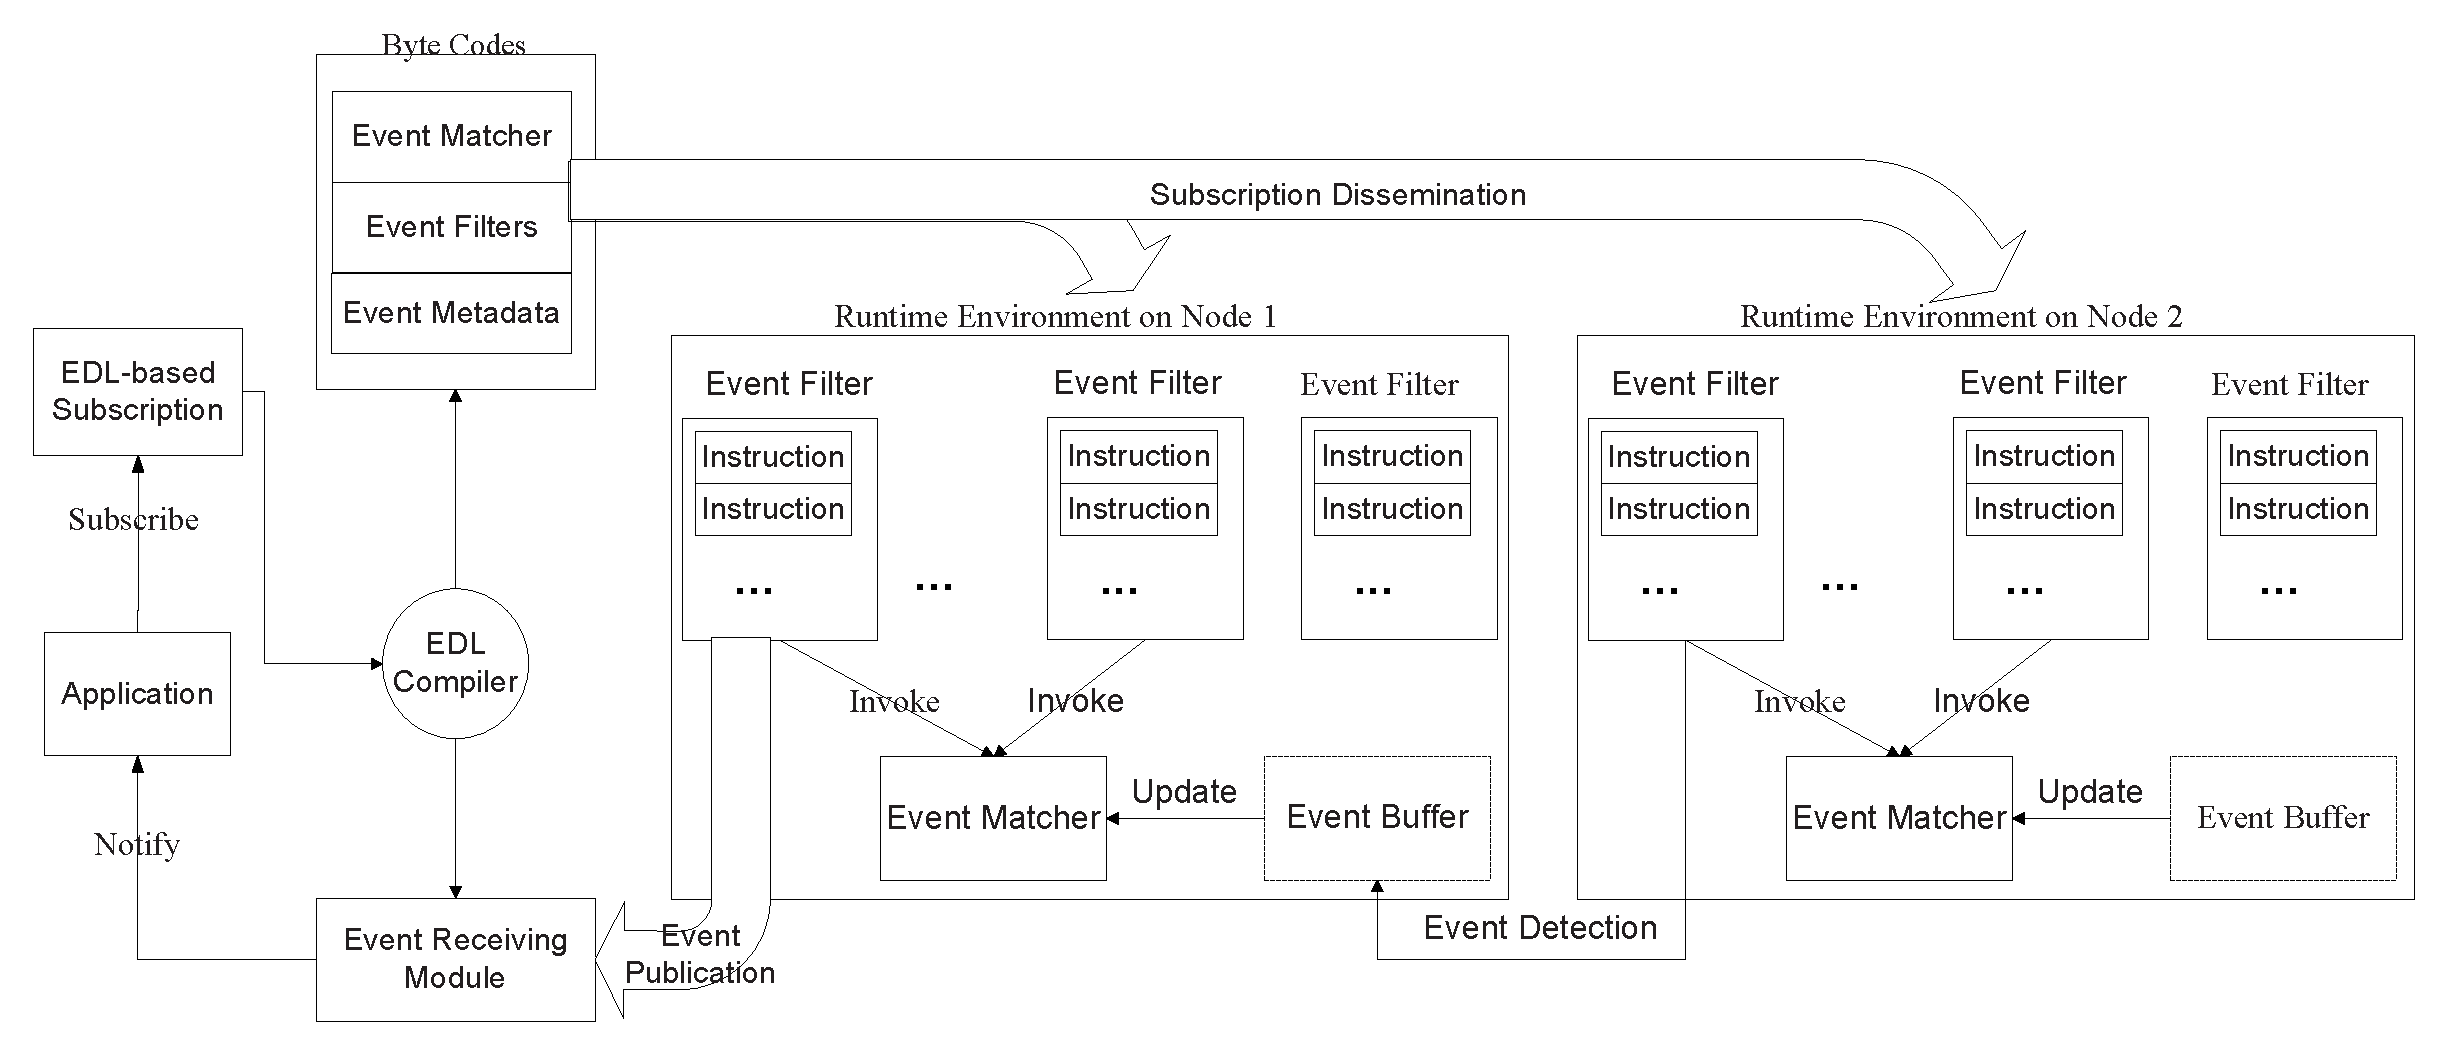
\includegraphics[width=\textwidth]{psware-interaction-simple}
\caption{PSWare components interaction}
\label{fig:psware-interaction-simple}
\end{figure*}
\subsection{Basic Instructions}
The design of our event detection framework makes it very suitable to be implemented using a VM-based architecture and this is how we implemented it in the bytecodes for the sensor nodes. Our VM-based runtime environment is based on Mat\'{e} \cite{mate}. It uses stack-based instructions which allow compact code size. We choose a VM-based runtime environment because it is more flexible in terms of interfacing with the EDL compiler and introducing new modules. Apart from the existing instructions which are already available in Mat\'{e}, we have mainly added the following instructions used specifically for event detection.
\begin{itemize}
	\item \emph{OPref}: whenever an event \(e\) is being evaluated, this instruction is invoked to obtain an instance of such event.
	\item \emph{OPoffset}: this instruction is involved right after the 'ref' instruction, in order to access individual attributes of the event instance.
	\item \emph{OPset}: if the attributes of an event need to be changed, this instruction will be used.
	\item \emph{OPget}: the 'get' instruction does the opposite of 'set' instruction. It will simply retrieve content of a specific attribute in an event.
	\item \emph{OPcreate}: is used to create a new instance of an event.
	\item \emph{OPeval}: is used to determine if an event happens or not.
\end{itemize}
For a complete list of all the instructions, please refer to Appendix \ref{appendix:isa} We give a simple example how EDL can be translated to the lower level runtime instruction sets. Consider a very simple event shown in Listing \ref{lst:originaledl}. The event will occur when the temperature reading on sensor node 5 is above 30. It's corresponding program for the VM is shown in Listing \ref{lst:translatededl}. Since 'SimpleEvent' is a primitive event, so every time it is being detected, a new instance of the event will be created. The ID of 'SimpleEvent' is \(1\). Here we also have another event called 'System' which is a built-in event provided by EDL as a place where all the sensor data can be obtained. The 'System' event has a default ID of \(0\) as shown on Line \ref{line:systemevent} in Listing \ref{lst:translatededl}. Each attributes in the event will have it's unique ID. In the example, the ID of the attribute is calculated simply by the order of their appearance. For example, temperature has the ID of \(0\) on Line \ref{line:systemevent}.

\begin{lstlisting}[caption=Original EDL program, label=lst:originaledl]
Event SimpleEvent {
	int temp=System.temp;
	int id=System.id;
} where {
	temp > 30 and
	id == 5
}
\end{lstlisting}
\begin{lstlisting}[caption=Translated EDL program, label=lst:translatededl]
alloc 1
ref 0 (*\label{line:systemevent}*)
offset 0
ref 1
offset 0
set
ref 0
offset 1
ref 1
offset 1 (*\label{line:idattr}*)
set
ref 1
offset 1
get
push 30
gt
ref 1
offset 1
get
push 5
eq
and
eval
\end{lstlisting}

\subsection{Customizing PSWare}
The event detection framework of PSWare is developed using NesC. As discussed in the previous section, many of the operations in PSWare can be defined according to applications. In this section, we describe how we can customize PSWare.

The first step is to implement a special module which acts like a device driver for PSWare. This module defines the sampling rate and a primitive event called 'System'. All the fields of other events are obtained from 'System'. The module needs to implement three interfaces: StdControl, SystemClock and SystemEvent as shown in Listing \ref{lst:systemEvent}. StdControl is a module for initialization purpose. SystemClock defines the sampling frequency. SystemEvent is used to obtain the pointer to the 'System' event.

\begin{lstlisting}[caption=API of the 'System' event, label=lst:systemEvent]
module SystemEventM {
	provides {
		interface StdControl;
		interface SystemEvent;
		interface SystemClock;
	}
}
interface SystemEvent {
	command EventInstanceInfo * get();
}
\end{lstlisting}

Once the 'System' event is defined, the application developers can further define their own functions for event delivery and event forwarding. We will show some examples in the next section. In addition, they can make use of the API provided by PSWare as shown in Listing \ref{lst:pswareAPI}.

\begin{lstlisting}[caption=API provided by PSWare, label=lst:pswareAPI]
interface EventMeta {
	command EventMetaInfo * getEventMeta(uint8_t subID);
	command bool isSubscribed(uint8_t subID);
	command bool isComposite(uint8_t subID);
	command bool isAggregate(uint8_t subID);
}
interface EventInstance {
	command EventInstanceInfo * createEvent(uint8_t subID);
	command int instanceAmount(uint8_t subID);
	command void deleteEvent(uint8_t subID, uint8_t instanceID);
	command EventInstanceInfo * getEventInstance(uint8_t subID, int idx);
}
interface EventMatcher {
	command bool selectSubevent(EventInstanceInfo * composite, EventInstanceInfo * subevent);
	command result_t eventDetected(uint8_t subID, uint8_t instanceID, bool detectionResult);
	command result_t eventDelivery(uint8_t subID, uint8_t instanceID, bool detectionResult);
}
\end{lstlisting}

These API provides the necessary functionalities for accessing modules such as event meta data or the event buffer (as in EventInstance). To implement application specific event detection mechanisms, application developers simply need to override the commands provided in the EventMatcher interface. The 'selectSubevent()' command is used to determine if a sub-event (in the parameter subevent) should be used to detect a composite event (in the parameter composite).
%\section{Complete List of the Instructions for EDF}
\label{appendix:isa}
In this section, we show the complete list of instructions currently used by our Event Detection Framework (EDF). We also briefly describe the function and the usage of each instruction.

\subsection{Basic Instructions}
The basic instruction deals with the most fundamental operations. Since the instruction uses a stack-based architecture in order to reduce the code size, most of the instructions that fall into this category deal with the operations related stacks.
\begin{itemize}
\item \emph{OPpush}: this instruction is used to push an operand to the top of the stack.
\item \emph{OPpop}: this instruction is used to pop and discard an operand from the top of the stack.
\item \emph{OPcopy}: duplicates the top operand of the stack
\item \emph{OPhalt}: once this instruction is reached, the VM will stop execution.
\end{itemize}

\subsection{Operators}
Basic mathematical operators:
\begin{itemize}
\item \emph{OPadd}: pops two operands off the top of the stack, add them together and push the result back to the top of the stack.
\item \emph{OPmult}: pops two operands off the top of the stack, multiply them together and push the result back to the top of the stack.
\item \emph{OPsub}: pops two operands off the top of the stack, subtract the first popped number by the second one and push the result back to the top of the stack.
\item \emph{OPdiv}: pops two operands off the top of the stack, divide the first popped number by the second one and push the result back to the top of the stack.
\item \emph{OPmod}: pops two operands off the top of the stack, divide the first popped number by the second one and push the remainder back to the top of the stack.
\item \emph{OPinv}: pops one operand (n) off the top of the stack, calculate its inverse (-n) and push the result back.
\end{itemize}

Logical operators:
\begin{itemize}
\item \emph{OPand}: pops two operands off the top of the stack, calculate the logical and of them and push the result back to the top of the stack.
\item \emph{OPor}: pops two operands off the top of the stack, calculate the logical or of them and push the result back to the top of the stack.
\item \emph{OPxor}: pops two operands off the top of the stack, calculate the exclusive or of them and push the result back to the top of the stack.
\item \emph{OPnot}: pops one operand off the top of the stack, calculate the logical not of it and push the result back to the top of the stack.
\end{itemize}

Relational operators:
\begin{itemize}
\item \emph{OPeq}: pops two operands off the top of the stack, if the two operands are equal, push 1 to stack. Otherwise, push 0 to stack.
\item \emph{OPneq}: pops two operands off the top of the stack, if the two operands are equal, push 0 to stack. Otherwise, push 1 to stack.
\item \emph{OPgt}: pops two operands off the top of the stack, if the first operand is greater than the second one, push 0 to stack. Otherwise, push 1 to stack.
\item \emph{OPgte}: pops two operands off the top of the stack, if the first operand is greater than or equal to the second one, push 0 to stack. Otherwise, push 1 to stack.
\item \emph{OPlt}: pops two operands off the top of the stack, if the first operand is less than the second one, push 0 to stack. Otherwise, push 1 to stack.
\item \emph{OPlte}: pops two operands off the top of the stack, if the first operand is less than or equal to the second one, push 0 to stack. Otherwise, push 1 to stack.
\end{itemize}

Bitwise operators:
\begin{itemize}
\item \emph{OPshiftl}: pops two operands off the top of the stack, left shift the first popped number by the second one and push the result back to the top of the stack.
\item \emph{OPshiftr}: pops two operands off the top of the stack, right shift the first popped number by the second one and push the result back to the top of the stack.
\item \emph{OPland}: pops two operands off the top of the stack, calculate the bitwise and of them and push the result back to the top of the stack.
\item \emph{OPlor}: pops two operands off the top of the stack, calculate the bitwise or of them and push the result back to the top of the stack.
\item \emph{OPxor}: pops two operands off the top of the stack, calculate the bitwise exclusive or of them and push the result back to the top of the stack.
\item \emph{OPlnot}: pops one operand off the top of the stack, calculate its complement and push the result back to the top of the stack.
\end{itemize}

\subsection{Event-related Instructions}
\begin{itemize}
\item \emph{OPref}: whenever an event \(e\) is being evaluated, this instruction is invoked to obtain an instance of such event.
\item \emph{OPoffset}: this instruction is involved right after the 'ref' instruction, in order to access individual attributes of the event instance.
\item \emph{OPset}: if the attributes of an event need to be changed, this instruction will be used.
\item \emph{OPget}: the 'get' instruction does the opposite of 'set' instruction. It will simply retrieve content of a specific attribute in an event.
\item \emph{OPcreate}: is used to create a new instance of an event.
\item \emph{OPeval}: is used to determine if an event happens or not.
\item \emph{OPgc}: used by the event matcher for garbage collection.
\end{itemize}
\section{PSWare: Model and Architecture}
\label{sec:model}
In this section, we describe the application programming model for PSWare. We keep the issues that described in Section \ref{sec:introduction} when establishing our model.

\subsection{Overview}
\begin{figure}
\centering
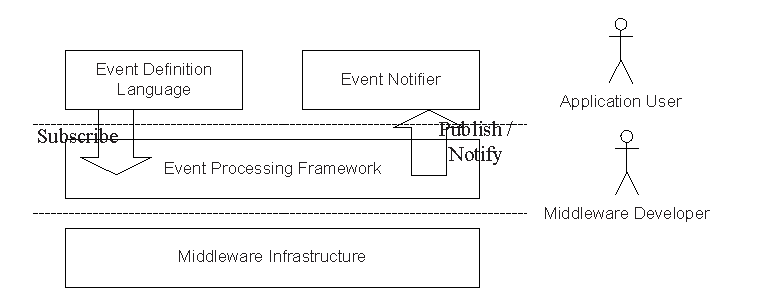
\includegraphics[width=\textwidth]{programmingModel}
\caption{PSWare programming model}
\label{fig:programmingModel}
\end{figure}

As shown in figure \ref{fig:programmingModel}, our model mainly has two different types of people that make use of two APIs of different levels:
\begin{itemize}
\item Application developers will make use of the event definition language to define and subscribe events and use the event receiving module to receive the published events.
\item Middleware developer will make use of the event processing framework to implement effective and efficient event processing algorithms
\end{itemize}

The first type is the application users. These users are responsible for defining and subscribing to high level events for different types of applications. They use a high level event definition language to translate the application requirements into events. They do not have to worry about the underlying event detection mechanisms.

On the lower level, we have another type of users called middleware developers. These users are responsible for implementing domain-specific event processing mechanisms. PSWare provides a couple of interfaces in TinyOS to make the implementation easier.

The benefit for such model is its flexibility. There are usually many different types of applications for a specific application domain. For example, in ITS, we may have collision warning, traffic flow control and overspeed detection yet these applications can probably share a lot of common event detection mechanisms. Therefore, the middleware developer only needs to implement the event processing mechanism for once. Then by defining different events, we can easily meet different application requirements without sacrificing the efficiency.

\subsection{Event Definition Language}
\begin{figure}
\centering
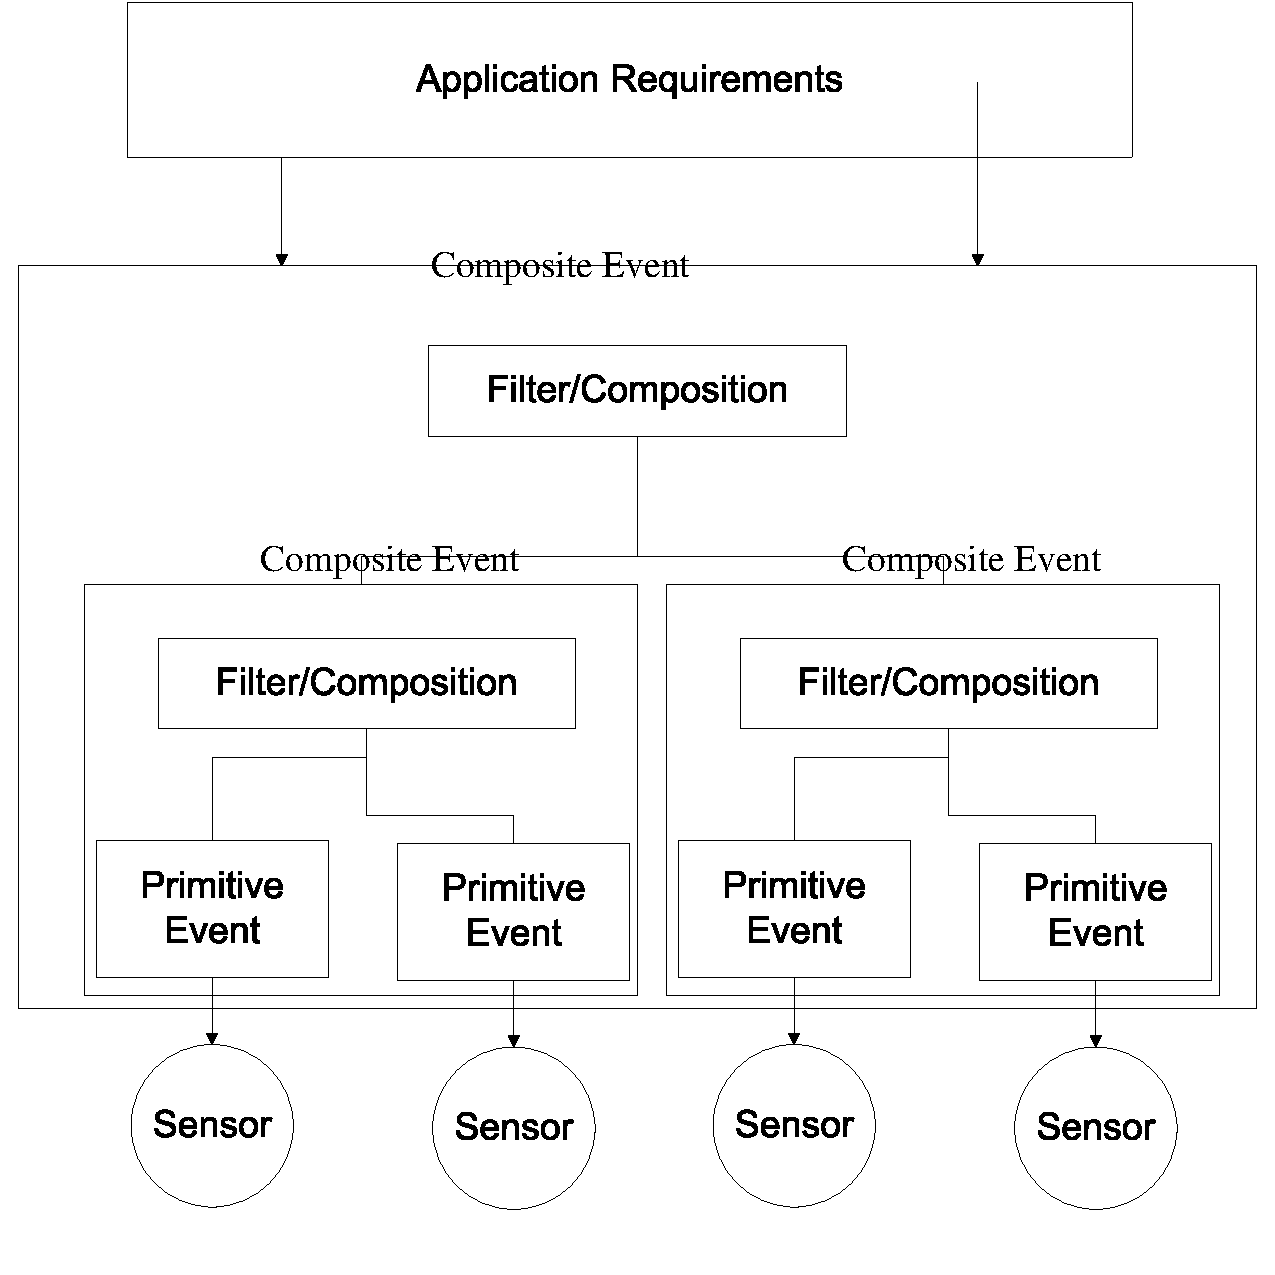
\includegraphics[width=.6\textwidth]{eventprogramming}
\caption{Type-based event model}
\label{fig:eventprogramming}
\end{figure}

PSWare will provide an type-based event programming model to the application user. Such model has the following characteristics:
\begin{itemize}
\item Each event type is similar to a class in object-based programming model. Similarly, event hierarchy in Figure \ref{fig:eventhierarchy} is similar to class hierarchy.
\item Similar to object-based model, attributes are encapsulated in each events.
\item Event definition are declarative. The high-level application developers only need to specify the event filters and event relations through operators and functions. The underlying mechanisms for implementing these operators are left to our event detection framework.
\end{itemize}

Figure \ref{fig:eventprogramming} conceptually shows our event model. On the top level, the application requirements are expressed in terms of the composite events that need to be detected. The composite events may be further divided into sub-events. Eventually all composite events can be divided into primitive events which can be directly detected by individual sensor nodes.

To re-use our example in Section \ref{sec:introduction}, Figure \ref{fig:rooms}, we may define the events as shown in Listing \ref{lst:rooms}.
\begin{lstlisting}[caption=Example of using even-based programming model, label=lst:rooms]
Event SimpleEvent {
	int temp=System.temp;
	int id=System.id;
	int time=System.time;
} where {
	temp > 30
}
Event CompEvent {
} on {
	SimpleEvent e1 and
	SimpleEvent e2
} where {
	e1.Location="A" and
	e2.Location="B" and
	e2.time-e1.time=600
}
\end{lstlisting}

We can see that our event-based programming model shares some of the similarity with SQL, especially for the event filters, which consist of operators. In this particular example, we have two event types. On the top level, the application wants to monitor the temperature change so the event type 'CompEvent' is defined. 'CompEvent' consists of two sub-events of the same type: SimpleEvent. Note that our programming model is declarative. The user just specifies the event types and the corresponding filters without specifying the event detection strategies described in Section \ref{sec:introduction} because that part is left to the event detection framework. We will go into more details in that in the latter part of this section.

\subsection{Event Notifier}
Apart from submitting event definition, the application user needs to be notified when the subscribed events are detected by WSN. This is done through event notifier. When the application user subscribes events, the user needs to pass an additional object as the event notifier. When the subscribed event is detected, PSWare will notify the user with this notifier object. Listing \ref{lst:notiferJava} shows our notifier class implemented and how it is related to the subscription class.

\begin{lstlisting}[caption=Event notifier in Java, label=lst:notiferJava]
public interface EventNotifier {
	public void notify(String eventStr);
	...
}
public class EventSubscription {
	public Boolean subscribe(String subscription, EventNotifier notifier) {
		...
	}
}
\end{lstlisting}

While Listing \ref{lst:notiferJava} shows the notifier in Java, bindings for other languages can be created in similar fashion. A Python binding is shown in Listing \ref{lst:notiferPython}.
\begin{lstlisting}[caption=Python binding of event notifier, label=lst:notiferPython]
class EventNotifier:
	def notify(self, eventStr):
		pass
class EventSubscription:
	def subscribe(self, subscription, notifier):
		...
\end{lstlisting}

Upon the detection of events, the notifier will be invoked so that the events can be delivered to the user. The event is delivered as a string, with each attribute assigned with an actual value. As an example, suppose the user has subscribed to the event 'SimpleEvent' in Listing \ref{lst:rooms}, then when the event is detected by PSWare, it will be delivered to the user with the content shown in Listing \ref{lst:eventFormat}.
\begin{lstlisting}[caption=Received event from notifier, label=lst:eventFormat]
SimpleEvent e1 {
	temp=32;
	id=0;
	time=13345;
}
\end{lstlisting}

\subsection{API for Event Processing Framework}
The event processing framework of PSWare is developed using NesC. PSWare also provides a group of APIs for the middleware developers to write customized event processing algorithms. First, since all events can ultimately be decomposed into primitive events, the middleware developer needs to first define the required primitive events used in the application domain. This is done through a configuration named 'PrimitiveEventC'. It is listed in Listing \ref{lst:primitiveEvent}. The new event ID should be defined as an enumeration in PSWare's header file.
\begin{lstlisting}[caption=Primitive event component in NesC, label=lst:primitiveEvent]
generic configuration PrimitiveEventC(evet_id_t eventId) {
  provides {
    interface Read<uint16_t>;
  }
} implementation {
	...
}
\end{lstlisting}

In PSWare, everything is treated as events and that includes temperature, photo and even timer. Similar to other generic components in TinyOS, if necessary, new events can be added by implementing a new event ID. Once set, we need to create a higher level primitive event so that the application users can make new event definitions based on top of it. This is done by an automatic tool which will be invoked when building and output a class which will be used by the event notifier and an event definition which will be used by EDL.

When this is set, the application user can already start to subscribe and detect events by using PSWare's default event detection algorithm: TED \cite{lai:ted}. If the middleware developer wants to write their own event detection algorithm, they can choose to implement two interface 'EventMatcher' and 'EventDeliver' as shown in Listing \ref{lst:pswareEventMatcher}. The 'EventMatcher' interface includes two major event which serves three purposes as follows:
\begin{enumerate}
\item During the execution of the middleware, the network may detect multiple events for a single event type. Therefore, upon the detection of the composite events, the event detection algorithm may choose a specific event from one of this sub-types for detection. This is done by signaling the first event 'select sub-event'.
\item Upon the detection of an event, the event detection algorithm may perform some customized processing to update some information so that the next time when the event happens again, it may be detected with lower cost. This is when the second event 'eventMatched' comes into play. The middleware developer may implement customized event processing mechanisms according to the matched events.
\end{enumerate}

Apart from event matcher, we also have an event deliverer which will be called when a subscribed event is detected. The middleware developer may implement its only function to meet the requirements for event delivery. This is done when the middleware signals the 'eventDeliver' event.
\begin{lstlisting}[caption=The event matcher interface, label=lst:pswareEventMatcher]
interface EventMatcher {
	event bool selectSubevent(EventInstanceInfo * composite, EventInstanceInfo * subevent);
	event result_t eventMatched(evet_id_t eventId, evet_id_t instanceID, bool detectionResult);
}
interface EventDeliverer {
	event result_t eventDeliver(evet_id_t eventId, evet_id_t instanceID, bool detectionResult);
}
\end{lstlisting}

To facilitate the implementation of event matcher and event deliverer, the middleware developer can make use of the APIs provided by PSWare in Listing \ref{lst:pswareAPI}. These APIs are mostly used to retrieve the event information.
\begin{lstlisting}[caption=PSWare API in NesC, label=lst:pswareAPI]
interface EventType {
	command EventTypeInfo * getEventType(evet_id_t eventId);
	command bool isSubscribed(evet_id_t eventId);
	command bool isComposite(evet_id_t eventId);
}
interface EventInstance {
	command int instanceAmount(evet_id_t eventId);
	command EventInstanceInfo * getEventInstance(evet_id_t eventId, evet_id_t idx);
	command void deleteEvent(evet_id_t eventId, evet_id_t instanceID);
}

typedef struct {
	evet_id_t eventId;
	evet_id_t level;
	size_t size;
} EventTypeInfo;

typedef struct {
	evet_id_t typeID; (*\label{lst:pswareAPI:typeID}*)
	evet_id_t instanceID;
	uint16_t * attributes;
} EventInstanceInfo;
\end{lstlisting}

The first interface, 'EventType' has three commands. The first command is for the individual event instances to obtain the type information based on their type ID as shown on line \ref{lst:pswareAPI:typeID}. The second and the last commands are self-explanatory. They are used to determine if a given event type is a composite event or is subscribed by the user.

Since for each event type, there can be multiple events, we need the second interface 'EventInstance' to process those events. There are three commands for this interface. The first one is used to obtain the number of the events for a specific type currently stored in the event buffer on the sensor node. We will discuss about the event buffer in the next section. Upon knowing the number of events, the middleware developer can iterate through the event list and use the second command to get the events. As for the last command, when an event is detected to be useless, the middleware developer may delete it from the list.

The data structures are shown after the interfaces. For event type, we have the ID for the type, its level in the subscribed event tree and its size. For the event instance data structure, we have its type ID, instance ID and its attribute list. If the event contains some attributes of the primitive events, they can be obtained here by using the index defined in the enumeration value for primitive event. For instance, if one of the primitive event has an enumeration value labeled 'EVENT\_LIGHT', then if the event instance also has one of its attribute from the sensor's light reading, the middleware developer can access it by writing 'attributes[EVENT\_LIGHT]'.

In summary, the middleware developer may follow the following steps to implement customized event detection algorithms:
\begin{itemize} 
\item Implement new primitive event types if necessary.
\item Define the event matcher for how sub-events are selected for matching and what to do after a predefined event type is detected.
\item Define customized function for event delivery.
\end{itemize}
\begin{figure}
\centering
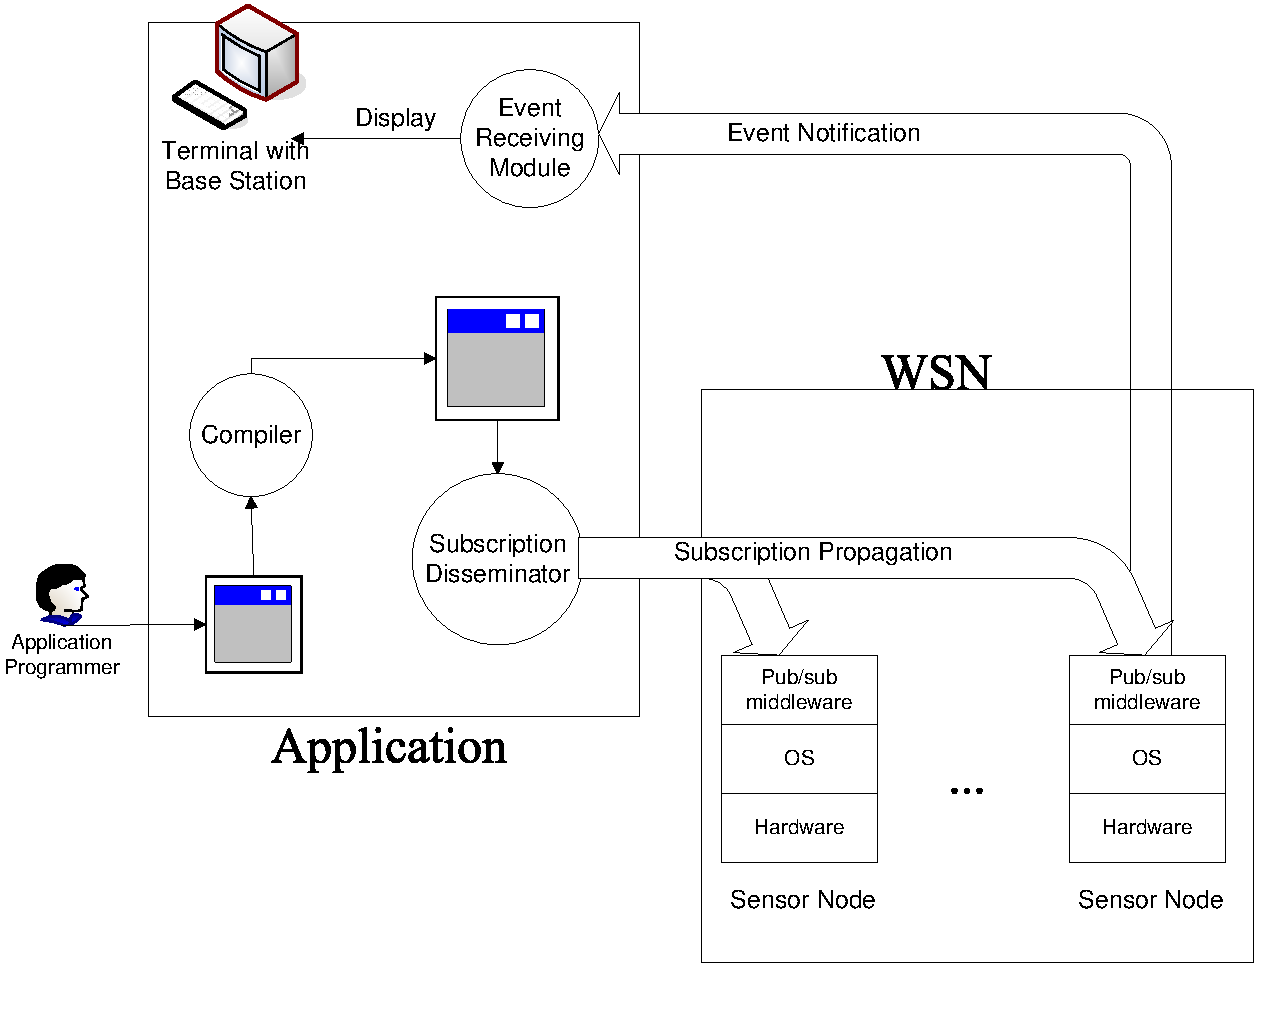
\includegraphics[width=.6\textwidth]{psware-architecture}
\caption{Event processing in PSWare}
\label{fig:psware-architecture}
\end{figure}

\section{Composite Event Processing in PSWare}
\label{sec:design}
In this section, we discuss how PSWare is designed to support composite event. The overall work flow of event processing in PSWare is shown in Figure \ref{fig:psware-architecture}. To use the middleware, applications developers will first define event types according to the application requirements. The subscription will then be compiled and processed by the EDL compiler and be disseminated into the network. When the events are detected by sensor nodes, they will be delivered to the application.

\subsection{Event Specification}
\begin{figure}
\centering
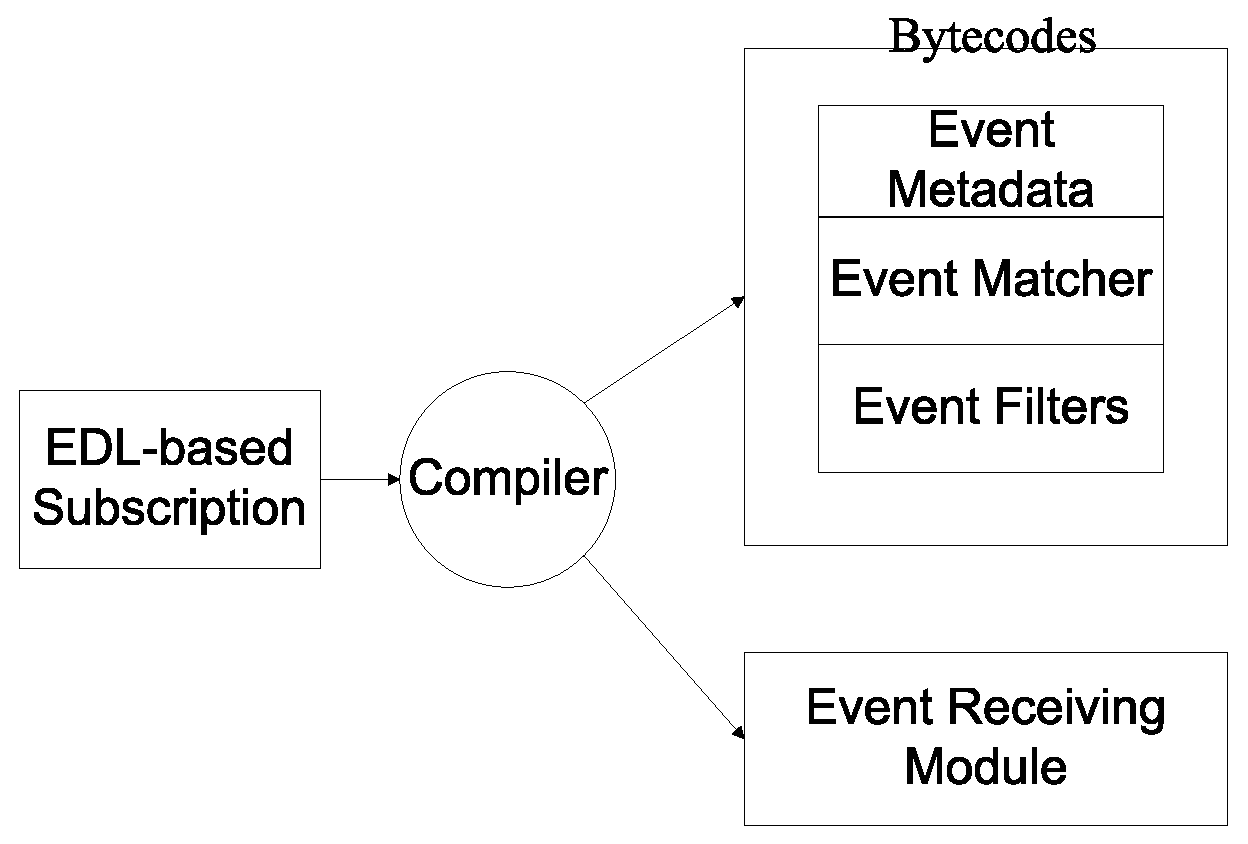
\includegraphics[width=.7\textwidth]{edlcompiler}
\caption{PSWare-EDL compiler structure}
\label{fig:edlcompiler}
\end{figure}

EDL is used for specifying events in PSWare. For each EDL script, it contains one or more event definition and one subscribing statement. Formally, the Backus-Naur Form (BNF) of the subscription is defined in Listing \ref{lst:BNFSubscription}.

\begin{lstlisting}[caption=BNF (simplified) of subscription, label=lst:BNFSubscription]
subscription -> event_declarations subscribe_statement
event_declarations -> event_declaration | event_declarations event_declaration
subscribe_statement -> SUBSCRIBE IDENTIFIER SEMICOLON
\end{lstlisting}

The subscribe statement simply uses the keyword 'subscribe' followed the event type name needed by the application. Each event type declaration can have up to three parts: the event body, the \emph{where} clause and the \emph{on} clause. The event body defines the attributes of the events. The \emph{on} clause are used to specify the sub-events used by a composite event. The \emph{where} clause defines the filter of the corresponding event type. Formally, the BNF of event type is defined in Listing \ref{lst:BNFEvent}

\begin{lstlisting}[caption=BNF (simplified) of event type, label=lst:BNFEvent]
event_declaration -> EVENT IDENTIFIER event_body on_clause_opt where_clause_opt
event_body -> { field_declarations_opt }
on_clause -> ON { subevent_declarations_opt }
where_clause -> WHERE { conditional_expression }
\end{lstlisting}

The \emph{on} clause and the \emph{where} clause are both optional in case the event is primitive or does not have a filter. The on clause looks similar to the field declaration except sub-events instead of fields are declared. This is done for a clear code presentation and easier type checking. The where clause simply consists of conditional expressions so that the filters may be defined by specifying the operators.

\begin{comment}
A simple example of using EDL is shown in Listing \ref{lst:originaledl}. In this example, two events, 'SimpleEvent' and 'CompEvent' are defined. 'SimpleEvent' is a primitive event which occurs when the detected temperature reading is above certain threshold. 'CompEvent' is a composite event that is based on two events of 'SimpleEvent' and their time must satisfy a certain condition in order to indicate the occurrence of 'CompEvent'.
\begin{lstlisting}[caption=A simple EDL program, label=lst:originaledl]
Event SimpleEvent {
	int temp=System.temp;
	int id=System.id;
	int time=System.time;
} where {
	temp > 30
}
Event CompEvent {
} on {
	SimpleEvent e1 and
	SimpleEvent e2
} where {
	e2.time-e1.time=600
}
\end{lstlisting}
\end{comment}

The EDL-based subscription will be processed by our EDL compiler. The output of the compiler has two parts as shown in Figure \ref{fig:edlcompiler}. The first part is the byte codes which will be executed by individual sensors to detect events. The format and the organization of the byte codes are closely related to the event processing framework and customization of PSWare. We will go through these topics in the following sections.

\begin{figure}
\centering
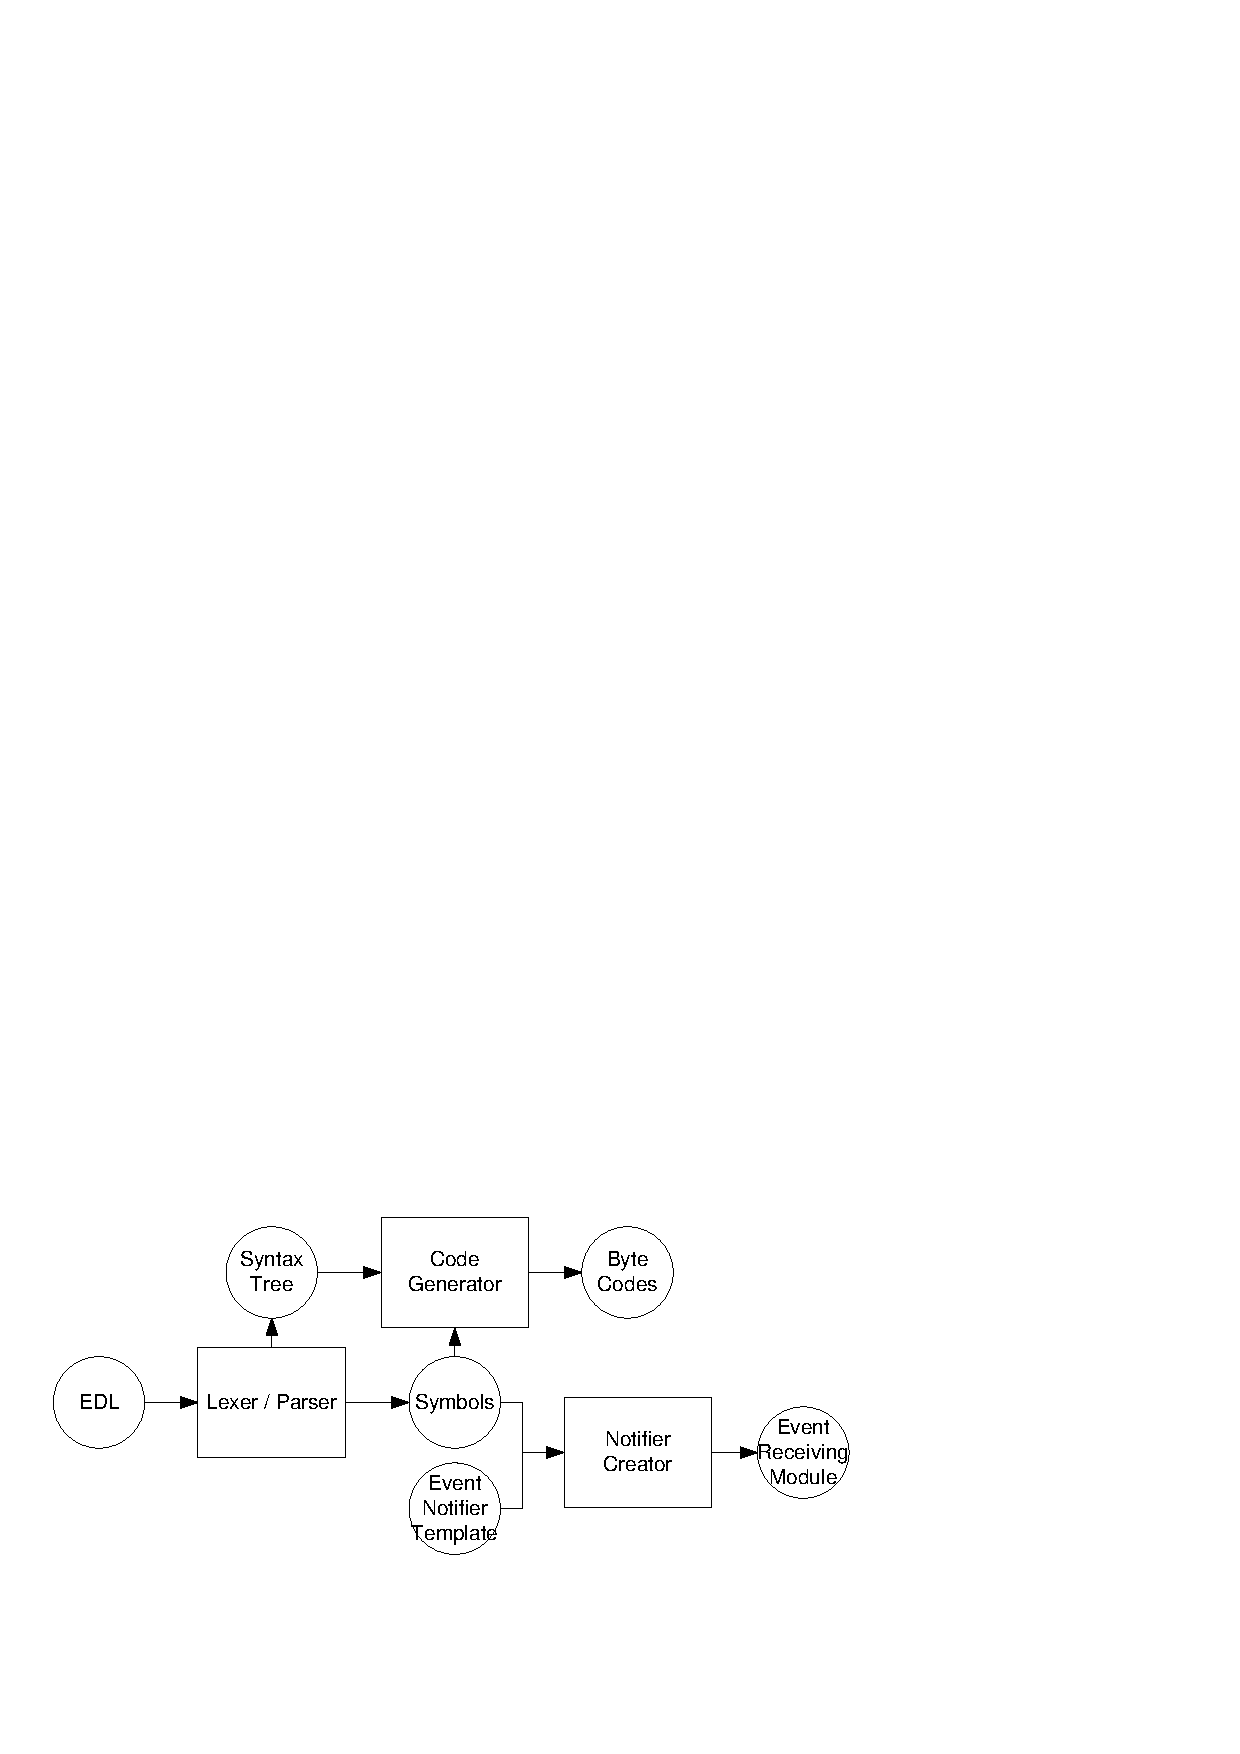
\includegraphics[width=.8\textwidth]{edlcompiler-flow}
\caption{EDL compiler flow}
\label{fig:edlcompiler-flow}
\end{figure}

The second part, the event receiving module is the implementation of the event notifier as discussed in Section \ref{sec:model}. As shown in Figure \ref{fig:edlcompiler-flow}, The EDL compiler will execute the following steps in order to generate the byte codes and event receiving module:
\begin{enumerate}
\item Parse the EDL script and generate the corresponding syntax tree and symbol table.
\item Generate the byte codes based on the syntax tree and symbol table.
\item Create the event receiving module based on the symbol table.
\end{enumerate}

\subsection{Runtime Environment for Event Detection}
The byte codes generated by the compiler can be further divided into three parts: event meta data, event filters and event matcher. These components implements the programming interface discussed in Listing \ref{lst:pswareEventMatcher} and \ref{lst:pswareAPI}. Event meta data contains the description of the event types such as event type ID, event size and the individual attributes for each event. Event filters are the constraints defined for each event type. Event matcher schedules the execution for event detection according to the subscription and event relations.

The runtime environment on each sensor node is similar to the VM-based approach \cite{mate} in the sense that subscriptions are broken down into some basic operations called instructions. For a complete list of instructions, please refer to the Appendix. Such design choice is for extensibility so that new features can be added more easily by adding new instructions. In addition to the VM-based runtime environment, each sensor node has an event buffer where the detected events can be stored for composite event detection.

\begin{figure}
\centering
\figurecurrentwidth{eventdetectionframework2}
\caption{PSWare runtime environment}
\label{fig:eventdetectionframework2}
\end{figure}
The essential operations for our runtime environment are shown in Figure \ref{fig:eventdetectionframework2}. In this environment, the event matcher will first fetch the events from the event buffer and then evaluate them against the corresponding filters. If the event has been detected, then it will be transmitted over the network. Formally, the procedure of the event matcher can be shown in Procedure \ref{algo:eventmatcher} with some notations defined as:
\begin{itemize}
\item Event types: \(E=\{e_1, e_2 \cdots \}\)
\item For each \(e_n\in E\), its filter is: \(e_n\rightarrow filter\)
\item For each \(e_n\in E\), it has a set of events \(E_n=\{e_n^1, e_n^2 \cdots \}\) stored in the buffer.
\end{itemize}

\begin{algorithm}
\begin{algorithmic}
\REQUIRE \(E\)
	\FORALL {\(e_n\in E\)}
		\FORALL {\(e_n^i\in E_n\)}
			\IF {\(e_n\) is primitive}
				\STATE result = evaluate\_primitive (\(e_n^i\))
				\IF {result == True}
					\STATE eventMatched(\(e_n^i\))
					\IF {\(e_n\) is subscribed}
						\STATE deliver(\(e_n^i\))
					\ELSE
						\STATE forward(\(e_n^i\))
					\ENDIF
				\ENDIF
			\ELSE
				\STATE \(e_{sub} = \emptyset \)
				\FORALL {subevents \(e_m\) for \(e_n\)}
					\STATE \(e_{sub} = e_{sub}\bigcup selectSubevent (e_n, e_m)\)
				\ENDFOR
				\FORALL {subevents \(e_m\) for \(e_{sub}\)}
					\STATE evaluate\_composite(\(e_n^i\), \(e_m\), \(\cdots \))
				\ENDFOR
			\ENDIF
		\ENDFOR
	\ENDFOR
\end{algorithmic}
\caption{Procedure of the event matcher}
\label{algo:eventmatcher}
\end{algorithm}

There are several keys in the procedure. First, when the event matcher picks up the events of type \(e_n\) from the event buffer, it may use application specific mechanisms to pick up the desired events instead of trying all the possible combinations. Second, the 'deliver()' and the 'forward()' function are used to deliver the subscribed events or forward the events so that composite events may be detected. These two functions may also be application dependent to achieve high energy efficiency.

\begin{comment}
Figure \ref{fig:psware-interaction-simple} illustrates how different components in the middleware system interact with each other.

\begin{figure}
\centering
\figurecurrentwidth{psware-interaction-simple}
\caption{PSWare-E components interaction}
\label{fig:psware-interaction-simple}
\end{figure}
\subsection{PSWare Customization}
\end{comment}

Finally, it is necessary to mention the 'SystemEvent'. This module acts as the device driver for PSWare. It defines the sampling rate and a primitive event. All the fields of other events are obtained from 'System'. The module needs to implement three interfaces: StdControl, SystemClock and SystemEvent as shown in Listing \ref{lst:systemEvent}. StdControl is a module for initialization purpose. SystemClock defines the sampling frequency. SystemEvent is used to obtain the pointer to the 'System' event.

\begin{lstlisting}[caption=API of the 'System' event, label=lst:systemEvent]
module SystemEventM {
	provides {
		interface StdControl;
		interface SystemEvent;
		interface SystemClock;
	}
}
interface SystemEvent {
	command EventInstanceInfo * get();
}
\end{lstlisting}

The 'SystemEvent' is there so that needs to be implemented by the middleware developers as the  Once the 'System' event is defined, the application developers can further define their own functions for event delivery and event forwarding. We will show some examples in the next section. 
\section{Support for Customization in PSWare}
\label{sec:flexibility}
An important feature of PSWare is that it can be customized. To support customization, PSWare uses a flexible layered architecture. In this way, developers can customize different layers without affecting each other. Moreover, multiple event processing strategies may be dynamically used during the runtime. In this section, we how such customization can be done at different layers. These layers consist different aspects of a complete event-based system, including, event detection, event delivery and event subscription.

\subsection{Customizable Event Definition}
It is a common scenario for the applications to define extra event attributes that have domain-specific meanings. For example, in an application which requires reliable communication, we might want to define a probability value which specifies the threshold for the message loss. Then in the middleware framework, this number should be used during the actual communication.

The simplest way to pass some domain-specific information to the middleware is to modify the System event. As discussed in Section \ref{sec:design}, the System event is used like a device driver that represents the primitive events collected by the system. Internally, this event is specified in a header file and can be modified to suit different applications. The essential steps are as follows:
\begin{enumerate}
\item Modify 'SystemEvent.h' and add necessary attributes for the system event
\item Use 'psware gen' to generate the necessary constant values for accessing the new attribute in the middleware runtime environment
\item Modify the middleware framework so that the attributes can be used
\item Use the new attributes in the actual event definition
\end{enumerate}

We will illustrate these steps through an application scenario. Suppose the middleware developer has implemented a message retransmission mechanism for the event delivery and matching functions to make the application more reliable. Then the application developers can specify a parameter indicating the desired reliability for the events they define. The new 'SystemEvent.h' will look like in Listing \ref{lst:SystemEventProbability}.

\begin{lstlisting}[caption=Customized system event, label=lst:SystemEventProbability]
typedef struct {
	uint16_t nodeID;
	uint16_t time;
	float probability;
} SystemEvent;
\end{lstlisting}

Once the new probability attribute is defined, we need to generate some necessary constant values for accessing the attribute. The tool for generating the constants is 'psware gen'. It will parse the event header files and output some macro values. After that, the middleware can access the attribute with the code fragment shown in Listing \ref{lst:SystemEventProbabilityAccess}. In this piece of code, we first obtain the system event through the EventInstance API. Then we obtain the probability value by accessing the correct attribute. Note that SystemEvent, SystemEvent\_probability are generated constant values for accessing the events and their attributes.

\begin{lstlisting}[caption=Customized system event, label=lst:SystemEventProbabilityAccess]
EventInstanceInfo * systemPtr = call EventInstance.getEventInstance(SystemEvent);
float probability = (float)systemPtr->content[SystemEvent_probability];
\end{lstlisting}

The event probability can then be further defined through event definition. To reuse the event definition in Listing \ref{lst:rooms}, now if the user wants to add a parameter to indicate the reliability, he may insert a statement at Line \ref{lst:reliability:def} which defines the global reliability parameter.

\begin{lstlisting}[caption=Example of event definition with reliability, label=lst:reliability]
Event SimpleEvent {
	int temp=System.temp;
	int id=System.id;
	int time=System.time;
	System.reliability = 1.0; (* \label{lst:reliability:def} *)
} where {
	temp > 30
}
Event CompEvent {
} on {
	SimpleEvent e1 and
	SimpleEvent e2
} where {
	e1.Location="A" and
	e2.Location="B" and
	e2.time-e1.time=600
}
\end{lstlisting}

Once the parameter is defined. The information will be passed to the middleware and the corresponding code fragment in Listing \ref{lst:SystemEventProbabilityAccess} will work as expected.

\subsection{Customizable Event Detection}
Event detection is the heart of an event-based system. In PSWare, we can easily customize event detection on the event detection layer. Since PSWare uses a type-based event model to support composite event, event detection can also be customized according to the event types. The customization takes the following steps:
\begin{enumerate}
\item Define some domain-specific event types that requires specific event detection methods
\item Generate the necessary constant values for accessing the new attribute in the middleware runtime environment
\item Implement the specific event detection methods in the middleware
\end{enumerate}

We demonstrate the steps through a simple example, iTED. iTED is a simplified version of the TED \cite{lai:ted} algorithm, the default event detection algorithm in PSWare. We will discuss our default event detection algorithm, TED, in the chapter. Different from TED, iTED is customized for indoor monitoring application where the events are first fused in each monitored room. Then the results are further fused for global event detection. For simplicity, we assume each sensor node is equipped with a room ID and there maybe more than one fusion points in each room. However, all fusion points are selected in advance and will remain unchanged. The room ID can either be pre-deployed in the sensor nodes' program or be obtained using localization methods and more sophisticated fusion point selection methods may be implemented by extending some components discussed here.

\begin{figure}
\centering
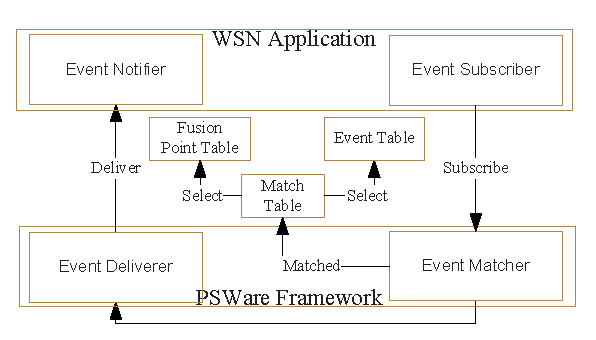
\includegraphics[width=.8\textwidth]{ted-architecture}
\caption{iTED over PSWare}
\label{fig:ted-architecture}
\end{figure}

Figure \ref{fig:ted-architecture} shows an overall diagram on how iTED interacts with PSWare. To implement iTED in PSWare, we need three key components:
\begin{enumerate}
\item Fusion point table: each sensor node updates this table in order to find the fusion point.
\item Event table: each sensor node maintains this table in order to decide if a given detected event should be forwarded to the fusion point.
\item Event matcher: a component that implements the event matching interface as discussed in Section \ref{sec:model}, Listing \ref{lst:pswareEventMatcher}.
\end{enumerate}

The first step is to add a new attribute, roomID, to our system event. This has already been discussed in the previous sub-section in Listing \ref{lst:SystemEventProbability} and we will skip it here. The only difference is the new attribute here will be of 'int' type instead of 'float' type.

Our first component, the fusion point table maintained by each sensor node \(v'_n\in V'\) is denoted as \(table_r\). It contains the following data:
\begin{itemize}
\item	Hop count (\(hop_n\)): the number of hops to reach the fusion point
\item	Parent (\(parent_n\)): the next hop to that fusion point
\end{itemize}

The procedure for updating fusion point table is shown in Procedure \ref{algo:ited:table_r}. Note that we make use of the roomID to filter the messages.
\begin{algorithm}
\begin{algorithmic}
\REQUIRE \(v_n\rightarrow msg_r\)
	\FOR {each entry \(t'\) in \(msg_r\)}
		\IF {\NOT exists \(t'\rightarrow fid_n\) in \(table_r\)}
			\STATE \(addTo(table_r, t')\)
		\ENDIF
		\FOR {each entry \(t\) in \(table_r\)}
			\IF {\(t\rightarrow roomID = t'\rightarrow roomID\)}
				\IF {\(t'\rightarrow hop_n < t\rightarrow hop_n\)}
					\STATE \(t\rightarrow hop_n \gets t\rightarrow hop_n+1\)
					\STATE \(t\rightarrow parent_n \gets v_n\)
				\ENDIF
			\ENDIF
		\ENDFOR
	\ENDFOR
	\IF {self is fusion point \AND \NOT exists \(self\rightarrow id\) in \(table_r\)}
		\STATE \(addTo(table_r, (self\rightarrow id, 0, self\rightarrow id))\)
	\ENDIF
	\STATE \(msg_r \gets table_r\)
	\STATE \(periodically\_broadcast(msg_r)\)
\end{algorithmic}
\caption{Fusion point table exchange}
\label{algo:ited:table_r}
\end{algorithm}

The second and the last component, the event table and the event matcher are closely related. Each sensor node will maintain an event table which is denoted as \(table_e\). The event table contains information for each event type \(e_n\in E\) as follows:
\begin{itemize}
\item Event type ID (\(e_n\)): the ID which is assigned to each event type
\item Fusion point for the event (\(fusion_n\)): the fusion point at which the event is mostly likely to be detected at the lowest cost.
\item Fusion cost (\(cost_n\)): the fusion cost for event type \(e_n\)
\end{itemize}

In addition, each fusion point \(v'\in V'\) will maintain another table, the event matching \(table_m\) for the purpose of matching events. \(table_m\) contains the following fields:
\begin{itemize}
\item Event type ID (\(e_n\)): the ID of the event type
\item Event instance ID (\(i\)): the \(i\)th event instance of event type \(e_n\) (we use \(e_n^i\) to denote such an instance of event)
\item Source node (\(v_n^i\)): the node which forwarded \(e_n^i\) to the fusion point
\item Event timestamp (\(t_n^i\)): the timestamp when the event \(e_n^i\) is detected
\item Detection cost (\(cost_n^i\)): the cost for detecting event \(e_n^i\)
\end{itemize}

First, each node \(v_n\) periodically broadcasts messages \(msg_r\) which is its \(table_r\). If the node itself is a fusion point, then it will add itself in \(table_r\) and broadcast the message. The procedure is shown in Procedure \ref{algo:ited:table_r}. In addition to \(msg_r\), each \(v'_k\in V'\) will periodically advertise its \(table_m\) by broadcasting \(msg_m\) so that other sensor nodes can construct their \(table_e\) with Procedure \ref{algo:ited:table_e}.

\begin{algorithm}
\begin{algorithmic}
\REQUIRE \(v'_k\rightarrow msg_m\)
	\FOR {each entry \(t'\) in \(msg_m\)}
		\IF {\NOT exists \(t'\rightarrow e_n\) in \(table_e\)}
			\STATE \(addTo(table_e, (t'\rightarrow e_n, 1, v'_k, t'\rightarrow cost_n^i+table_r\rightarrow hop_k))\)
		\ENDIF
		\FOR {each entry \(t\) in \(table_e\)}
			\IF {\(t\rightarrow e_n = t'\rightarrow e_n\)}
				\IF {\(t'\rightarrow cost_n^i+table_r\rightarrow hop_k < t\rightarrow cost_n\)}
					\STATE \(t\rightarrow cost_n \gets t'\rightarrow cost_n^i+table_r\rightarrow hop_k\)
					\STATE \(t\rightarrow fusion_n \gets v'_k\)
				\ENDIF
			\ENDIF
		\ENDFOR
	\ENDFOR
	\IF {self is fusion point}
		\STATE \(msg_m \gets table_m\)
		\STATE \(periodically\_broadcast(msg_m)\)
	\ENDIF
\end{algorithmic}
\caption{Event table exchange}
\label{algo:ited:table_e}
\end{algorithm}

The construction of \(table_m\) will take place when the event instance \(e_n^i\) is detected and forwarded to a fusion point \(v'_n\). We will discuss how forwarding could be done in the next subsection.

When an event \(e_n^i\) is matched at node \(v_k\), node will use \(table_r\) and \(table_e\) to decide how to forward the detected event to the fusion points so that higher level events can be matched. In case the fusion point for event type \(e_n\) has not been decided, the node will forward the event to some of its closet fusion points  according to iTED. Upon the reception of \(e_n^i\) from \(v_k\), the fusion point will first update its own \(table_m\). Then it will check if there is any composite event \(e_{comp}\) which uses \(e_n\) and another event \(e_j\) as its sub-event (\(e_{comp}=comp(e_n, e_j)\)). If there is, then \(e_j\) will be used upon 'selectSubevent'.

\begin{algorithm}
\begin{algorithmic}
\REQUIRE \(e_n^i\) matched by \(v_k\) with cost: \(cost_n^i\)
	\STATE \(addTo(table_m, (e_n, e_n^i, v_k, now(), cost_n^i))\)
	\FOR {each \(e_j\) in \(E\)}
		\IF {\(\exists r\in R\) \AND \(r=e_{comp}=comp(e_n, e_j)\)}
			\FOR {each \(e_j^k\) in \(table_m\)}
				\IF {\(comp(e_n^i, e_j^k)=true\)}
					\STATE \(addTo(table_m, (e_{comp}, e_{comp}^i, self, now(), cost_n^i+cost_j^k))\)
					\STATE \(detected(e_{comp})\)
				\ENDIF
			\ENDFOR
		\ENDIF
	\ENDFOR
\end{algorithmic}
\caption{Event matching}
\label{algo:ited:eventmatching}
\end{algorithm}

If \(e_{comp}\) has been successfully detected by the underlying event matcher, then Procedure \ref{algo:ited:eventmatching} will be executed so that \(table_m\) is updated accordingly and iTED may reduce the energy cost for future event detection. Note that Procedure \ref{algo:ited:eventmatching} will make use of the APIs in Listing \ref{lst:pswareAPI} since it needs to query the event relations.

\subsection{Customizable Event Delivery}
After the subscribed event is detected, it needs to be delivered to the user. In many applications, this is done via the underlying routing protocols such as CTP provided by TinyOS. This is also the case for the default event delivery in PSWare. However, in some applications, this may not be a case. For example, in an intelligent transportation system, the events may be delivered to mobile vehicles. In this subsection, we show how PSWare can achieve the flexibility in event delivery through several examples in ITS.

We choose ITS as an example because different event types in this application may require different event delivery strategies and that is why the flexibility in event delivery is of particular importance. The event types in ITS may include:
\begin{itemize}
\item Emergency: events that represent urgent incidents. Examples of this type of events include car accidents and urgent road maintenance. These events probably need to be delivered to all nearby vehicles when occurred.
\item Driver's information: events that provide assistant information to the drivers. Examples include congestion information and whether information These events are usually not considered as urgent and may be delivered in carry-and-forward fashion \cite{cartel}.
\end{itemize}

\begin{figure}
\centering
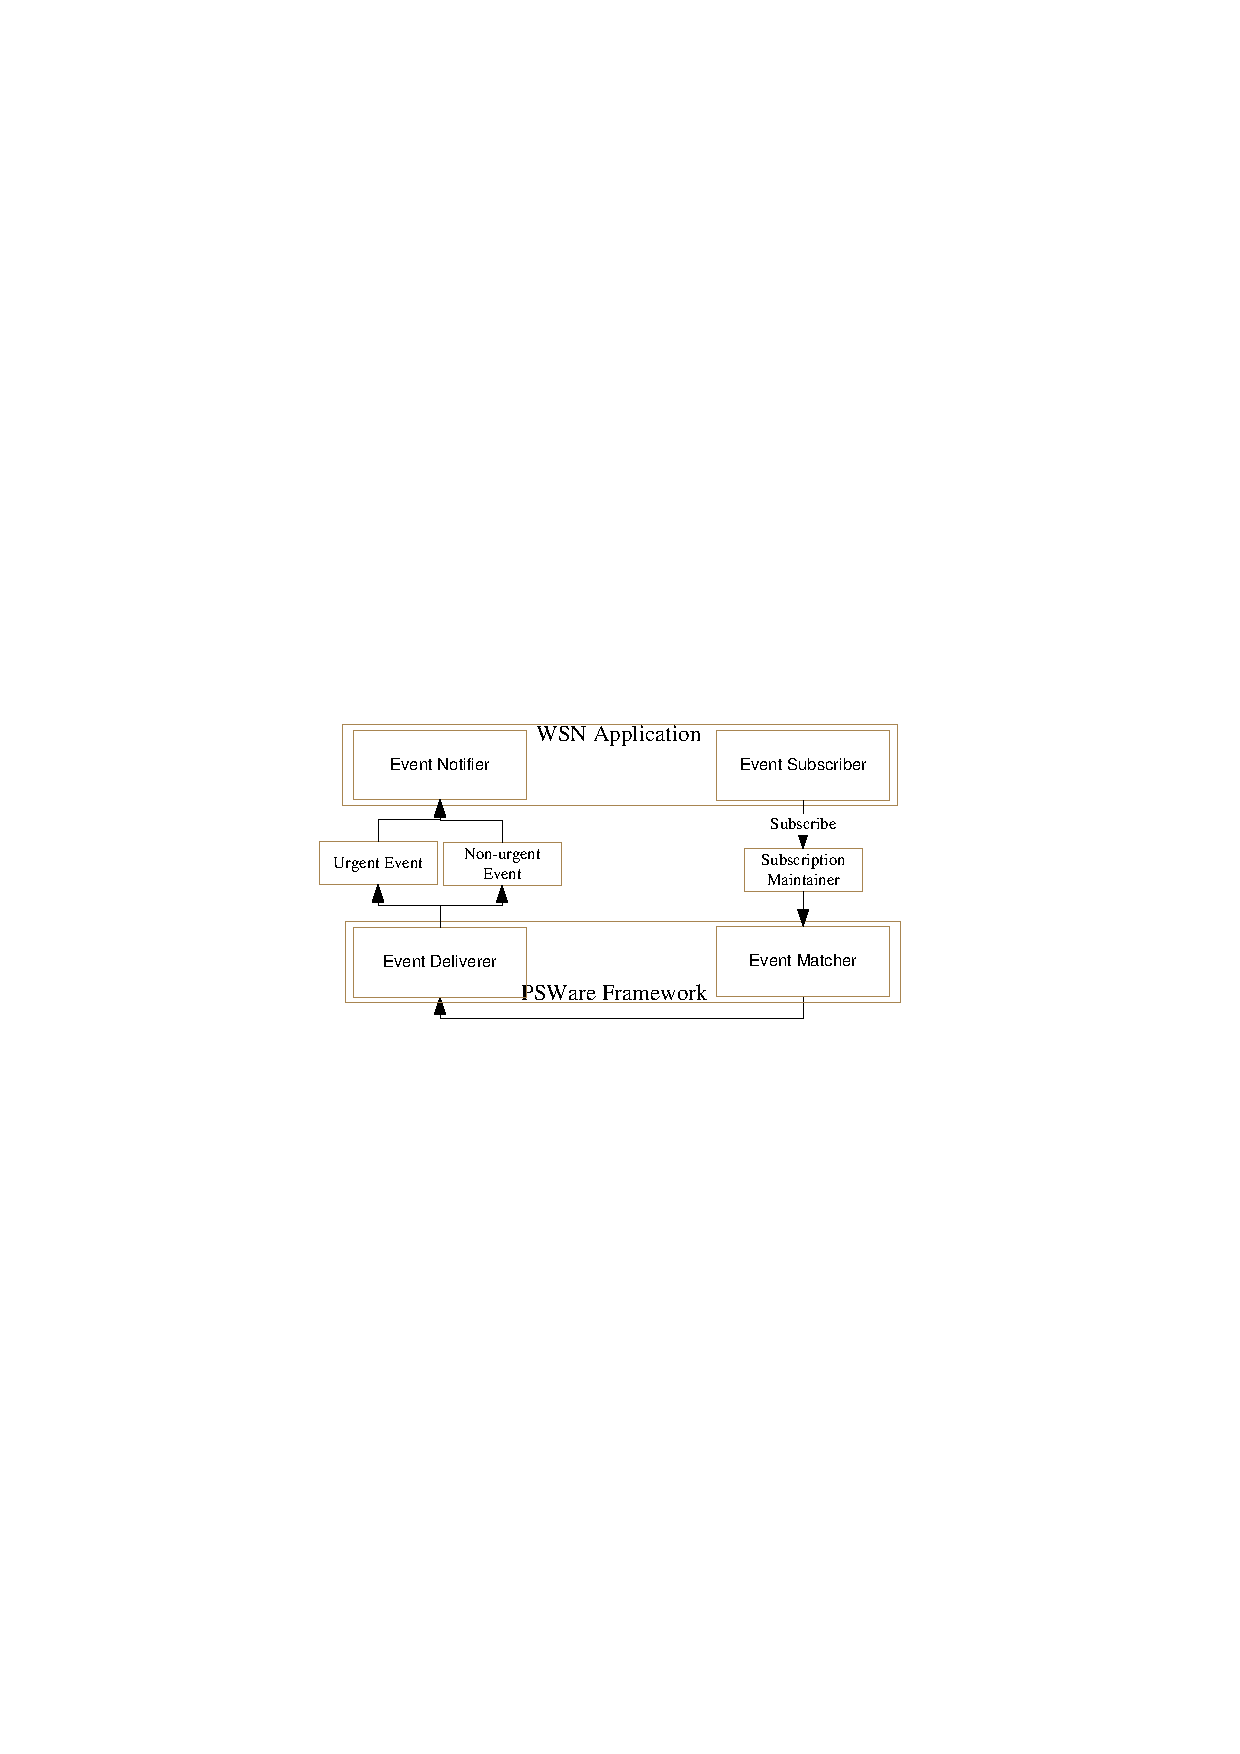
\includegraphics[width=.8\textwidth]{its-delivery}
\caption{Type-based event delivery}
\label{fig:its-delivery}
\end{figure}

The overall architecture for ITS event delivery over PSWare is shown in Figure \ref{fig:its-delivery}. A key difference in this architecture is the introduction of multiple event deliverer. Upon the signaling of 'eventDeliver' in Listing \ref{lst:pswareEventMatcher}, the middleware developer can first query the event type by using the APIs in Listing \ref{lst:pswareAPI}. With 'psware gen', this may be easily achieved. The middlewre just needs to pre-define a domain-specific event type for traffic accident. When events of such types are detected, an emergency delivery method is used. Otherwise, the normal event delivery method will be used.

\cleardoublepage

\floatname{algorithm}{Algorithm}
\chapter{Composite Event Detection}
\label{chapter:ted}
\section{The Composite Event Detection Problem}
\label{sec:system_model}
Event detection algorithm is the heart of a pub/sub system. In this section, we formally define the composite event detection algorithm.

\subsection{System Model}
We consider the network as a graph \(G=(N, A)\) where each node represents a sensor node and each edge represents a communication link. For each \(a_n\in A\), it has a weight \(W_n\) associated with it.

The subscriber provides a finite set of event types \(E=\{e_1,e_2,\cdots\}\). For each \(e_n\in E\), the subscriber defines a set of attributes \(e_n\rightarrow attr_n\) which reflect certain real world phenomenon. 

The subscriber also provides a finite set of event relations \(R=\{r_1,r_2, \cdots\}\) where each \(r_n\in R\) represents the mapping of one or more sub-event types \(e_1, e_2\cdots \in E\) to a composite event type \(e_3\in E\), denoted as \(r_n(e_1, e_2, \cdots)=e_3\). One of the event type \(e_s\in E\) is subscribed by the subscriber. %Event types and their relations can be represented as a directed acyclic graph (DAG) as shown in Figure \ref{fig:eventdag}, where each node represents an event and each edge represents a relation between a sub-event and a composite event.

\begin{comment}
\begin{figure}
\centering
\figurecurrentwidth{eventdag}
\caption{Event DAG}
\label{fig:eventdag}
\end{figure}
\end{comment}

We have a set of primitive event types \(E_{primitive}\subseteq E\) event types such that \(\not{\exists} r_n\in R\) such that \(r_n(e_1, e_2, \cdots)=e_n\) where \(e_n\in E_{primitive}\) and \(e_1, e_2, \cdots \in E\). For each primitive event of type \(e'_n\in E_{primitive}\), it will be detected by a node \(n_i\in N\). We use the message cost as the event detection cost for each event type \(e_n\in E\), denoted as \(cost(e_n)\).

\subsection{Problem Formulation}
Given:
\begin{itemize}
	\item A network \(G=(N, A)\)
	\item A set of event types \(E\) with relation \(R\)
	\item A cost function \(cost(e_n)\) for \(e_n\in E\)
\end{itemize}

Find:
\begin{itemize}
	\item For each event type \(e_n\in E\), when an event instance of this type is happens, find a subset of nodes \(V_n^r\subseteq V\) which are involved in detecting the event.
\end{itemize}

Objective:
\begin{itemize}
	\item Minimize the total energy consumption:
	\begin{displaymath}
	\sum_{i=i}^{n}cost(e_i)
	\end{displaymath}
\end{itemize}

\begin{theorem}
\label{thm:tableConstruction}
The composite event detection problem is NP-complete.
\end{theorem}

\begin{proof}
We show our proof by reducing the steiner tree problem to our composite event detection problem. Let \(N_s\subset N\) be the event source (nodes that detect the primitive events). Since the cost is defined as message cost, if we minimize the total path length from the event sources to the fusion points (nodes which are responsible for detecting composite events), then we can also minimize the message cost.

We construct a graph \(G'=(N', A')\) from \(G\) with the steps as follows:
\begin{enumerate}
\item \(N'=N_s\bigcup N_f\)
\item For each pair of nodes \(n'_i, n'_j\in N'\), we add an edge \(a'_k\in A'\) incident on both if there is a path from \(n'_i\) to \(n'_j\) in \(G\).
\item The weight of the newly added edge is \(a'_k\) is the weight of the shortest path from \(n'_i\) to \(n'_j\) in \(G\).
\end{enumerate}

The corresponding Steiner tree problem can be defined as below.

Given:
\begin{itemize}
\item A graph: \(G'=(N', A')\)
\item Each edge \(e'_i\) in the graph has a weight of \(W'_i\)
\item A set of sources: \(N_s\subset N\)
\end{itemize}

Find:
\begin{itemize}
\item A minimum Steiner tree that spans \(N_s\)
\end{itemize}

If we have a solution for the Steiner tree problem in \(G'\), then we simply need to recover the shortest paths in \(G\) and it will also be the optimal solution for our composite event detection problem. On the other hand, an optimal solution for our composite event detection problem is also an optimal solution for the Steiner tree problem if we replace the paths between every pair of nodes \(n'_i, n'_j\in N'\)  with the edges in \(A'\).
\end{proof}

\section{A Centralized Approach}
\label{sec:centralized}
Based on our problem formulation, we can intuitively use a centralized approach to solve this problem. In the centralized approach, when the sensor nodes detect the events, they first inform the sink node about the detected event. Then the sink node will select the efficient nodes as event fusion points for each event type and broadcast the information into the network. The nodes will then forward their events to these fusion points. The fusion points may be changed or updated with a predetermined probability to cope with event dynamics. The reasons why the nodes will only inform the sink about the events they detected rather than send the events to the sink for detection are as follows:
\begin{itemize}
\item Each individual event may have a lot of attributes so it is more desirable to first calculate the energy-efficient event fusion points before the actual event detection.
\item As described in Section \ref{sec:introduction}, events may have strong locality. Therefore, the fusion points selected may be used for detecting events of the same types in the future.
\end{itemize}

We assume the users have no prior knowledge on where the events might happen. However, they do know the probability distribution of the events. We will discuss the event probability distribution and its impact on the algorithm in the latter section when we describe how the algorithm is designed to cope with event dynamics.

The input of the algorithm includes:
\begin{itemize}
\item Sensor network: \(G\)
\item A set of events \(E'=\{e_i^1, e_i^2, \cdots \}\) where \(e_i^j\) denotes an event of type \(e_i\)
\end{itemize}

\begin{algorithm}
\begin{algorithmic}[1]
\REQUIRE \(G=(N,A)\), \(E'\)
	\FORALL {\(e_i^j\in E'\)}
		\IF {\(e_i\) is not assigned to any node}
			\STATE Find any other \(e_k^l\in E'\) such that either k==i or \(e_k\) and \(e_i\) has a relation for a composite event \(e_x\)
			\FORALL {\(n \in N\)}
				\STATE Construct an SPT for all \(e_k^l\) and \(e_i^j\) with root as \(n\)
				\STATE Calculate the cost for the SPT as \(cost_n\)
			\ENDFOR
			\STATE Find the SPT with the smallest \(cost_n\) and select \(n\) as fusion point for \(e_k\) and \(e_i\)
			\STATE Add \(n\) as the node detecting \(e_x^1\) to \(E'\)
		\ENDIF
	\ENDFOR
\end{algorithmic}
\caption{Centralized TED}
\label{algo:centralizedTED}
\end{algorithm}

The algorithm will examine all the primitive events reported from the network to see if there is any relation associated with them. If so, the algorithm will try each node in \(G\) to construct shortest path tree (SPT) for these related events and select the one with the smallest cost. The root of that SPT will then become the fusion point for the related events. The algorithm runs recursively in the sense that once the fusion points for a composite event is selected, itself will become the node for detecting that composite event.

\subsection{Determine the Re-selection Probability}
While the previous section outlines the algorithm for centralized TED, we still need to decide how often the nodes should switch to another fusion point in order to cope with the event dynamics. We use exponential distribution as the event probability distribution because of its memoryless property. More specifically, for each composite event, the distance between each of its sub-events to any point in the network follows an exponential distribution as follows:
\begin{displaymath}
f(x)={\lambda}_1e^{-{\lambda}_1x}
\end{displaymath}

In addition to the distance between events, the direction of events that happen in different rounds will also affect the selection probability. The angle between any pair of related events also satisfy an exponential distribution as follows:
\begin{displaymath}
f(\theta)={\lambda}_2e^{-{\lambda}_2\theta}
\end{displaymath}

Both \(x\) and \(\theta\) are shown in Figure \ref{fig:fp-dist} where the events \(e_1\), \(e_2\) are detected before and \(e'_1\), \(e'_2\) are detected. For simplicity, we use distance to measure the cost for one node to reach another. Let \(d\) be the average distance between any point in the deployment region to the closest sensor node. As shown in Figure \ref{fig:fp-dist}, for a composite event that has two sub-events, originally the event is fused at \(n_1\). Then, for the next detection of \(e'_1\) and \(e'_2\), if the fusion point is still the original one, then the cost will be no less than:
\begin{align*}
cost_1=\sqrt{({\lambda}_1)^2+(\frac{{\lambda}_1}{2})^2+({\lambda}_1)^2cos(\frac{\pi+{\lambda}_2}{2})}
\end{align*}
On the other hand, if a new fusion point is selected, then the cost will be no more than:
\begin{align*}
cost_2=&2(\frac{{\lambda}_1}{2sin\frac{{\lambda}_2}{2}}+{\lambda}_1)sin\frac{{\lambda}_2}{2}+d\\
=&{\lambda}_1(1+2sin\frac{{\lambda}_2}{2})+d
\end{align*}

\begin{figure}
\centering
\subfloat[Event distribution]{\label{fig:event-distribution1}\figurehalfwidth{event-distribution1}}
\subfloat[Fusion point distance]{\label{fig:fp-dist}\figurehalfwidth{fp-dist}}
\caption{Selecting fusion points in centralized approach}
\label{fig:centralizedTED}
\end{figure}

The condition to select a new fusion point will be:
\begin{align}
&cost_1\geq cost_2\nonumber \\
&cost_1^2\geq cost_2^2\nonumber \\
&({\lambda}_1)^2(\frac{5}{4}+cos(\frac{\pi+{\lambda}_2}{2}))\geq\nonumber \\ &{\lambda}_1^2(1+2sin\frac{{\lambda}_2}{2})^2+d^2+2{\lambda}_1(1+2sin\frac{{\lambda}_2}{2})d
\label{eq:fpSwitch}
\end{align}

Here \(d\) is decided by the node density and can be estimated once we know the deployment area and the number of nodes in the deployment area. Therefore, given \(f(x)\), \(f(\theta)\) and \(d\), we can use generalized gradient search to find the values for \(\theta\) and \(x\) such that Equation \ref{eq:fpSwitch} is satisfied while minimizing the probability for switching:
\begin{align*}
P_{switch}&=F(x>x*)F(\theta>\theta *)\\
&=\int_{x*}^{\infty}{\lambda}_1e^{-{\lambda}_1x}dx\int_{\theta *}^{\infty}{\lambda}_2e^{-{\lambda}_2\theta}d\theta\\
&=e^{-{\lambda}_1x*}e^{-{\lambda}_2\theta *}
\end{align*}

Once the probability is obtained, after each event detection, there will be a probability of \(P_{switch}\) that the event will switch to another fusion point. This is done by making the fusion point broadcast a message in the network so that all nodes can delete the corresponding event type assignment to that fusion point.

So far the calculation for \(P_{switch}\) is based on the assumption that the network scale is not known in advance and the cost for broadcasting new fusion point information is not known in advance. If the network scale is known to be \(|N|\) in advance, then we can change Equation \ref{eq:fpSwitch} a bit to be more accurate as in Equation \ref{eq:fpSwitchAccruate}.

\begin{align}
cost_1\geq cost_2+|N|\times P_{switch}
\label{eq:fpSwitchAccruate}
\end{align}

By calculating \(|N|\times P_{switch}\), we can further fine-tune the switching probability to balance with the broadcast cost.
\section{TED: a Type-based Event Detection Algorithm}
\label{sec:ted}
In this section, we propose TED, a distributed type-based composite event detection algorithm for WSN. The essential idea of TED is that after each sub-event is detected, the nodes will at first forward the detected events randomly to some nearby fusion points in the hope that at least some of them will be good ones. When the composite events are detected, the fusion points will first check the record to see if the source nodes have already selected any fusion point. If not, it will flood some feedback in the network so that the source node will get it and other nodes can also use such feedbacks as 'hints' when they need to forward the events. By collecting different feedbacks from different fusion points, the sensor nodes will choose the best one according to the cost. If the sub-events occur again, the nodes will be able to forward the detected events based on the feedback so that the cost could likely be reduced.

\subsection{Algorithm Input}
In TED, the set of event fusion points \(N_f\subseteq N\) are preselected. We will discuss how to select the fusion points in an optimal way in the latter part of the section. Therefore, each node will play two possible roles: normal node or event fusion point. Normal nodes will need the following data structure for the algorithm:
\begin{itemize}
\item Event filter table \(table_f\): this table stores the filters for each event type. \(table_f\rightarrow filter_n\) denotes the filter for event type \(e_n\).
\item Fusion point routing table (\(table_r\)): this table defines the routing to each fusion point \(n_i\in N_f\). \(table_r\rightarrow n_i\rightarrow parent\) denotes the parent node to reach fusion point \(n_i\).
\item Event forwarding table (\(table_e\)): this table defines for each event type \(e_n\in E\), the corresponding fusion point for the it. \(table_e\rightarrow e_n\rightarrow fp\) denotes the fusion point for event type \(e_n\).
\end{itemize}

The fusion points will also have the same data structure of the normal nodes for the algorithm. In addition, they will have an additional table \(table_m\). This table temporarily stores the events collected from other nodes. For each of the entries it has the following contents: 
\begin{itemize}
\item \(e^i_n\): the \(i^{th}\) event of type \(e_n\)
\item \(cost\): the detection cost for the event \(e^i_n\)
\item \(flag\): the flag (to be described in the algorithms) for the event \(e^i_n\)
\end{itemize}

\subsection{TED for Normal Nodes}
Since the event detection starts from primitive events, the normal nodes will run Algorithm \ref{algo:normalNode} after detecting a primitive event \(e^i_n\) of type \(e_n\).
\begin{algorithm}
\begin{algorithmic}[1]
\REQUIRE evaluate(\(e^i_n\), \(table_f\rightarrow filter_n\))==True
	\IF {\(table_e\rightarrow e_n\rightarrow flag\neq fpUnknown\)}
		\STATE \(toForward=table_e\rightarrow e_n\rightarrow fp\)
		\STATE Set \(e^i_n\rightarrow flag=table_e\rightarrow e_n\rightarrow flag\)
		\STATE Forward \(e^i_n\) to \(table_r\rightarrow fp\rightarrow parent\)
	\ELSE
		\IF{\(table_e\rightarrow e_n\rightarrow flag\neq fpUnknown\)}
			\STATE Select \(k-1\) nearest fusion points \(N_k\in N_f\)
			\STATE \(N_k=N_k\bigcup \{table_e\rightarrow e_n\rightarrow fp\}\)
		\ELSE
			\STATE Select \(k\) nearest fusion points \(N_k\in N_f\)
		\ENDIF
		\FOR {each \(n\in N_k\)}
			\STATE forward \(e^i_n\) to \(table_r\rightarrow n\rightarrow parent\)
		\ENDFOR
	\ENDIF
	
	\IF {\(e^i_n\rightarrow flag=fpSelected\) \AND \(e^i_n\rightarrow timeout==True\)}
		\STATE \(table_e\rightarrow e_n\rightarrow flag=fpIndicated\)
	\ENDIF
\REQUIRE feedback of event type \(e_n\) from \(n_i\in N_f\)
	\STATE \(entry=table_e\rightarrow e_n\)
	\IF {\(e_n\rightarrow source==self\) \AND (\(entry\rightarrow flag\neq fpSelected\) \OR \(entry\rightarrow flag==fpSelected\) \AND \(entry\rightarrow cost<e_n\rightarrow cost\))}
		\STATE \(entry\rightarrow flag=fpSelected\)
		\STATE \(entry\rightarrow fp=n_i\)
	\ELSIF {\(entry\rightarrow cost<e_n\rightarrow cost\)}
		\STATE \(table_e\rightarrow e_n\rightarrow flag=fpIndicated\)
	\ENDIF
\end{algorithmic}
\caption{TED for normal nodes}
\label{algo:normalNode}
\end{algorithm}
For each event type, it has three possible states: fpUnknown, fpIndicated and fpSelected. Initially, all the event types are fpUnknown because the sensor node does not know which fusion point is the best to forward the event. The flag will be updated upon the reception of feedbacks from the fusion points. More specifically, if the event is detected at the fusion point \(n_i\), the fusion point will flood the feedback with cost and event source included so that the nodes can update their corresponding flags. The update is based on the detection cost.

Upon the detection of event \(e^i_n\), the node will first check if there is already a fusion point assigned to it. If so, the event will simply be forwarded to that fusion point. Otherwise, the node will choose \(k\) closest fusion points randomly and then forward the events to them.

\subsection{TED for Event Fusion Points}
When the fusion point receives \(e^i_n\) from a node, it will first wait a period of time until the expiry time of the event to check for other events for possible matches. If no match is found during this period, the fusion point will still use Algorithm \ref{algo:normalNode} to further forward the events to other fusion points. The pseudo code is shown in Algorithm \ref{algo:fusionPoint}.

\begin{algorithm}
\begin{algorithmic}[1]
\REQUIRE \(e^i_n\) from node \(n_i\in N\)
	\FORALL {\(e_j\in E\)}
		\IF {\(e_n\) is a subevent of \(e_j\)}
			\STATE result = evaluate \(e_j\) with \(e^i_n\)
			\IF {result==True}
				\STATE detected (\(e_j\))
				\STATE \(e_j\rightarrow cost=e_j\rightarrow cost+e^i_n\rightarrow cost\)
				\STATE \(e_j\rightarrow source=e_j\rightarrow source\bigcup e^i_n\rightarrow source\)
				\STATE feedback (\(e_j\))
			\ENDIF
		\ENDIF
	\ENDFOR
\REQUIRE expiry time of \(e^i_n\)
	\STATE detected (\(e_j\))
\end{algorithmic}
\caption{TED for fusion points}
\label{algo:fusionPoint}
\end{algorithm}

The function 'detected' is the place where Algorithm \ref{algo:normalNode} is invoked. Upon the detection of any composite event, the fusion point will also send the feedbacks to the network.


\section{Fusion Point Deployment Problem}
Because our distributed algorithm is based on certain nodes in the network that acts as event fusion points to detect the events, in this section, we discuss how to select such fusion points in order to optimally detect the events.
\subsection{Even Deployment}
We first look at a deployment where fusion points are evenly deployed. We use the following deployment model:
\begin{itemize}
\item The entire network is divided into a set of equally sized regions.
\item Within each region, we deploy the same number of event fusion points. 
\end{itemize}

Such deployment model is suitable if the user has no prior knowledge on where events would happen. After calculating the optimal deployment strategy, the users can make use of it in two ways:
\begin{itemize}
\item After the sensor deployment, the users can deploy additional sensor nodes as fusion points in the network.
\item Before the deployment, the user can calculate how many fusion points are needed in the network and mix them with normal nodes to deploy them randomly.
\end{itemize}
We will use square for calculating the optimal deployment strategy in this work. The optimal deployment strategies with regions of other types of shape may be also be obtained in a similar fashion. Suppose we divide the whole region of area \(A\) into squares of size \(s\times s\). Then on average, each sensor node can find a fusion point at a distance of \cite{vertexDistance}:
\begin{align}
r=&\int_0^1D(t)dt\nonumber\\
=&\int_0^1\frac{2}{3}\sqrt{c^2t^2+(b^2-a^2-c^2)t+a^2}dt\nonumber\\
=&\frac{c}{6}[u(1+v^2)+\frac{1}{2}(1-u^2)(1-v^2)ln(\frac{u-1}{u+1})]\label{eq:avgdist1}
\end{align}
where,
\begin{align}
c=&\frac{s}{2}\nonumber\\
u=&\frac{\sqrt{2}+1}{2}s\nonumber\\
v=&\frac{\sqrt{2}-1}{2}s\label{eq:avgdist2}
\end{align}

In order to determine the optimal deployment strategy, we also need to know the event probabilistic distribution. We use the same exponential distribution model as introduced in Section \ref{sec:centralized}. %We start by considering the simplest case where two sub-event types \(e_1\) and \(e_2\) form a composite event type \(e_3\) (\(r_n(e_1, e_2)=e_3\)). 

The cost introduced by TED mainly consists of three parts: forwarding cost, feedback cost and detection cost. Initially, upon the detection of primitive events, the nodes will randomly forward the events to \(k\) closest fusion points. 
\begin{displaymath}
cost_{forward}=r\times k
\end{displaymath}

Here \(k\) is determined by the event distribution such that after forwarding different sub-events to the fusion points, there will be some overlapping fusion points for different sub-events. Therefore, \(k\) is defined as follows:
\begin{equation}
k=(\frac{{\lambda}_1}{r}+1)^2\label{eq:forwardNum}
\end{equation}

When the events are detected at the fusion points, feedback will be sent to the event sources so that the sensor nodes can later forward the events to them and the cost will be reduced. For simplicity of analysis, we assume the fusion points will simply flood the feedback in the network. Therefore, the feedback cost is:
\begin{displaymath}
cost_{feedback}=|N|\times k
\end{displaymath}

The detection cost is the message cost for all sub-events to be forwarded to a fusion point so that the composite event may be detected. As shown in Figure \ref{fig:cedu-detectionCost}, if we have two events \(e_1\) and \(e_2\), the minimum event detection cost will be detecting the events on the line segment that connects the two events. However, we may not find a fusion point on the line segment, so in order to find a fusion point that can minimize energy cost, we should choose a point that lies on the center of the line segment. Similar to Equation \ref{eq:avgdist1} and \ref{eq:avgdist2}, the average detection cost will be:
\begin{displaymath}
cost_{detect}=2\times \int_0^{arctan\frac{2r}{{\lambda}_1}}\frac{{\lambda}_1}{2cosx}dx
\end{displaymath}

\begin{figure}
\centering
\figurecurrentwidth{cedu-detectionCost}
\caption{Event detection cost}
\label{fig:cedu-detectionCost}
\end{figure}

Since each node needs to know how to reach the fusion points when forwarding is needed, there is overhead for maintaining such information. Similar to many existing routing protocols for WSN, we assume the nodes will periodically send messages for link evaluation \cite{rssiroute}. Therefore, the cost for maintenance is:
\begin{displaymath}
cost_{maintenance}=(\frac{A}{s^2})|N|c_1
\end{displaymath}

Here, \(c_1\) is constant that represents the relation between energy consumption and the size of the packets. In addition, the sensor node should also have storage constraint because the nodes simply might not able to store all the routes to every fusion point. The storage constraint is defined as:
\begin{displaymath}
(\frac{A}{s^2})<c_2
\end{displaymath}

Objective is to minimize:
\begin{displaymath}
cost_{all}=2(\frac{T}{t}+1)cost_{forward}+cost_{maintenance}+Tcost_{detect}
\end{displaymath}

All the constants are summarized in Table \ref{tab:ceduConstants}. \(cost_{all}\) may be obtained by nonlinear programming techniques such as generalized gradient search algorithm. In addition to square deployment, other deployment method may also be used and the only difference lies in Equation \ref{eq:avgdist1}, \ref{eq:avgdist2} and \ref{eq:forwardNum}.

\begin{table}
\begin{center}
\begin{tabular}{ | p{1cm} | p{5cm} | }
\hline
\({\lambda}_1\) & Expected location between the events \\ \hline
\({\lambda}_2\) & Expected angle of the events \\ \hline
\(A\) & Deployment area \\ \hline
\(s\times s\) & The size of the square sub-regions \\ \hline
\(c_1\) & Energy cost per bit of data transmission\\ \hline
\(c_2\) & Storage constraint\\ \hline
\end{tabular}
\end{center}
\caption{Summary of the symbols in TED}
\label{tab:ceduConstants}
\end{table}

\subsection{Hierarchical Deployment}
Apart from even deployment, the fusion points may also be deployed in a hierarchical fashion. Formally, we assume a square network deployment where the fusion points are distributed in a hierarchical way in the network. We assume that the sink node is at the center of the network. And more fusion points can be added by dividing the network evenly into the square sub-regions of same size. For example, a network with only sink node is shown in Figure \ref{fig:fplvl1}. If we add 4 fusion points, the fusion points will be evenly distributed in the network as in Figure \ref{fig:fplvl2}.

We can achieve flexibility with this distribution model since we can add more fusion nodes into the network if we want to decrease the cost for detecting composite events.

\begin{figure}
\centering
\subfloat[Level 1 fusion point]{\label{fig:fplvl1}\figurehalfwidth{fplvl1}}
\subfloat[Level 2 fusion points]{\label{fig:fplvl2}\figurehalfwidth{fplvl2}}
\caption{Fusion point distribution model in TED}
\label{fig:fplvl1-2}
\end{figure}

For fusion level at \(i\)th level, the whole network is divided into \(2^{i-1}\) subregions \(region_i\). For example, if the fusion level is at \(1\) as shown in Figure \ref{fig:fplvl1}, the region covers the entire network. In Figure \ref{fig:fplvl2}, the network is divided into \(4\) subregions at fusion level \(2\).

In our analytical model, we assume dynamic events where for each event type \(e_n\), it may occur anywhere in the network. In order to include such kind of properties in the model, we define for each \(e_n \in E\), it will be monitored by \(t\) rounds. The interval between the rounds are \(T_n\). During this \(t\times T_n\) time, the set of detected events of type \(e_n\) is defined as \(E_n=\{e_n^1, e_n^2, \cdots e_n^t\}\).

We measure the event detection cost in terms of message cost. For simplicity, we measure the message cost by the distance (which will in term be reflected as the number of hops) a node can reach another. We uses shortest path tree (SPT) data aggregation protocol \cite{impactaggregation} as reference to see under what conditions TED can outperform data aggregation protocols which do consider event relations.

When the fusion points are hierarchically distributed in the network, the composite event detection cost will be bounded by the level of fusion points distributed in the network. Consider Figure \ref{fig:fpdistribution} as an example, if we have a sensor network in a rectangular region where it can be further be divided into two smaller square region. If we assume for each square region, the diameter length is \(d\), then in Figure \ref{fig:evendistribution}, if we evenly distribute a fusion point in each square region, the max distance for any sensor node in the whole network to reach it's closest fusion point is \(\frac{d}{2}\). If the fusion points aren't evenly distributed as shown in Figure \ref{fig:unevendistribution}, then for some nodes in the network, it might have a distance larger than \(\frac{d}{2}\) to reach the fusion point.

\begin{figure}
\centering
\subfloat[Even distribution]{\label{fig:evendistribution}\figurehalfwidth{evendistribution}}
\subfloat[Uneven distribution]{\label{fig:unevendistribution}\figurehalfwidth{unevendistribution}}
\caption{Fusion point distribution}
\label{fig:fpdistribution}
\end{figure}

\begin{theorem}
\label{thm:evenfp}
Let the network diameter be \(d\), and the fusion point level be \(l\), the distance between two sub-events \(e_1\) and \(e_2\) is \(r\). After \(e_1\) and \(e_2\) have already been detected, the upper bound of the energy cost for detecting the composite event \(e_3\) based on \(e_1\) and \(e_2\) is:
\[
cost(e_3)=\frac{d}{2^{l-1}}+r
\]
\end{theorem}

\begin{proof}
As shown in Figure \ref{fig:evendistribution}, the upper bound for one single event to reach a fusion point is:
\begin{displaymath}
\frac{d}{2^{l}}
\end{displaymath}
Then, the upper bound on the cost for the the two fusion points to reach each other is:
\begin{displaymath}
\frac{d}{2^{l-1}}+r
\end{displaymath}
\end{proof}

Theorem \ref{thm:evenfp} indicates that if we have no prior knowledge about the events to happen in the network, then fusion points with even distribution can still allow us to have an upper bound on the composite event detection cost.

\begin{theorem}
\label{thm:fpdistance}
If a node is a level \(l\) fusion point, then its distance from sink \(r \in D_l\)
\[
D_l=\{a_1, a_2, \cdots a_{2^{l-2}}|a_i=\frac{d}{2^{l-1}} \times (2i-1),i<2^{l-2}\}
\]
\end{theorem}
\begin{proof}
When \(l=1\), only sink node is the fusion point. Hence \(D_1=\{0\}\). Similarly, when \(l=2\), \(D_2=\{\frac{d}{2}\}\). We denote each \(a_i \in D_k\) as \(a_i^k\). Based on our fusion point distribution scheme, at fusion level \(k+1\), we simply divide the sub-regions at fusion level \(k\) into four. Therefore, for each \(a_i^k \in D_k\), we can find two elements \(a_{2i-1}^{k+1}, a_{2i}^{k+1} \in D_{k+1}\) such that:
\begin{align*}
&\left\{
\begin{array}{l}
a_{2i-1}^{k+1}=a_i^k-\frac{d}{2^k}\\
a_{2i}^{k+1}=a_i^k+\frac{d}{2^k}
\end{array}
\right.\\
\Rightarrow
&\left\{
\begin{array}{l}
a_{2i-1}^{k+1}=\frac{d}{2^{k-1}} \times (2i-1)-\frac{d}{2^k}\\
a_{2i}^{k+1}=\frac{d}{2^{k-1}} \times (2i-1)+\frac{d}{2^k}
\end{array}
\right.\\
\Rightarrow
&\left\{
\begin{array}{l}
a_{2i-1}^{k+1}=\frac{d}{2^{k}} \times (2(2i-1)+1)\\
a_{2i}^{k+1}=\frac{d}{2^{k}} \times (2(2i)+1)
\end{array}
\right.
\end{align*}

Hence, Theorem \ref{thm:fpdistance} holds for any natural number.
\end{proof}

Theorem \ref{thm:fpdistance} may be used as one of the conditions for selecting fusion points.
\cleardoublepage

\chapter{Clustering for PSWare}
\label{chapter:clustering}
In the previous chapter, we outline TED, a distributed event detection algorithm. In addition, we describe a hierarchical fusion point placement problem. However, these algorithms use generic event probabilistic model and may not perform well compared with more application specific algorithms. Fortunately, PSWare has the flexibility of incorporating different algorithms. In this chapter, motivated by SHM application we describe a novel clustering algorithm that can help to detect events in this application domain.

\section{Overview of WSN-based SHM}
One potential application of WSNs that is far less investigated by computer science researchers is structural health monitoring (SHM).  The objective of SHM is to monitor the integrity of structures such as buildings, dams, bridges, and to detect and pinpoint the locations of any possible damage. Unlike other monitoring applications, detection of possible structure damage is not straightforward and requires significant amount of domain knowledge such as finite element model updating and damage indicator extraction \cite{farrar2007introduction}. Moreover, many assumptions which were used to model the network associated problems, such as unit disk or convex sensing region, 0/1 local decision, or data aggregation by average, are unfortunately not realistic in SHM.  The required domain knowledge, along with the complexity of SHM, prohibits computer science researchers from investigating this application as intensely as others.

As a result, most research work so far in WSN-based SHM was done by researchers in civil engineering.  Using their knowledge in structure engineering, they have designed and developed many WSN-based SHM systems \cite{lynch2003embedment}\cite{nagayama2008structural}. However, based on our experience obtained from the previous collaborations with civil researchers, they generally concern whether the developed WSN-based SHM system can replicate the data delivery functionality of original wire-based counterpart and have less interest to embed in-network processing technology. Moreover, although they have solved many practical engineering problems, they still have difficulties to handle limitations of WSNs such as limited wireless bandwidth, limited communication range, and limited resources of wireless sensor nodes, etc.  When designing WSN-based SHM systems, civil engineers sometimes choose powerful wireless sensor nodes to accomplish work that could have been achieved by more cost-effective counterpart through system optimization. This leaves a large space to explore for computer science researchers.

We demonstrate that computer science researchers can help fill this gap and significantly improve the performance of a WSN-based SHM system. We consider a fundamental problem in SHM: modal analysis, by which the vibrational characteristics of a structure are obtained.  These characteristics, called modal parameters, are basis for most of SHM algorithms and can also be used for vibration control and safety assessment. Traditional modal analysis is centralized which needs to stream all the measurement data back to a central unit. This method generally has high energy consumption and low scalability. We describe a cluster-based modal analysis approach. The basic idea of this approach is similar like the 'divide and conquer', where sensor nodes deployed on a structure are partitioned into clusters and modal analysis is carried out in each cluster. The resultant modal parameters of each cluster are then assembled together to obtain the modal parameters of the whole structure. In this approach, clustering is of great importance and should meet some extra requirements of modal analysis. Moreover, cluster size should be optimized to minimize the total energy consumption.

The outline for the rest sections in this chapter is as follows:
\begin{enumerate}
\item	We show that design of a WSN-based SHM system is a multi-disciplinary area that the efforts from researchers in computer science engineering can significantly help improve system's usability and efficiency. 
\item We proposed a cluster-based modal analysis strategy. The clustering problem in this strategy is formulated and proven to be NP-complete.  Two centralized and one distributed algorithms are proposed.
\end{enumerate}

\section{Structural Mode Shapes}
In this section, we will describe the cluster-based modal analysis approach with focus on the optimization of clustering. Before we formulate this clustering problem, the basic concept of modal parameters, the techniques adopted for modal analysis and assembling method are described. Table \ref{tab:Table1} summarizes the notations to be used.

\begin{table}
	\centering
\begin{tabular}{|c|l|}
\hline
\(\mathbf{\Psi_k}\)& The \(k^{th}\) mode shape vector of the structure\\
\hline
\(p\) &	The number of mode shape vectors to be identified\\
\hline
\(G_{xy}(\omega)\)& The cross spectral density (\(x\neq y\))\\
\ & and power spectral density (\(x=y\))\\
\hline
\(N\) & the total data amount\\
\hline
\(M,c,n_i\) & the total number of sensor nodes,\\ 
\ & the number of generated clusters, \\
\ & and the number of sensor nodes in cluster \(S_i\)\\
\hline
\(n_t\)	& Length of each section to calculate CSD\\
\hline
\(n_d\)	& Number of averages\\
\hline
\(e_S, e_R, e_T \)& Energy consumed for sampling/rece./trans. one data\\
\hline
\(e_{NExT}, e_{ERA}\)	& Energy consumed for NExT and ERA\\
\hline
\end{tabular}
	\caption{Summary of Notations}
	\label{tab:Table1}
\end{table}

In particular, we give a brief introduction of one important type of modal parameters: mode shapes. 

Each mechanical structure has a number of specific vibration patterns at specific frequencies. These vibration patterns are called mode shapes. For example, we deploy a total of \(m\) sensor nodes on a structure and extract a total of \(p\) mode shapes from the measurement of these sensors:

\begin{equation}
[\mathbf{\Psi_1}, \mathbf{\Psi_2}, \cdots, \mathbf{\Psi_p}]=
\begin{bmatrix}
\phi_{11} & \phi_{12} & \cdots & \phi_{1p}\\
\phi_{21} & \phi_{22} & \cdots & \phi_{2p}\\
\vdots  & \vdots  & \ddots & \vdots  \\
\phi_{m1} & \phi_{m2} & \cdots & \phi_{mp}
\end{bmatrix} 
\end{equation}
where mode shape \(\mathbf{\Psi_k}=[\phi_{1k}, \phi_{2k}, \cdots, \phi_{mk}]'\) is the \(k^{th}\) vibration pattern of the structure.  \(\phi_{ik}(i=1,2,\cdots ,m)\) is the \(k^{th}\) mode shape value defined at the \(i^{th}\) sensor.

As an example, Figure \ref{fig:modes} illustrates the first three mode shapes of a typical cantilevered beam, extracted from the measurements of the deployed 12 sensor nodes. Figure \ref{fig:originalbeam} represents the Original beam. Figure \ref{fig:mode1}, \ref{fig:mode2} and \ref{fig:mode3} represents Mode Shape 1, Mode Shape 2 and Mode Shape 3 respectively.

\begin{figure}
\centering
\subfloat[]{\label{fig:originalbeam}
%\figurecurrentwidth{originalbeam}}
\figurehalfwidth{originalbeam}}
%\qquad
\subfloat[]{\label{fig:mode1}
%\figurecurrentwidth{mode1}}
\figurehalfwidth{mode1}}
\qquad
\subfloat[]{\label{fig:mode2}
%\figurecurrentwidth{mode2}}
\figurehalfwidth{mode2}}
%\qquad
\subfloat[]{\label{fig:mode3}
%\figurecurrentwidth{mode3}}
\figurehalfwidth{mode3}}
%\qquad
%\subfloat[Mode 4 (Freq.=30.8Hz)]{\label{fig:mode4}
%\figurecurrentwidth{mode4}}
%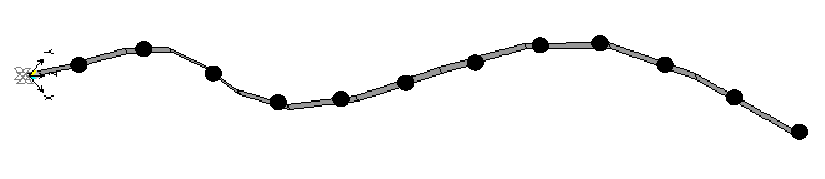
\includegraphics[width=.49\textwidth, height=0.05\textwidth]{mode4}}
\caption{Mode shapes of a typical cantilevered beam}
\label{fig:modes}
\end{figure}

It can be seen that mode shape vector \(\mathbf{\Psi_k}\) has an element corresponding to each sensor node. The more number of sensor nodes used, the more elements are contained in \(\mathbf{\Psi_k}\), and more accurately this vibration pattern of the structure is described. Considering example in Figure \ref{fig:modes}, if we double the number of nodes deployed on the beam, the vibration patterns will be represented with higher granularity. Another important characteristic of mode shape is that elements in \(\mathbf{\Psi_k}\) only represent the relative vibration amplitudes of structure at corresponding sensor nodes. That is, \(\mathbf{\Psi_k}=\zeta \mathbf{\Psi_k}\), where \(\zeta\) is any non-zero real number. This property will be re-visited when we formulate the clustering problem in section \ref{sec:OptimalClustering}.
\subsection{Clustering for Modal Analysis}
In this sub-section, we first give an overview of this cluster-based approach and then formulate the energy consumption of cluster-based modal analysis.

In the cluster-based modal analysis, deployed sensor nodes are partitioned into a number of single-hop clusters and each CH performs intra-cluster modal analysis to extract local mode shapes. Since mode shapes of a cluster only contain elements corresponding to the sensor nodes in that cluster, the mode shapes in all the clusters need to be assembled to obtain the mode shapes defined on all the deployed sensor nodes. The whole process is illustrated in Figure \ref{fig:clusterflow}.

\begin{figure}
	\centering
		\figurecurrentwidth{clusterflow}
	\caption{Overview of cluster-based modal analysis process}
	\label{fig:clusterflow}
\end{figure}

The modal parameters are identified using the natural excitation technique (NExT)\cite{james1993natural} in conjunction with the ERA. NexT+ERA is a widely accepted modal analysis approach and can give accurate mode shape estimate using output data-only. 

In each cluster, the NExT is used first to calculate power spectral density (PSD) of the CH and cross spectral density (CSD) between the CH and each of the cluster member. PSD and CSD functions are estimated using:
\begin{equation}
G_{xy}(\omega)=\frac{1}{n_d\cdot n_t}\sum\limits_{i=1}^{n_d}X_i^*(\omega)\cdot Y_i(\omega) \label{eq:next}
\end{equation}
where \(G_{xy}(\omega)\) is the CSD between two vibration signals, \(x(t)\) and \(y(t)\), measured from CH and a cluster member, respectively. \(X(\omega)\) and \(Y(\omega)\) are the Fourier transforms of \(x(t)\) and \(y(t)\), and '*' denotes the complex conjugate. \(n_t\) is time length of each record \(x_i(t)\) or \(y_i(t)\). \(n_d\) is the number of averages mainly for denoising purpose and \(n_d\) practically ranges from 10 to 20. When calculating \(G_{xy}\), consecutive records of \(x_i(t)\)(also \(y_i(t)\)) generally overlap. When \(y(t)\) in Eq. \ref{eq:next} is replace by \(x(t)\), the power spectral density (PSD) of CH is obtained. 

After obtaining CSD and PSD functions, the inverse Fourier transform is implemented and the cross-correlation functions (CCFs) and auto-correlation function (ACF) are obtained.  The ERA uses these functions to build a state space system whereby mode shapes of the structure are identified.

Traditionally, CH collects the raw data from all its cluster members, calculates CSDs and its PSD, and then uses the ERA to identify mode shapes.  However, the model-based data aggregation method proposed by \cite{nagayama2008structural} can be used here to decrease the energy consumption. In this approach, instead of collecting measurements data from cluster members, CH broadcasts its time record of length \(n_t\). On receiving the record, each cluster member calculates its CSD and stores it locally.  This procedure will be repeated \(n_d\) times, until the CSD is according to Eq. \ref{eq:next}. Each cluster member then transmits the first half of the corresponding CCF to the CH.
\begin{comment}
\begin{figure}
	\centering
		\figurecurrentwidth{clusteraggregation}
	\caption{Model-based data aggregation (Assume 50 \% Overlap)}
	\label{fig:clusteraggregation}
\end{figure}
\end{comment}

Based on the discussion above, we can estimate the energy consumption of intra-cluster modal analysis. To obtain the mode shapes of a cluster \(S_i\), the total energy consumption in \(S_i\), denoted as \(cost(S_i)\), can be mainly decomposed into the following three parts: 
\begin{subequations}
\begin{equation}
cost(S_i)=Er_s(S_i)+Er_c(S_i)+Er_a(S_i)
\end{equation}

where \(Er_s(S_i)\), \(Er_c(S_i)\)  and \(Er_a(S_i)\) are the energy consumed in data sampling, intra-cluster wireless communication and computation associated with modal analysis, respectively. 

Assume a cluster \(S_i\) contains a total of \(n_i\) sensor nodes, then sampling cost \(Er_s(S_i)\) is:
\begin{equation}
Er_s(S_i)=n_i\cdot N\cdot e_S
\end{equation}

where \(N\) is the total amount of time history record sampled in each sensor. Assuming 50 \% overlapping,  \(N=(n_d/2+1/2)n_t\). \(e_S\) is the energy for sampling one data. We assume that \(n_d\) , \(n_t\), \(N\) and \(e_S\) are fixed.

The intra-cluster wireless communication cost \(Er_c(S_i)\) is:
\begin{align}
Er_c(S_i)=&N\cdot e_T+(n_i-1)N\cdot e_R\nonumber \\
+&(n_i-1)\frac{n_t}{2}(e_T+e_R) \label{eq:energytotal}
\end{align}
where \(e_T\) and \(e_R\) are the energy cost for transmitting and receiving one data, respectively. The first two terms at the right side of Eq. \ref{eq:energytotal} are the energy consumed when CH broadcasts its time history data and when all the cluster members receive the broadcasts, respectively. The last term is the energy consumption when the \((n_i-1)\) cluster members transmit back their correlation functions to the CH.

The computation cost \(Er_a(S_i)\) can be formulated as:
\begin{equation}
Er_a(S_i)=n_i\cdot e_{NExT}+e_{ERA}(n_i)
\end{equation}
\end{subequations}

where \(e_{NExT}\) is the energy consumed when each node implements the NExT (including calculating the CSD/PSD and CCF/ACF) and \(e_{ERA}\) is the energy used in CH when it carries out the ERA for mode shape identification. \(e_{NExT}\) is fixed given  \(n_t\) and \(n_d\). \(e_{ERA}\) is dependent on \(n_i\) and number of mode shape vectors \(p\) to be identified.  Given \(p\), \(e_{ERA}(n_i)\) is not a linear function of \(n_i\) since the ERA involves complex matrix computations including SVD and matrix inversion. This point is demonstrated in Figure \ref{fig:ERAcomplexity}, where the computation time of our SHM mote to implement the ERA for different cluster sizes is illustrated. The fitting function is also illustrated in the figure. It can be seen that with the increase of \(n_i\), the time consumed, which is the indicator of energy consumption, is quadratically increased.
\begin{figure}
	\centering
		\figurecurrentwidth{ERAcomplexity}
	\caption{The complexity of the ERA}
	\label{fig:ERAcomplexity}
\end{figure}

From the equations above, we have \(cost(S_i)=cost(n_i)\), indicating that the energy consumption of a cluster is only associated with the number of sensor nodes in this cluster. It is of interest to see that if possible, whether to generate small-sized clusters or large-sized clusters is more energy efficient.  To find the answer, we assume \(M\) sensor nodes can be partitioned into equal-sized clusters of size \(n\), then the number of clusters \(c = M/n\). The optimal cluster size, denoted as \(n_{opt}\), can be obtained by looking for the \(n\) that minimizes the average energy consumption per node defined as: 

\begin{align}
\label{eq:nooverlap}
Epn(n) = \frac{c\cdot cost(n)}{M} = N(e_S+\beta) + e_{NExT}\\ \nonumber 
+ \frac{N(e_T-\beta)}{n} + \frac{e_{ERA}(n)}{n} 
\end{align}
where \(\beta =e_R+\frac{n_t}{2N}(e_T+e_R)\).

The \(3^{rd}\) term in the right side of the Eq. \ref{eq:nooverlap} indicates that in terms of wireless communication, partitioning sensor network into large-sized clusters is preferred when \(e_T \geq \beta\) while generating small-sized clusters is better if otherwise. The \(4^{th}\) term tells us that small cluster size \(n\) is more energy efficient in terms of computation considering that \(e_{ERA}(n)\) is a quadratic function of \(n\). As a result, there does not exist a rule of thumb for clustering and we have different optimal cluster sizes for different conditions. As an example, some parameters obtained by some real tests of our SHM Mote are listed in Table \ref{tab:Table2}. Based on Table \ref{tab:Table2}, Figure \ref{fig:MagicNumber2}a shows various optimal cluster sizes, illustrated as red dots in the figure, when the transmission power \(e_T\) is set to be from \(e_T = e_R\) to \(e_T = 5 e_R\). It can be seen that when \(e_T=e_R\), the smaller the cluster size, the better. (Note that the ERA requires that the number of sensor nodes in each cluster should be at least larger than \(p\)). With the increase of \(e_T\), the optimal cluster size is increased but does not go unbounded considering the energy consumption of the ERA for large-sized clusters.

\begin{figure}
	\centering
		\figurecurrentwidth{EnergyPerNode}
	\caption{The optimal cluster sizes in different conditions.}
	\label{fig:MagicNumber2}
\end{figure}


\begin{table}
	\centering
\begin{tabular}{|c|c|c|c|c|c|c|c|}
\hline
\(N\)&\(p\)&\(n_t\)&\(n_d\)&\(e_S\)&\(e_R\)&\(e_{NExT}\)&\(e_{ERA}\)\\
& & & &(mAh)&(mAh)&(mAh)&(mAh)\\
\hline
     &     &       &       &       &   & &\(0.0417(0.4n_i^3\)\\
10752&3&1024&20&1.1e-4&5e-4&0.5&\(+1.2n_i\)\\
&&&&&&&-3.6)\\
\hline
\end{tabular}
	\caption{Parameters used in Figure \ref{fig:MagicNumber2}}
	\label{tab:Table2}
\end{table}

Clustering using minimum dominating set \cite{wan2004distributed} or maximum independent set 
\cite{banerjee2001clustering} cannot be directly applied to solve our clustering problem since they mainly aim to find as small number of clusters as possible. Also, in the discussion so far, we assume that no overlapping nodes exist in the clusters. However, we will show in the following section that a necessary condition for cluster-based modal analysis is that all the generated clusters must be connected through the overlapping nodes. This requirement further increases the difficulty of the clustering problem.

\subsection{Mode Shape Assembling}
After the mode shapes in all clusters have been identified, they need to be stitched together to obtain mode shapes defined on all of deployed sensor nodes. 

However, since mode shape vectors identified in a cluster only represent the relative vibration amplitudes at cluster sensor nodes, mode shapes of different clusters may not be able to be assembled together. This can be demonstrated in Figure \ref{fig:NonOverlapClusterBeam}, where the deployed 12 sensor nodes in Figure \ref{fig:modes} are partitioned into three clusters to identify the \(3^{rd}\) mode shape.  Although the mode shape of each cluster is correctly identified, we still cannot obtain the mode shapes for the whole structure. The key to solve this problem is overlapping.  We must ensure that each cluster has at least one node which also belongs to another cluster and all the clusters are connected through the overlapping nodes (a more formal definition will be given in the next section).  For example, in Figure \ref{fig:OverlapClusterBeam}, mode shapes identified in each of the three clusters can be assembled together with the help of the overlapping nodes \(5\) and \(9\). This requirement of overlapping must be satisfied when formulating the problem of optimal clustering.

\begin{figure}
\centering
\subfloat[]{\label{fig:NonOverlapClusterBeam}
%\figurecurrentwidth{originalbeam}}
\figurehalfwidth{NonOverlapClusterBeam}}
%\qquad
\subfloat[]{\label{fig:OverlapClusterBeam}
%\figurecurrentwidth{mode1}}
\figurehalfwidth{OverlapClusterBeam}}
\caption{Mode shape assembling}
\label{fig:TwoTypesClustering}
\end{figure}

It is obvious that overlapping will affect the overall energy consumption and consequently, the optimal cluster size \(n_{opt}\) will be different from that when no overlapping is considered.  By defining the number of overlapping nodes as \(n_o = \sum\limits_{i=1}^c\left|S_i\right| - M\), and still assume these \(M\) sensor nodes are partitioned into equal-sized clusters of size \(n\), then the energy consumption per node becomes

\begin{align}
\label{eq:MagicNumberOverlapping}
Epn'(n) = \frac{(M+n_o)/n \cdot cost(n)- n_o \cdot N \cdot e_S}{M}\\ \nonumber
=\frac{cost(n)}{n}  + \frac{n_o}{M} \cdot \kappa
\end{align}

where \(\kappa = N \cdot \beta + e_{NExT}+ \frac{N(e_T-\beta)}{n} + \frac{e_{ERA}(n)}{n}\).  Considering the fact that unnecessary overlapping will cause extra energy consumption and the number of overlapping nodes should be kept as small as possible, we require that \(n_o \geq \frac{M+n_o}{n} -1\). Therefore,

\begin{equation}
\label{eq:MagicNumberOverlapping2}
Epn'(n) \geq \frac{cost(n)}{n}+ \frac{1-n/M}{n-1}\kappa
\end{equation}

The right side of Eq. \ref{eq:MagicNumberOverlapping2} essentially provides a lower bound of energy consumption that clustering can achieve when the overlapping constraint is considered. The optimal cluster size \(n_{opt}\) can be calculated by minimizing \(n\) in Eq. \ref{eq:MagicNumberOverlapping2}.  For example, the \(n_{opt}\) for the parameters listed in Table \ref{tab:Table2} are illustrated in Figure \ref{fig:MagicNumber2}b. 

By comparing Figure \ref{fig:MagicNumber2}a with Figure \ref{fig:MagicNumber2}b, it also can be easily seen that optimal cluster size is larger when overlapping constraint is considered. Clustering which generates small-sized clusters may not be energy efficient since a large number of overlapping nodes can cause extra energy consumption in terms of communication and computation. 

Also should be noted is that the optimal cluster size \(n_{opt}\), either obtained by Eq. \ref{eq:nooverlap} or by Eq. \ref{eq:MagicNumberOverlapping2}, is not affected by actual network topology. In a dense network, it is more possible to achieve the obtained optimal cluster size and therefore, the total energy will be lower than a sparse network.

Here, we do not consider the inter-cluster communication simply because delivering obtained mode shapes requires significantly less energy than other processes.
\section{Clustering Algorithms}
In this section, we will formulate the optimal clustering problem and, then, describe the corresponding solutions to the problem.

\subsection{Problem Formulation}
\label{sec:OptimalClustering}
The objective of clustering is that the generated clusters can minimize the energy consumption of overall modal analysis. Clustering also has to satisfy the following constraints (1) each sensor node belongs to at least one of the generated clusters, (2) sensor nodes in each cluster is within a single communication range to its CH, (3) number of sensor nodes in each cluster is larger than \(p\) (\(p\):the number of mode shape vectors to be identified) (4) all the clusters are connected together through the overlapping nodes. More formally, problem is formulated as follows:
Given a sensor network \(G=(V,E)\), find a clustering scheme that can cluster these \(V\) sensor nodes into a set of clusters, denoted as \(C=\{S_1, S_2, S_3, \cdots\}\), subject to the following constraints:
\begin{enumerate}
	\item \( \bigcup\limits_{S_i \in C} = V\)
	\item Let the sub-graph for \(S_i\) is \(G(S_i,E_i)\), where \(E_i \subseteq E\). Then \(\forall S_i \in C, \exists s_i \in S_i\), such that there is an edge \(a_{ij} \in E_i\) between \(s_i\) and any other \(s_j \in S_i (s_i \neq s_j)\) 
	\item \(\forall S_i \in C, \left|S_i\right|\geq p\)
	\item \( \forall S_i, \exists S_j \in C, (i \neq j), S_i \bigcap S_j \neq \emptyset\)
	\item \(\forall C' \subseteq C, (\bigcup\limits_{S_i \in C'} S_i)\bigcap (\bigcup\limits_{S_j \in C-C'} S_j) \neq \emptyset \)
\end{enumerate}
Objective:
\begin{itemize}
\item Minimize \(\sum\limits_{S_i \in C} cost(S_i)\)
\end{itemize}

The first constraint is set because we wish to find the mode shapes defined on all the deployed sensor nodes. The second constraint is to ensure only single-hop clusters are generated. Constraint 3 is required by the ERA algorithm. Constraints 4 and 5 are used to describe that generated clusters are overlapping and connected. 

The above clustering problem is an optimization problem. We will prove that the decision version of the problem is NP complete which is defined as: \emph{given a threshold \(k\) , does there exist a cluster set \(C=\{S_1, S_2, S_3, \cdots\}\), which satisfy all the constraints above and whose total energy cost \(\sum\limits_{S_i \in C} cost(S_i)\) is equal or smaller than \(k\)?}.

\begin{theorem}
The decision version of our clustering problem is NP-complete.
\end{theorem}

\begin{proof}
It is easy to find out this clustering problem is NP.  Given a cluster set \(C\), all the constraints above, include constraints 4 and 5 can be checked in a polynomial time. The detailed proof of this part is omitted for brevity.

We show this decision version of the clustering problem is NP-hard by reducing the set cover problem to it. The set cover problem is defined as follows.

\begin{flushleft}
\textbf{Given:}
\end{flushleft}
\begin{enumerate}
\item A universe \(V'\)
\item A set of \(S'=\{S'_1, S'_2, ...\}\subseteq V'\)
\item The cost function for each subset \(S'_i\in S'\): \(cost'(S'_i)\) 
\item A number \(k'\)
\end{enumerate}
\textbf{Find: }
If there is a subset \(C'\subseteq S'\) which satisfies
\begin{enumerate}
\item \( \bigcup\limits_{S'_i \in C'} S'_i =V'\)
\item \( \sum\limits_{S'_i \in C'} cost'(S'_i) \leq k'\)
\end{enumerate}

To reduce the set cover problem to the clustering problem, we construct a sensor network \(G=(V, E)\) from the inputs of set cover problem in the following way:
The vertices \(V =V'\bigcup X\) , where \(X = \{x_1,x_2,...x_p\}\)  is a set of \(p\) virtual nodes. 
To construct the edges \(E\), for each \(S'_i\in S'\) , we first choose an arbitrary  node \(s'_i\in S'_i\), then we add an edge between \(s'_i\) and any other node \(s'_j \in S'_i (s'_j\neq s'_i)\). We also add an edge between \(s'_i\) and any virtual node in \(X\). 
The cost function in the clustering problem \(cost(\cdot) = cost'(\cdot)\). We also define that by adding/deleting any virtual node \(x\) to/from any group will not affect the cost function. The energy threshold \(k=k'\). 

With this transformation, it can be easily proved that 1) Assume \(C'=\{S'_1, S'_2, ...\}\)is a solution to the set cover problem, then \(C=\{S_1, S_2, ...\}\)  is a solution to the clustering problem, where \(S_i = S'_i \bigcup X\). 2) Assume \(G =(V,E)\) is constructed from the set cover problem and we have a solution \(C=\{S_1, S_2, ...\}\) to the clustering problem, then \(C'=\{S'_1, S'_2, ...\}\) is a solution to the set cover problem, where \(S'_i=S_i - X\). The detailed proof is omitted for brevity. 
\end{proof}
By reducing the NP-complete set problem to our clustering problem, we have demonstrated that the decision version of our problem is NP-complete. Obviously, the original clustering problem is also NP-Complete.
\subsection{Centralized Algorithms}
\label{sec:centralizedsolution}
Two centralized algorithms are proposed to solve our clustering problem. These two algorithms use the similar idea of the greedy algorithm for the set cover problem but adopt different approaches to handle the extra constraints of clustering. In both of the algorithms, a set of candidate single-hop clusters is first established given the network  \(G =(V,E)\). Then the most cost-effective cluster is selected from this set, one at a time, until all the sensor nodes in \(V\) have been covered.  

In the first algorithm, to find a candidate cluster set \(U\), we first calculate the optimal cluster size \(n_{opt}\) according to Eq. \ref{eq:MagicNumberOverlapping2}. Then based on \(n_{opt}\), one-hop neighbors of each node in \(V\) are partitioned. For each node \(s_i \in V\), assume the one-hop neighbor set is \(Ne_{s_i}\), if \( \left|Ne_{s_i}\right| \geq n_{opt}-1\), then each cluster in the cluster set contains a common element \(s_i\) and the remaining elements are the combinations of nodes in \(Ne_{s_i}\) with the length of \(n_{opt}-1\). When \(\left|Ne_{s_i}\right| < n_{opt} -1\), \(C_i =\{s_i\} \bigcup Ne_{s_i}\). Note that we assume the network is dense enough such that each sensor node has at least \(p\) one-hop neighbors. The obtained cluster sets for all the nodes in \(V\) are combined together to obtain the candidate cluster set \(U\).

The algorithm then selects the most cost-effective cluster \(S_i \in U\), one at a time, until all the sensor nodes in \(V\) have been covered. The cost effectiveness, denoted as \(\lambda\), is defined as \(\lambda = \frac{1}{\left|S_i\cup C_a\right| - \left|C_a\right|}\), where \(C_a\) represents the set of nodes covered so far. When selecting the most cost-effective cluster, we choose from the clusters in \(U\) which overlap with \(C_a\). This strategy can ensure that all the selected sensor nodes will be connected through the overlapping nodes.  If more than one candidate clusters which overlap with \(C_a\) have the same \(\lambda\), the one which maximizes the total degrees of the remaining un-covered nodes (i.e. \(U- S_i\bigcup C_a\)) will be chosen. It can be seen that this algorithm divides the sensor nodes in \(V\) into as many single-hop clusters of size \(n_{opt}\) as possible while keeps the number of overlapping nodes into minimums (from \(\lambda = \frac{1}{\left|S_i\cup C_a\right| - \left|C_a\right|}\), penalty is given to cluster having large number of overlapping nodes with \(C_a\)). Both of these two points are of importance to minimize the overall energy cost. The algorithm is shown as Algorithm \ref{algo:greedy1}.

The second algorithm uses different strategy to handle overlapping.  First, the optimal cluster size \(n_{opt}\) is calculated based on Eq. \ref{eq:MagicNumberOverlapping} without considering overlapping constraint. When selecting the most cost effective cluster, it is chosen from all the candidate clusters in \(U\). Since the overlapping constraint is not considered when selecting cluster, after all the sensor nodes in \(V\) have been covered, the algorithm will test if all the clusters are connected through the overlapping nodes and add extra clusters to connect them if necessary. The basic idea is to identify all the isolated cluster groups and then find clusters to connect them. The detailed description is omitted for brevity. This algorithm is shown as Algorithm \ref{algo:greedy2}. 

\begin{comment}
To achieve this, all the isolated cluster groups (ICGs) from the obtained clusters are identified . Clusters within an ICG are connected through overlapping nodes but do not overlap with other ICGs. Each ICG is then represented as a vertex in a graph \(G_{ICG}\). There is an edge between two vertices in \(G_{ICG}\) if there exist two nodes, each within a ICG corresponding to one of the two vertices, are within the communication range of each other. Then the minimum spanning tree (MST) is found that can connect all the vertices in \(G_{ICG}\). For each edge in the MST, an extra cluster is established in which the two sensor nodes associated with the edge are included. If \(p \geq 2\), then additional nodes should also be added to satisfy the constraint 3 of the optimal clustering problem. This algorithm is shown as Algorithm \ref{algo:greedy2}.
\end{comment}

\begin{algorithm}
\begin{algorithmic}[1]
\REQUIRE \(G=(V, E)\) and parameters listed in Table. \ref{tab:Table2}
\STATE find \(n_{opt}\) which minimizes Eq. \ref{eq:MagicNumberOverlapping}
	\STATE \(U\gets \emptyset\) \(C_a\gets \emptyset\)
	\FORALL {\(n_i\in V\)}
		\STATE \(S_i\gets \emptyset\)
		\FORALL {one hop neighbor \(n_j\) of \(n_i\)}
			\STATE \(S_i = S_i \bigcup \{n_j\}\)
		\ENDFOR
		\STATE construct a cluster set \(C_i\) whose elements are the combinations taken of the nodes in \(S_i\) of length \(n_{opt} - 1\).
		\STATE \(U=U\bigcup C_i\)
	\ENDFOR
	 	\REPEAT
	 \STATE \(C_{cand} =\) all the clusters in \(U\) which overlap with \(C_a\)
		\STATE find a cluster \(S_i\) in \(C_{cand}\) with the smallest \(\frac{1}{\left|S_i\cup C_a\right| - \left|C_a\right|}\)
		\STATE \(C_a=C_a\bigcup S_i\)	
		\UNTIL {\(C_a\) covers \(V\)}
	\ENSURE \(C_a\)
\end{algorithmic}
\caption{First centralized algorithm for clustering}
\label{algo:greedy1}
\end{algorithm}

\begin{algorithm}
\begin{algorithmic}[1]
\REQUIRE \(G=(V, E)\) and parameters listed in Table. \ref{tab:Table2}
\STATE find \(n_{opt}\) which minimizes Eq. \ref{eq:nooverlap}
  \STATE The same with the 2 to 16 lines of Algorithm \ref{algo:greedy1}
  	\REPEAT
		\STATE find a cluster \(S_i\) in \(U\) with the smallest \(\frac{1}{\left|S_i\cup C_a\right| - \left|C_a\right|}\)
		\STATE \(C_a=C_a\bigcup S_i\)
	\UNTIL {\(C_a\) covers \(V\)}
	\STATE Identify Isolated cluster groups (ICGs) in \(C_a\)
	\STATE Construct a graph \(G_{ICG}=(V_{ICG}, E_{ICG})\):
 \STATE Run MST algorithm on \(G_{ICG}\) and get \(T\)
	\FORALL {edges in \(T\)}
		\STATE Create an extra cluster \(C_e\) and add it to \(C_a\)
	\ENDFOR
	\ENSURE \(C_a\)
\end{algorithmic}
\caption{Second centralized algorithm for clustering}
\label{algo:greedy2}
\end{algorithm}

\begin{comment}
We will use a simple example to demonstrate the two algorithms above. Figure \ref{fig:AlgorithmExampleNew}(a) plots a graph consisting of a total of 12 nodes. Assume we use the parameters associated with energy listed in Table 1 and the optimal \(n_{opt}\)=4. For simplicity, we also assume that the \(cond(S_i)<\gamma\) if \(\left|S_i\right| \geq p = 3\). Using the generated candidate cluster sets, 4 clusters are obtained using the first algorithm and illustrated in Figure \ref{fig:AlgorithmExampleNew}(b). Note that all these 4 clusters are connected through the overlapping nodes. Using the second algorithm, a total of 3 clusters are generated after all the 12 nodes have been covered (see Figure \ref{fig:AlgorithmExampleNew}(c)). However, these clusters do not overlap. Therefore, two extra clusters are generated to connect these isolated clusters. Note that since the minimum number of vibration patterns is 3, each extra cluster contains three nodes. The final clustering result of the second algorithm is shown in Figure \ref{fig:AlgorithmExampleNew}(d). The total amount of energy using the generated clusters from the first algorithm is about \(0.88\) times of that of the second algorithm. 

\begin{figure}
	\centering
		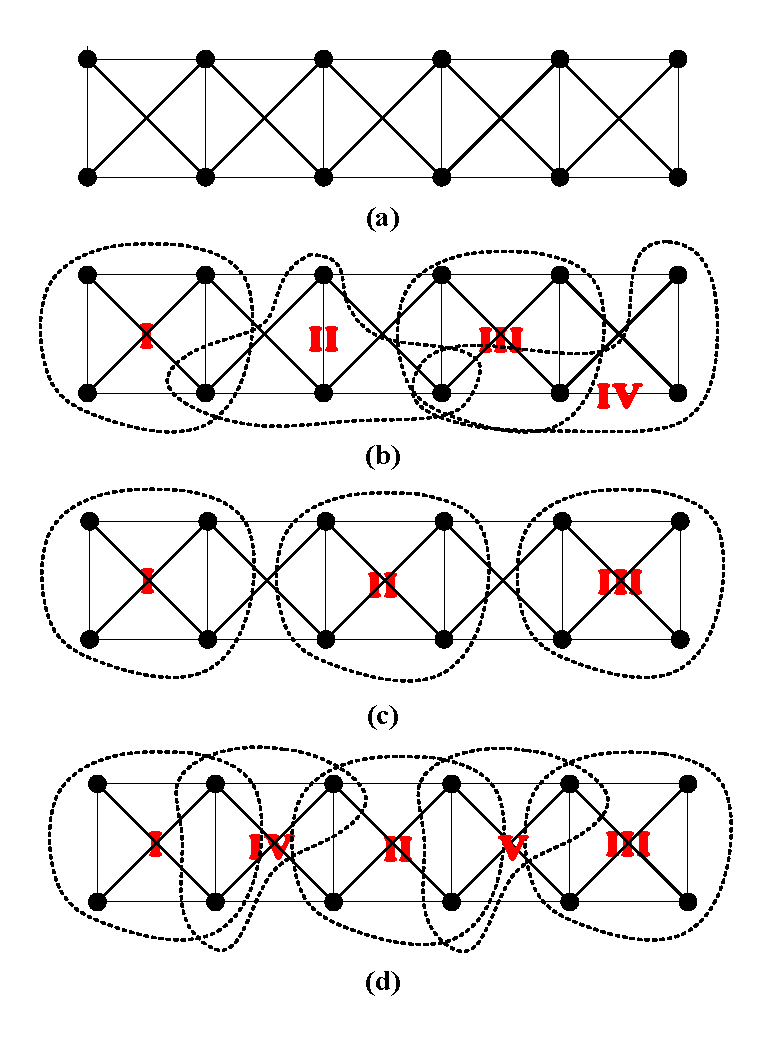
\includegraphics[width=.3\textwidth,height=.35\textwidth]{AlgorithmExampleNew.eps}
	\caption{Example of using the Proposed Algorithms (a) Graph G(V,E), (b) The 4 Clusters Generated from the \(1^{st}\) Algorithm (c) Isolated Cluster Groups from the \(2^{nd}\) Algorithm (e) Final 5 Clusters from the \(2^{nd}\) Algorithm}
	\label{fig:AlgorithmExampleNew}
\end{figure}
\end{comment}


\subsection{Distributed Algorithm}
Based on our first centralized algorithm, we propose a distributed solution. In this solution, each node only needs its one-hop neighbors information and communicates only with its one-hop neighbors. The clustering will start at a single controller node which usually is the sink node of the network.

Similar to Algorithm \ref{algo:greedy1}, each newly created cluster will be connected to at least one of the existing clusters. In the distributed algorithm, each node will maintain two lists of neighbors: unclustered and clustered. The lists will be sorted according to each neighbor's own number of unclustered neighbors. The nodes with fewer unclustered neighbors will do clustering or join other clusters first. This is done by assigning each node's execution of the algorithm to a specific time slot.

Each node has only three roles during clustering: unclustered, CM (cluster member) and CH. We illustrate the pseudo code based on the three roles in Algorithm \ref{algo:selectionsender}.

\begin{algorithm}
\begin{algorithmic}[1]
\REQUIRE \(n_{opt}\), \(p\), unclustered neighbors \(un\), clustered neighbors \(cn\) (\(un\) and \(cn\) are both sorted in increasing order according to the number of unclustered neighbors)
\IF {self is unclustered}
	\STATE Self becomes CH
\ENDIF
\IF {self is CH}
	\STATE Select one node from \(cn\) as its member
	\IF {\(size(un)\geq n_{opt}\)}
		\STATE Construct the cluster as size of \(n_{opt}\) by selecting first \(n_{opt}\) nodes from \(un\) as CM
	\ELSIF{\(n_{opt}>size(un)\geq p\)}
		\STATE Construct a cluster by selecting all nodes in \(un\) as CM
	\ELSE
		\STATE First construct a cluster by selecting all nodes in \(un\) as CM then select more nodes from \(cn\) as CM until \(cluster\_ size=p\)
	\ENDIF
\ELSIF {self is CM}
	\STATE Broadcast a message to all neighbors saying the status is currently CM.
\ENDIF
\STATE \(an=merge(un, cn)\)
\FORALL {\(n\in an\) that haven't been assigned a time slot}
	\STATE Assign time slot \(t[i]\) to \(n\) where \(i\) is the index of \(n\) in \(an\)
\ENDFOR
\end{algorithmic}
\caption{Distributed algorithm for clustering}
\label{algo:selectionsender}
\end{algorithm}

Each node will not execute the algorithm until the start of its own time slot. The input \(p\) is the minimum cluster size constraint and \(n_{opt}\) is the calculated optimal cluster size. Once a CH decides to choose certain node as CM, it will send a message \(req_{ch}\) and the corresponding CM will send \(acpt_{ch}\) to acknowledge the selection. After the execution of the algorithm on a node, an unclustered node will become CH. At the end of the algorithm, each node will merge all its neighbors into one sorted list and assign time slots. The duration of the time slot is large enough so that a CH can perform the selection. \(t[i]\) is the \(i^{th}\) time slot from the end of the current time slot. It can be easily seen that the generated clusters from the distributed algorithm can satisfy all the constraints.

Informally, it can be easily shown that the distributed algorithm is correct as the solution it produces will satisfy all the constraints:
\begin{itemize}
\item Since all nodes will be given a time slot to run the algorithm, the clusters will eventually cover the whole network.
\item The clustering starts at the controller node and all the later CHs will first select a CM from its \(cn\). Therefore, all the clusters will be connected.
\item CH only selects CM within its one-hop neighbors, and the CHs will not remove its role as CH so all clusters will be one-hop.
\item For each CH, it will ensure the cluster size is at least \(p\) by selecting additional CM until the cluster size reaches either \(p\) or \(n_{opt}\).
\end{itemize}
\cleardoublepage

\floatname{algorithm}{Procedure}
\chapter{System Implementation}
\label{chapter:implementation}
Since the goal of using middleware is to support application development. In this chapter we illustrate, how PSWare can be implemented for different applications.

\section{ITS Implementation Using PSWare}
We use our middleware to implement a traffic management prototype system in our testbed. The application architecture is shown in Figure \ref{fig:appdemo}. PSWare acts as the interface between WSN and application. On the application side, we have a web server where application-specific event templates are defined there. In the traffic management, we have defined events such as traffic jam and collision. Then the application users can subscribe the service by making use of the event templates. They can further refine their application requirements by providing parameters to the event templates.

\begin{figure}
\centering
\figurecurrentwidth{demo}
\caption{Demo application architecture}
\label{fig:appdemo}
\end{figure}

\subsection{Pre-defined Events}
In order for the users to use our middleware easier, we have provided some pre-defined event templates. With adjustable parameters. Listing \ref{lst:carevent} shows the most basic event - a car event in the system. All the attributes of the event can be directly obtained from the sensor nodes. The user can further add their own defined filters such as selecting only cars from certain road or selecting a car with pre-defined ID.

\begin{lstlisting}[caption=Car event, label=lst:carevent]
Event CarEvent {
	int roadID=System.roadID;
	int carID=System.carID;
	int posID=System.posID;
	int speed=System.speed;
}
\end{lstlisting}

Based on the basic car event, we can further make use of it and define a traffic jam event as shown in Listing \ref{lst:trafficjam}. In the example, we defined a traffic jam as having more 3 cars on a single road section.

\begin{lstlisting}[caption=Traffic jam event, label=lst:trafficjam]
Event TrafficJam {
	int roadID=System.roadID;
	int carNo=count(c);
} on {
	CarEvent c;
} where {
	roadID=1 &&
	carNo>3
}
\end{lstlisting}

Another type of event is car collision event. It is defined in terms of two car events. Listing \ref{lst:carcollision} defines a collision event on a road if the two car's speed are above certain threshold and their distance are too close.
\begin{lstlisting}[caption=Car collision event, label=lst:carcollision]
Event Collision {
	int roadID1=c1.roadID;
} on {
	CarEvent c1, c2;
} where {
	c1.roadID==c2.roadID &&
	c1.speed-c2.speed>5 && 
	c1.posID-c2.posID<2 
}
\end{lstlisting}

\subsection{User Interface Design}
We use a graphical user interface (GUI) to visualize the relations between events. Users can also specify their parameters on the given event templates. For example, for a traffic jam event in Figure \ref{fig:guitrafficjam}, user can further specify the condition for a traffic jam such as the number of cars waiting on a road. Similarly, for collision events \ref{fig:guicollision}, the user can specify the condition for such kind of events. Moreover, the user can also choose to monitor certain cars in the system for the collision event. This can be done by adding a parameter in the car events.

\begin{figure}
\centering
\subfloat[Traffic jam GUI]{\label{fig:guitrafficjam}\figurehalfwidth{guitrafficjam}}
\subfloat[Collision GUI]{\label{fig:guicollision}\figurehalfwidth{guicollision}}
\caption{GUI Design}
\label{fig:gui}
\end{figure}

\subsection{Customized Event Detection for ITS}
Intelligent transportation system may cover many application areas including collision avoidance, traffic light control and vehicle tracking. All these applications require the detection of vehicles. In this paper, we consider the scenario where sensor nodes are deployed as road side units (RSU) \cite{klein:its}. To detect vehicles in such a model, the sensors should be waken up as the vehicles are driving along the roads. The procedure for nodes' wake-up and forwarding is shown in Procedure \ref{algo:itsForward}. We use the following notations in the procedure:
\begin{itemize}
\item \(V=\{v_1, v_2 \cdots \}\): the sensor nodes that come next on the road. For the sensors on the road, \(\|V\|=1\) but for the sensors next to the crossroads, \(\|V\|>1\)
\item Vehicle events \(e_i\) which are either detected locally or received from another node.
\end{itemize}

\begin{algorithm}
\begin{algorithmic}[1]
	\IF {detected vehicle event \(e_i\)}
		\FORALL {\(v_n\in V\)}
			\STATE forward \(e_i\) to \(v_n\)
		\ENDFOR
	\ENDIF
	\IF {received vehicle event \(e_i\) from \(v_m\)}
		\STATE start data collection
		\IF {detected vehicle event \(e_j\)}
			\STATE select \(e_i\) and \(e_j\) for composite event detection
		\ELSE
			\STATE wait for event to expire
		\ENDIF
		\STATE stop data collection
	\ENDIF
\end{algorithmic}
\caption{Event forwarding for ITS}
\label{algo:itsForward}
\end{algorithm}

Except for the sentry node, nodes will not actively collect data until they receive messages from others. Once the event from the previous node on the road is received, it will be selected for composite event detection.
\section{SHM Implementation Using PSWare}
Apart from the ITS applications, we also implement an SHM prototype system. As discussed in the previous chapter, our SHM system involves the following steps:
\begin{enumerate}
\item Establish clusters in the network
\item Data sampling and processing to obtain the mode shape
\item Detect possible damage based on the mode shape
\end{enumerate}

\begin{figure}
\centering
\figurecurrentwidth{shm-flow}
\caption{SHM Operation Flow}
\label{fig:shm-flow}
\end{figure}

When developed using PSWare, the operation flow is shown in Figure \ref{fig:shm-flow}. First, the event subscription will trigger the network to cluster. Then data will be sampled. During data sampling, we store the sampled data in an internal buffer. Domain experts use modal analysis to obtain the mode shape. Modal analysis is implemented as a special instruction by the domain experts. Once the results are obtained, they will be published to the subscribers.

Since the modal analysis part requires a lot of domain knowledge and is not the focus of this work, in this section, we primarily discuss how the clustering algorithm can be integrated in PSWare. For our prototype system, we have one sink node and the subscriptions are disseminated through the sink node. Such setup is similar to many existing SHM system where the data are transmitted to a monitoring station for damage detection.

\subsection{Neighbor Information Exchange}
The sensor nodes exchange information periodically. Each sensor node maintains the following information:
\begin{itemize}
\item Its own clustering status. There are three possible values: UC (unclustered), CH (cluster head) and CM (cluster member)
\item Its neighbor table with clustering status: \(table_n\)
\end{itemize}

Each node \(v_n\) periodically broadcasts messages \(msg_n\) which is its \(table_n\). The procedure is shown in Procedure \ref{algo:table_n}.

\begin{algorithm}
\begin{algorithmic}[1]
\REQUIRE \(v_n\rightarrow msg_n\)
	\FOR {each entry \(t'\) in \(msg_n\)}
		\IF {\NOT exists \(t'\rightarrow fid_n\) in \(table_n\)}
			\STATE \(addTo(table_n, t')\)
		\ENDIF
		\FOR {each entry \(t\) in \(table_n\)}
			\IF {\(t\rightarrow status != t'\rightarrow status\)}
				\STATE \(t\rightarrow status != t'\rightarrow status\)
			\ENDIF
		\ENDFOR
	\ENDFOR
	\STATE \(msg_n \gets table_r\)
	\STATE \(periodically\_broadcast(msg_n)\)
\end{algorithmic}
\caption{\(table_n\) update}
\label{algo:table_n}
\end{algorithm}

\subsection{Clustering}
The actual clustering takes place after the subscription is received by individual sensor node. Internally, this is done by implementing the 'OPinstall' instruction. This is a special instruction which will be invoked when a sensor node receives new subscriptions. Please refer to Appendix for more information on the instructions.

\begin{algorithm}
\begin{algorithmic}[1]
\REQUIRE OPinstall
	\IF {self is sink}
		\STATE self.status = CH
	\ELSE
		\STATE self.status = UC
	\ENDIF
	\WHILE {self.status == UC}
		\STATE \(broadcast(msg_n)\)
		\STATE \(cost_n = MAX\)
		\FOR {each entry \(t\) in \(table_n\)}
			\STATE \(cost_n' = 0\)
			\FOR {each entry \(t'\) in \(t.table_n\)}
				\IF {\(t'.status == UC\)}
					\STATE \(cost_n' = cost_n' + 1\)
				\ENDIF
			\ENDFOR
			\STATE \(cost_n = min(cost_n', cost_n)\)
		\ENDFOR
		\STATE run\_uc();
	\ENDWHILE
	\IF {self.status == CM}
		\STATE run\_cm();
	\ELSE
		\STATE run\_ch();
	\ENDIF
\end{algorithmic}\caption{Clustering in SHM}
\label{algo:clustering-cost-calc}
\end{algorithm}

The procedure is shown in Procedure \ref{algo:clustering-cost-calc}. The procedure starts off from the sink node selecting itself to be a cluster head. The rest of the nodes are at first unclustered. Then each node will sort its neighbor's list according to the number of unclustered node that each neighbor has. This is to determine the neighbors which are more 'isolated' - those with most of its neighbors already clustered. The rest of the part has already been described in the previous chapter. Each node runs run\_uc(), run\_cm() and run\_ch() based on their clustering status. These functions implement the distributed time-slot based clustering algorithm discussed in the previous chapter.
\cleardoublepage

\chapter{System Evaluation}
\label{chapter:evaluation}
In this chapter, we analyze the performance of PSWare through analysis, simulation and experiments.

\section{Analysis on TED}
\label{sec:ceduanalysis}
Since TED is the essential algorithm used in our application, our analysis mainly focuses on its energy efficiency and delay. As discussed in our problem formulation, we message cost for measuring the energy efficiency in TED.

\subsection{Analysis on Message Cost}
In order to analyze the efficiency of TED without losing generality, we assume that sensor nodes are randomly deployed in a circular area with radius \(R\). We use distance to approximately measure the number of hops in order to calculate the message cost for event detection. There is no existing work that utilizes event types to detect composite events and it is also very hard to aggregate events without knowing their actual relations. Therefore, as a reference to compare the message cost, we use shortest path tree (SPT) algorithm where events are collected at the sink because their definitions are not considered for event detection.


We use a similar event model that has been introduced in Section \ref{sec:centralized} for analysis. Moreover, since the actual cost of TED will depend on event probabilities. We include such information in our model as well. Suppose we have two event types \(e_1\) and \(e_2\) which are the two sub-event types for a composite event \(e_3\) (i.e. \(e_1re_2=e_3, r\in R\)). The probability for \(e_1\) and \(e_2\) to occur is \(P(e_1)=p_1\) and \(P(e_2)=p_2\) respectively. The probability for \(e_3\) to occur when both \(e_1\) and \(e_2\) have occurred is \(P(e_3|e_1, e_2)=p_3\).

In TED, each node periodically broadcasts its routes to the fusion tables so that others can know how to reach the fusion points. Such cost is similar to many existing routing protocols in WSN such as \cite{rssiroute} where each node periodically broadcasts its route metrics to the sink for the purpose of link quality evaluation. Therefore, in TED, we mainly consider three types of messages which will be used:
\begin{itemize}
\item The overhead for initial event forwarding: \(cost_f\)
\item The overhead for the fusion points to send feedback: \(cost_b\)
\item The message cost for detecting the actual composite events: \(cost_d\)
\end{itemize}

Let the average distance between two random nodes in the square region be \(D\) and the average distance between a node and sink be \(d\). 
\begin{comment}
Then:
\begin{equation*}
D=\frac{2+\sqrt{2}+5\times ln(1+\sqrt{}2)}{15}\times|N|
\end{equation*}
Let the average distance between the event source and the event fusion points be \(d\).
\end{comment}

The cost for initial event forwarding will be: \(cost_f=2\times D\). In order to avoid the extra cost for building up the overlay for each fusion point to communicate with individual sensor nodes, the fusion nodes simply flood the feedback in the network. Therefore, the cost for the fusion points to send feedback will be: \(cost_b=D\times(|N|-2)\). The cost for detecting each individual event is: \(cost_d=D\). The total expected message cost using TED over a time period \(T\) is:
\begin{align*}
&cost_{TED}\\
=&cost_f+cost_b+T(p_1cost_d+p_2cost_d+p_3p_2p_1d)\\
=&D|N|+TD(p_1+p_2)+Tdp_1p_2p_3
\end{align*}

Here \(T\) is the \(expire_n\) used in \(table_e\). The total expected message cost using SPT over a time period \(T\) is:
\begin{equation*}
cost_{SPT}=d\times T(p_1+p_2)
\end{equation*}

To see when TED will cost less than SPT, we have:
\begin{align*}
cost_{TED}&<cost_{SPT}\\
D|N|+TD(p_1+p_2)+Tdp_1p_2p_3&<dT(p_1+p_2)\\
T((p_1+p_2)(d-D)-dp_1p_2p_3))&>|N|
\end{align*}

The inequality can be viewed as a trade-off between message cost saved by TED and the overhead. Simply speaking, TED can reduce message cost when:
\begin{itemize}
\item Fusion points are closer to event source
\item The probability of primitive event is high while the probability of the composite event is lower.
\item Each time after the \(table_e\) is constructed, it used for a relatively long period of \(T\) 
\end{itemize}

\subsection{Analysis on Delay}
In Algorithm \ref{algo:fusionPoint}, if there is no local match, the fusion point will wait for some time to see if there is any other events forwarded from other nodes. In this section, we study the delay of TED.
\begin{theorem}
\label{thm:delay}
Suppose the sensor nodes are randomly deployed in a circular area where sink is located at the center of the network, the events have a time span of \(t\), fusion points are randomly distributed with an average distance to other nodes of \(d\) and the sensor nodes forward the events at the speed of \(v\). Compared with SPT in the worst case, TED will introduce a delay of:
\begin{equation*}
delay_{TED}-delay_{SPT}=\frac{d}{v}+t
\end{equation*}
\end{theorem}

\begin{proof}
Let \(K\) be the average distance from an event to the sink. The delay of SPT will be \(delay_{SPT}=\frac{K}{v}\). To calculate the delay of the worst case in TED, we first need to calculate when TED will eventually forward the event to the sink. According to Algorithm \ref{algo:fusionPoint}, an event fusion point will forward the event if the sink is closer than any other fusion points. Suppose after \(k\) fusion points, the event will be forwarded to the sink. Then, we can get the following.
\begin{align*}
kd&\geq K\\
k&\geq \frac{2}{R}\frac{2}{\pi}\int_0^{\pi}2cos(\frac{\theta}{2})sin(\theta)[\theta-sin(\theta)]d\theta\\
k&\geq \frac{128R}{45\pi}\times\frac{2}{R}\\
k&\geq 1.81
\end{align*}

Therefore, we have:
\begin{align*}
delay_{TED}&=(\frac{d}{v}+t)(k-1)+\frac{D}{v}\\
delay_{TED}-delay_{SPT}&=(\frac{d}{v}+t)(k-1)\\
&=\frac{d}{v}+t
\end{align*}
\end{proof}
\begin{figure}
\centering
\subfloat[Possible fusion points]{\label{fig:fplvl3}\figurehalfwidth {fplvl3}}
\subfloat[Communication range]{\label{fig:communicationrange}\figurehalfwidth{communicationrange}}
\caption{Simulation environment}
\label{fig:simsetup}
\end{figure}

We have conducted both simulation and experiments on PSWare to evaluate its performance. The simulation is used mainly to validate our analytical results on TED while the experiments are done according to some real WSN-based applications in order to demonstrate the effectiveness and efficiency of PSWare.

\section{Simulation}
\label{sec:simulation}
We use simulation to validate our analytical results. Our simulation is based on TOSSIM \cite{tossim}. We have \(127\times 127\) sensor nodes placed on a square space. We use both even distribution and random distribution of the fusion points. Similar to our analysis, we divide the whole area into small squares and deploy equal number of fusion points for each square. Each sensor node is able to communicate with its nearby neighbors. To simulate the event detection, we first randomly generate event sources in the network. Then based on these event sources, we further generate more sub-events that have relations and let the sensor node detect the composite events. We study the performance of TED under different parameters such as event distribution, event probability, and deployment approach. In the figures, TED-R represents distributed TED with random fusion point deployment and TED-E represents distributed TED with even fusion point deployment.

\begin{figure}
\centering
\figurecurrentwidth{size-distance30}
\caption{Average event distance: 30}
\label{fig:sim-size-distance30}
\end{figure}

Similar to our analysis, we use SPT as a reference to compare with TED so as to see how much cost we can save if we detect the events using their relations. For simplicity, we assume in SPT approach, the events can always be aggregated at the shared paths. We study the performance of TED under different parameters such as fusion point deployment, event distance, event size and event probability.

To obtain more accurate results, we repeat the simulation for 10,000 times for each of the graph we discuss in the following sections. For each set of data, the standard deviation is less than 0.5.

\subsection{Impact of Event Distance}
The first parameter we study is the distance between events. More precisely, we study the average event distance where it is defined as the average of all the distance between any two events in the network. Figure \ref{fig:sim-size-distance30} shows the result when average event distance equals to 30. As we can see, SPT costs the most energy. Among the different versions of TED, TED-C costs slightly higher energy while TED-E costs the lowest amount of energy.

\begin{figure}
\centering
\figurecurrentwidth{size-distance40}
\caption{Average event distance: 40}
\label{fig:sim-size-distance40}
\end{figure}

The next set of simulation results are shown in Figure \ref{fig:sim-size-distance40}. In this figure, we can see as the event distance becomes greater, the average energy cost has also increased accordingly. This is inevitable because the nodes will have relay the events for more number of hops in order to detect the composite events. Note that our X-axis represents event size. We will get into more details about the impact of event size in the next section.

\begin{figure}
\centering
\figurecurrentwidth{size-distance50}
\caption{Average event distance: 50}
\label{fig:sim-size-distance50}
\end{figure}

The last set of results for event distance is shown in Figure \ref{fig:sim-size-distance50}. In this figure, the event distance is set to be 50. Note that this is already half of the network dimension. Such scenario should cover a lot of WSN applications where the events need to be transmitted for a long distance to be further processed. As we can see from the figure, when the event distance becomes larger, the results have also become more stable. This is because as the distance becomes larger, relay cost has become the dominant cost for the event detection.

In summary, as we can see from all the figures, TED can save some energy in comparison with SPT. However, among all the simulation parameters as we will see in the following sections, event distance does not seem to be a critical factor where TED can save a lot of energy.

\subsection{Impact of Event Size}
\begin{figure}
\centering
\figurecurrentwidth{distance-size5}
\caption{Average event size: 5 nodes}
\label{fig:sim-distance-size5}
\end{figure}

The next factor we are going to study is event size. This factor is interesting to our simulation because different event size may have different effect on the number of nodes that are needed to detect more than one events. It can, therefore, affect the choice of event fusion points since sometimes it may be better to choose the nodes that can detect multiple events as the fusion points.

The first set of results are displayed in Figure \ref{fig:sim-distance-size5}. Here we define the average event size to be the average number of nodes that will be involved to detect a specific primitive event. Furthermore, the nodes must be connected by themselves. If, for example, an event spans nodes that are not connected by themselves, then we can split such events into multiple sub-events where all the nodes involved in detecting each sub-event are connected by themselves.

\begin{figure}
\centering
\figurecurrentwidth{distance-size10}
\caption{Average event size: 10 nodes}
\label{fig:sim-distance-size10}
\end{figure}

The next set of results are shown in Figure \ref{fig:sim-distance-size10}. Since based on our previous results, event distance is not a major factor for TED to save energy, we use it as the X-axis in our simulation for reference. Since the event size has increased from 5 to 10 nodes, we also need to decide which nodes out of all the event detection nodes will be used as the decision maker for the event. In order to have a reasonably easy function to calculate the cost without losing generality, we choose the node at the geographical center of the primitive event to be the detector node.

As we can see, SPT still incurs the highest cost. Among all the TED variations, the centralized version has relatively higher cost while the distributed TED with even fusion point deployment has the lowest cost. This is because the centralized version will introduce control overhead and the even fusion point deployment strategy guarantees that each event can find a fusion point within certain number of hops.

\begin{figure}
\centering
\figurecurrentwidth{distance-size15}
\caption{Average event size: 15 nodes}
\label{fig:sim-distance-size15}
\end{figure}

Our last set of results are shown in Figure \ref{fig:sim-distance-size15}. In this set of results, we set the average event size to be 15 nodes. Note that this is already a quite large event size since on average, it spans 15 nodes. It may be suitable for many applications where the aggregate functions such as average or sum need to be evaluated. The results are similar to the previous ones in the sense that SPT has the highest energy cost while TED-E has the lowest. However, this set of results are more stable and consistent than the previous set. This is because as the event size becomes larger, it is easier to cover more number of nodes and therefore having more overlapped ones. TED may make use of such overlapped nodes to select fusion points. Therefore, TED will have a wider choice as the event size becomes larger and the results will become more stable.

In summary, according to all the results shown in this section, we can draw conclusion that event size is not a major factor that will decide the amount of energy that TED could save. While TED does perform better than SPT in respect of event size and event distance, we still need to study more factor to see if it can perform even better.

\subsection{Impact of Event Probability}

\begin{figure}
\centering
\figurecurrentwidth{prob-size5-dist10}
\caption{Event size: 5, distance: 10}
\label{fig:sim-prob-size5-dist10}
\end{figure}

Since we have studied two parameters in our previous sections, we will study the last factor in accordance to the previous factors we have studied and see how it can affect the performance of TED. Figure \ref{fig:sim-prob-size5-dist10} shows our first set of results. Our first set of results look promising since all variations of TED saves significant amount of energy than SPT.

\begin{figure}
\centering
\figurecurrentwidth{prob-size5-dist20}
\caption{Event size: 5, distance: 20}
\label{fig:sim-prob-size5-dist20}
\end{figure}

Our second set of results are shown in Figure \ref{fig:sim-prob-size5-dist20}. Since we have already concluded in our previous section that event size is not a major factor that will affect the performance of TED, in this set of results, we fix the event size while increasing the event distance for each set. Then within each set, we use the event probability as the X-axis to have a more direct view of the relation between event probability and energy cost.

As shown in the figure, SPT still has the highest energy cost. For TED, the energy cost is particular low while the event probability is less than 50\%. This is because with TED, we can effectively filter the primitive events if they are not going to lead to higher level of composite events.

\begin{figure}
\centering
\figurecurrentwidth{prob-size5-dist30}
\caption{Event size: 5, distance: 30}
\label{fig:sim-prob-size5-dist30}
\end{figure}

Our third set of results are shown in Figure \ref{fig:sim-prob-size5-dist30}. This set of results are consistent with the previous two sets. For SPT, the energy cost does not change much with the event probability. For all versions of TED, the event detection cost is below 40 when the event probability is 20\%. This is because with such a low probability, many of the primitive events have been filtered before they get a chance to be fused for higher level composite event detection.

Among the three variations of TED, we can see TED-C has slightly higher cost than the other two. This is because of the overhead introduced in the centralized approach where the event fusion points need to be selected by the sink node. For the distributed variations, TED-R and TED-E have similar performance. TED-E has slightly lower energy cost because of its even distribution. Each sensor nodes may find a fusion point in a bounded distance.

\begin{figure}
\centering
\figurecurrentwidth{prob-dist20-size5}
\caption{Event distance: 20, size: 5}
\label{fig:sim-prob-dist20-size5}
\end{figure}

In our previous results. We studied the impact event probability by fixing event size while increasing the event distance. The fixed event size was set to be 5 which is small enough to be considered as atomic event size. As we have also studied the impact of event size in our previous sections, for the sake of completeness, we also perform another three set of simulations to study the event probability while fixing the event distance.

Since our network size is 127 by 127, we choose the fixed average event distance to be 20. This is around \(\frac{1}{6}\) of the network dimension which is probably representative enough for many WSN-based application. Our fourth set of results are presented in \ref{fig:sim-prob-dist20-size5}. In the figure, we can also see TED can save significant amount of energy in comparison with SPT.

\begin{figure}
\centering
\figurecurrentwidth{prob-dist20-size10}
\caption{Event distance: 20, size: 10}
\label{fig:sim-prob-dist20-size10}
\end{figure}

Our fifth set of results is shown in Figure \ref{fig:sim-prob-dist20-size10}. On the X-axis, the event probability spans from 20\% to 60\%. Note that for composite events, this is a conditional probability when all the sub-events happen. For instance, if a composite event \(e_3\) comes from two sub-events \(e_1\) and \(e_2\). Then we have the following:
\begin{align*}
P(e_3) = P(e_1) \times P(e_2) \times P(e_3|e_1, e_2)
\end{align*}

\begin{figure}
\centering
\figurecurrentwidth{prob-dist20-size15}
\caption{Event distance: 20, size: 15}
\label{fig:sim-prob-dist20-size15}
\end{figure}

Our final set of results is shown in Figure \ref{fig:sim-prob-dist20-size15}. Similar to our previous sets of results, TED can save around 50\% - 60\% of energy cost compared with SPT.

In summary, we can find our simulation results agree with our analytical results. The energy cost of TED is linearly proportional to the event probability while the energy cost of SPT has little difference in regard to probability changes. This characteristic will make TED especially effective for applications where the primitive events happen very frequently while the composite events happen rarely.
\section{Experiments}
\label{sec:experiments}
As described in Section \ref{sec:ceduanalysis}, the performance of TED heavily depends on the actual WSN applications because different applications may have different very different event definitions. In this section, we study some of thes WSN applications and find out how well TED performs.

We have implemented TED on MicaZ based on the existing middleware layer as in \cite{lai:psware}. Similar to Section \ref{sec:ceduanalysis}, we implemented a module that does opportunistic data aggregation based on the existing routing protocol provided by TinyOS for comparison.

We compare the performance using the following metrics:
\begin{itemize}
\item Message cost: this is obtained by setting up a counter inside the sensor node. The counter will be written into flash after the experiment so that we can retrieve it.
\item Event detection delay: we measure the time between the subscription is disseminated and the event is notified.
\end{itemize}

\begin{figure}
\centering
\subfloat[The sensor node]{\label{fig:carParkSensor1}\figurehalfwidth{carParkSensor1.JPG}}
\subfloat[The light sensor]{\label{fig:carParkSensor2}\figurehalfwidth{carParkSensor2.JPG}}
\caption{Car park sensor platform}
\label{fig:carParkSensor}
\end{figure}

\subsection{Application Case One: Car Park}
Our first application case is an intelligent car park \cite{tang:carpark}. We deployed some micaz sensor nodes for the application. For simplicity, we use light sensor to detect the presence of a vehicle. For better communication, the sensor nodes are attached close to the ceiling instead of on the ground. The light sensor on each node is connected through an extended cable as shown in Figure \ref{fig:carParkSensor}. 

\begin{figure}
\centering
\figurecurrentwidth{carParkDeployment}
\caption{Car park sensor deployment}
\label{fig:carParkDeployment}
\end{figure}

The deployment of the sensor nodes is shown in Figure \ref{fig:carParkDeployment}. In such a system, the management is interested in the number of park spaces and the location of them \cite{tang:carpark}. The primitive events for such a system will be the availability of individual car park spaces. Based on the primitive event, if we want to get notified when the parking spaces near the exit become available, then we just need to define composite events which locate the spaces with certain IDs. Th event definitions are shown in Listing \ref{lst:carPark}. Here, the composite event takes two primitive events for parking space \(1\) and \(2\) which are close to the exit. The experimental results are shown in Figure \ref{fig:carParkResults}. In this application, we primarily consider only the message costs because the delay isn't that important in such a system. The message cost is highest during rush hour when there are a lot of cars entering and leaving the car park. The message cost saved by TED is around 10-20\% regardless of the total messages.

\begin{lstlisting}[caption=Event definition for a car park, label=lst:carPark]
Event ParkSpaceEvent {
	int id=System.id;
	int time=System.time;
	int light=System.light;
} where {
	light>THRESHOLD
}
Event CarParkEvent {
	int id=System.id;
} on {
	ParkSpaceEvent e1, e2;
} where {
	e1.id==1 ||
	e2.id==2 ||
	e1.time-e2.time<10
}
\end{lstlisting}

\begin{figure}
\centering
\subfloat[With three fusion points]{\label{fig:carParkResult1}\figurehalfwidth{carParkResult1}}
\subfloat[With four fusion points]{\label{fig:carParkResult2}\figurehalfwidth{carParkResult2}}
\caption{Car park experiment results}
\label{fig:carParkResults}
\end{figure}

\subsection{Application Case Two: Transportation Systems}
Apart from intelligent car park, another related application is WSN-based intelligent transportation system \cite{lai:its}. We also use the Micaz nodes to deploy such an application using our TED. Before we do the field test, we first perform some simple test on our lab testbed, iTranSNet. Figure \ref{fig:itransnet} shows our testbed setup. In such testbed, we use some model cars to run a platform so that the sensor nodes can detect them.

\begin{figure}
\centering
\subfloat[Our iTranSNet testbed]{\label{fig:testbed-road}\figurehalfwidth{testbed-road.JPG}}
\subfloat[The model cars for iTranSNet testbed]{\label{fig:testbed-car}\figurehalfwidth{testbed-car.JPG}}
\caption{Lab testbed for transportation systems}
\label{fig:itransnet}
\end{figure}

In order to test different scenarios, we defined different event types for potentially different ITS applications. Listing \ref{lst:basicCar} shows one of the most basic events for detecting a single vehicle. 
\begin{lstlisting}[caption=Event definition for detecting a single vehicle, label=lst:basicCar]
Event CarEvent {
	int time=System.time;
	int magnetic=System.magnetic;
	int location=System.location;
} where {
	magnetic>THRESHOLD
}
\end{lstlisting}

\begin{figure}
\centering
\subfloat[Message cost]{\label{fig:itransnet1}\figurehalfwidth{itransnet1}}
\subfloat[Delay]{\label{fig:itransnet2}\figurehalfwidth{itransnet2}}
\caption{Experimental results on lab testbed: iTranSNet}
\label{fig:itransnetResults}
\end{figure}

Listing \ref{lst:overspeeding} defines an event for detecting an over speeding vehicle.
\begin{lstlisting}[caption=Event definition for over speeding, label=lst:overspeeding]
Event SpeedEvent {
	int speed=(e1.location-e2.location)/(e1.time-e2.time);
} on {
	CarEvent e1, e2;
} where {
	e1.time>e2.time &&
	speed>THRESHOLD
}
\end{lstlisting}

Listing \ref{lst:trafficcount} defines an event for detecting a traffic jam.
\begin{lstlisting}[caption=Event definition for traffic jam, label=lst:trafficcount]
Event TrafficJam {
	int count=count(e1);
	int roadID=e1.roadID;
} on {
	CarEvent e1;
} where {
	roadID==CERTAIN_ROAD &&
	count>THRESHOLD
}
\end{lstlisting}

Different from the car park application, such applications are more delay sensitive. So we also measured the time delay for the event detection. We performed the testing on all the event types defined. The results are presented in Figure \ref{fig:itransnetResults}. The experimental results basically agree with the simulation results and show PSWare can save energy without too much delay.

After PSWare passes lab testing, we further deployed it in the real environment. The deployment in the real environment is shown in Figure \ref{fig:itsSensor}.

\begin{figure}
\centering
\subfloat[Road side sensor nodes]{\label{fig:itsSensor1}\figurehalfwidth{itsSensor1.JPG}}
\subfloat[Sensor nodes on the lamp]{\label{fig:itsSensor2}\figurehalfwidth{itsSensor2.JPG}}
\caption{Sensor nodes for transportation systems}
\label{fig:itsSensor}
\end{figure}

The event definitions are the same as those we have used for our indoor test. The results are shown in Figure \ref{fig:itsResults}. Similar to the car park application, TED can save 10-20\% energy while the delay is only a couple of milliseconds.
 
\begin{figure}
\centering
\subfloat[Message cost]{\label{fig:itsResult1}\figurehalfwidth{itsResult1}}
\subfloat[Delay]{\label{fig:itsResult2}\figurehalfwidth{itsResult2}}
\caption{Experimental results on the real roads}
\label{fig:itsResults}
\end{figure}

\subsection{Application Case Three: Indoor Monitoring}
Our final application is related to smart building. We consider the application scenario where the sensor nodes are deployed in a building so that the temperature can be monitored. Such an application can probably be useful for certain types of context aware pervasive applications. For example, the air conditioner can be adjusted if several adjacent rooms' temperature rises too fast. The primitive and composite event definitions are shown in Listing \ref{lst:indoorEvents}.

\begin{lstlisting}[caption=Event definition for indoor monitoring, label=lst:indoorEvents]
Event SingleTemp {
	int id=System.id;
	int temperature=System.temperature;
} where {
	temperature>THRESHOLD
}
Event CompositeTemp {
} on {
	SingleTemp e1, e2, e3;
} where {
	e1.id==1 &&
	e2.id==2 &&
	e3.id==4
}
\end{lstlisting}

The primitive event simply tests if the temperature passes certain threshold and the composite event is the conjunction of several primitive events. We deployed the some Micaz nodes in different rooms in our building as shown in Figure \ref{fig:indoorDeployment}.

\begin{figure}
\centering
\figurecurrentwidth{indoorDeployment}
\caption{Deployment of the senosr nodes for indoor monitoring}
\label{fig:indoorDeployment}
\end{figure}

The experimental results is shown in Figure \ref{fig:itsResults}. The results show that TED can save the message cost by 10-20\%.

\subsection{Application Case Four: SHM}
In our experiments, we consider the application for WSN-based Structural Health Monitoring (SHM) system. The objective of such system is to detect damages on structures such as buildings and bridges if they occur. Event detection is important in these applications because the SHM sensors will introduce high energy consumption during damage detection. It is therefore more desirable to wake them up only upon the occurrence of certain events \cite{jangshm}.

Figure \ref{fig:testbed} shows our WSN-SHM testbed. In our experiment, we defined a scenario where the sensor nodes will start to collect the data when a certain vibration pattern is detected. The vibration is detected if the one sensor on the top and another one on the bottom of the model read the vibration data that satisfy certain criteria. The event definition is shown in Listing \ref{lst:shm}.

\begin{figure}
\centering
\subfloat[With 2 fusion points]{\label{fig:indoorResult1}\figurehalfwidth{indoorResult1}}
\subfloat[With 3 fusion points]{\label{fig:indoorResult2}\figurehalfwidth{indoorResult2}}
\caption{Experiments for temperature monitoring}
\label{fig:indoorResult}
\end{figure}

\begin{lstlisting}[caption=Event definition for SHM, label=lst:shm]
Event Vibration {
	data=System.Vibration;
} where {
	data>THRESHOLD1
}
Event CompVibration {
} on {
	Vibration e1 and
	Vibration e2
} where {
	e1.location=='top' &&
	e2.location=='bottom' &&
	e1.data-e2.data>THRESHOLD2
}
\end{lstlisting}

\begin{figure}
\centering
\subfloat[The testbed]{\label{fig:testbed}\figurehalfwidth{CIMG3851.JPG}}
\subfloat[Parameters used in the experiments]{\label{fig:experimentModel}\figurehalfwidth{experimentModel}}
\caption{PSWare experiment setup}
\label{fig:experimentSetup}
\end{figure}

With the help of our testbed, we can manually generate events by hitting the model in our testbed. Similar to our simulation, we implemented a na\"{i}ve event detection method where the nodes simply use the existing routings provided by TinyOS \cite{nesc} and detect events opportunistically. We implement two modules for both our TED and the opportunistic filtering where only the primitive events are filtered. In order to create multi-hop communication, we adjust the nodes communication range so that they can only communicate with nearby neighbors. For TED, we use tested both the centralized and the distributed versions and for the distributed version. For TED, we have the parameters set as shown in Figure \ref{fig:experimentModel}.

Figure \ref{fig:exp-all} shows all our experimental results. In addition to energy efficiency, we also studied delay. We calculate the delay for TED as the duration between the time that na\"{i}ve approach detects the event and the time that TED detects them. This is because na\"{i}ve approach sends all the detected primitive events directly to the sink and the delay is only introduced by the multi-hop routing latency while both TED have additional delay in detecting the events. The experimental results are expected because TED slightly introduces more delay when doing the fusion points selection. The results on message cost is similar to our simulations.

\begin{figure}
\centering
\subfloat[Message cost]{\label{fig:exp-cost-probability}
\figurehalfwidth{exp-cost}}
\subfloat[Delay]{\label{fig:exp-delay-probability}
\figurehalfwidth{exp-delay}}
\caption{Experimental results for SHM}
\label{fig:exp-all}
\end{figure}

\cleardoublepage

\section{Conclusion}
\label{sec:conclusion}
In this paper, we presented PSWare, a flexible middleware framework for composite events processing. PSWare uses a flexible architecture where different event detection mechanisms may easily integrated. We described the design of PSWare and explained how it can be customized for different applications. Then we gave two examples of using PSWare. The first one implements a more general composite event algorithm while the second one uses an application-specific event detection approach. Based on our implementation, we performed experiments and demonstrate the effectiveness of PSWare for prototyping and performance comparison.
\cleardoublepage

\bibliographystyle{plain}
\renewcommand{\bibname}{References} % changes the header; default: Bibliography
\bibliography{../references/wsn-general,../references/wsn-aggregation,../references/wsn-middleware,../references/event-detection,../references/wsn-pubsub,../references/edl,../references/pubsub,../references/algorithms,../references/shm,../references/maths,../references/publist}

\appendix
\section{Complete List of the Instructions for EDF}
\label{appendix:isa}
In this section, we show the complete list of instructions currently used by our Event Detection Framework (EDF). We also briefly describe the function and the usage of each instruction.

\subsection{Basic Instructions}
The basic instruction deals with the most fundamental operations. Since the instruction uses a stack-based architecture in order to reduce the code size, most of the instructions that fall into this category deal with the operations related stacks.
\begin{itemize}
\item \emph{OPpush}: this instruction is used to push an operand to the top of the stack.
\item \emph{OPpop}: this instruction is used to pop and discard an operand from the top of the stack.
\item \emph{OPcopy}: duplicates the top operand of the stack
\item \emph{OPhalt}: once this instruction is reached, the VM will stop execution.
\end{itemize}

\subsection{Operators}
Basic mathematical operators:
\begin{itemize}
\item \emph{OPadd}: pops two operands off the top of the stack, add them together and push the result back to the top of the stack.
\item \emph{OPmult}: pops two operands off the top of the stack, multiply them together and push the result back to the top of the stack.
\item \emph{OPsub}: pops two operands off the top of the stack, subtract the first popped number by the second one and push the result back to the top of the stack.
\item \emph{OPdiv}: pops two operands off the top of the stack, divide the first popped number by the second one and push the result back to the top of the stack.
\item \emph{OPmod}: pops two operands off the top of the stack, divide the first popped number by the second one and push the remainder back to the top of the stack.
\item \emph{OPinv}: pops one operand (n) off the top of the stack, calculate its inverse (-n) and push the result back.
\end{itemize}

Logical operators:
\begin{itemize}
\item \emph{OPand}: pops two operands off the top of the stack, calculate the logical and of them and push the result back to the top of the stack.
\item \emph{OPor}: pops two operands off the top of the stack, calculate the logical or of them and push the result back to the top of the stack.
\item \emph{OPxor}: pops two operands off the top of the stack, calculate the exclusive or of them and push the result back to the top of the stack.
\item \emph{OPnot}: pops one operand off the top of the stack, calculate the logical not of it and push the result back to the top of the stack.
\end{itemize}

Relational operators:
\begin{itemize}
\item \emph{OPeq}: pops two operands off the top of the stack, if the two operands are equal, push 1 to stack. Otherwise, push 0 to stack.
\item \emph{OPneq}: pops two operands off the top of the stack, if the two operands are equal, push 0 to stack. Otherwise, push 1 to stack.
\item \emph{OPgt}: pops two operands off the top of the stack, if the first operand is greater than the second one, push 0 to stack. Otherwise, push 1 to stack.
\item \emph{OPgte}: pops two operands off the top of the stack, if the first operand is greater than or equal to the second one, push 0 to stack. Otherwise, push 1 to stack.
\item \emph{OPlt}: pops two operands off the top of the stack, if the first operand is less than the second one, push 0 to stack. Otherwise, push 1 to stack.
\item \emph{OPlte}: pops two operands off the top of the stack, if the first operand is less than or equal to the second one, push 0 to stack. Otherwise, push 1 to stack.
\end{itemize}

Bitwise operators:
\begin{itemize}
\item \emph{OPshiftl}: pops two operands off the top of the stack, left shift the first popped number by the second one and push the result back to the top of the stack.
\item \emph{OPshiftr}: pops two operands off the top of the stack, right shift the first popped number by the second one and push the result back to the top of the stack.
\item \emph{OPland}: pops two operands off the top of the stack, calculate the bitwise and of them and push the result back to the top of the stack.
\item \emph{OPlor}: pops two operands off the top of the stack, calculate the bitwise or of them and push the result back to the top of the stack.
\item \emph{OPxor}: pops two operands off the top of the stack, calculate the bitwise exclusive or of them and push the result back to the top of the stack.
\item \emph{OPlnot}: pops one operand off the top of the stack, calculate its complement and push the result back to the top of the stack.
\end{itemize}

\subsection{Event-related Instructions}
\begin{itemize}
\item \emph{OPref}: whenever an event \(e\) is being evaluated, this instruction is invoked to obtain an instance of such event.
\item \emph{OPoffset}: this instruction is involved right after the 'ref' instruction, in order to access individual attributes of the event instance.
\item \emph{OPset}: if the attributes of an event need to be changed, this instruction will be used.
\item \emph{OPget}: the 'get' instruction does the opposite of 'set' instruction. It will simply retrieve content of a specific attribute in an event.
\item \emph{OPcreate}: is used to create a new instance of an event.
\item \emph{OPeval}: is used to determine if an event happens or not.
\item \emph{OPgc}: used by the event matcher for garbage collection.
\end{itemize}

\end{document}